\documentclass[12pt]{memoir}

\usepackage[letterpaper,left=3.0cm,right=2.5cm,top=3.0cm,bottom=3.0cm]{geometry}

% Style packages
\usepackage[utf8]{inputenc}
\usepackage{graphicx}
\usepackage{lmodern}
\usepackage{xcolor}
\usepackage{xspace}
\usepackage{amsmath}
\usepackage{mathtools}
\usepackage{array}
\usepackage{hhline}
\usepackage{titling}
\usepackage{wasysym}

% Physics packages
\usepackage{braket}
\usepackage{simplewick}

\usepackage{hyperref}
\usepackage[square, comma, numbers, sort&compress]{natbib}

% For CG coefficients
\makeatletter
\renewcommand*\env@matrix[1][*\c@MaxMatrixCols c]{%
  \hskip -\arraycolsep
  \let\@ifnextchar\new@ifnextchar
  \array{#1}}
\makeatother

% For license
\usepackage[
    type={CC},
    modifier={by},
    version={4.0},
]{doclicense}

\setsecnumdepth{subsubsection}
\maxtocdepth{subsection}

% Parskip-style
% \setlength{\parindent}{0pt}
\nonzeroparskip


% TODO
\newcommand{\XXX}[1]{\textcolor{red}{#1}}

% Text shortcuts
\newcommand{\mscheme}{\texorpdfstring{$m$-scheme}{m-scheme}\xspace}
\newcommand{\abinitio}{\textit{ab initio}\xspace}

% Units
\newcommand{\mev}{\, \text{MeV}}
\newcommand{\invfm}{\, \text{fm}^{-1}}

% Second quant
\newcommand{\crea}[1]{\ensuremath{a_{#1}^{\dagger}}}
\newcommand{\annih}[1]{\ensuremath{a_{#1}}}
\newcommand{\qpcrea}[1]{\ensuremath{b_{#1}^{\dagger}}}
\newcommand{\qpannih}[1]{\ensuremath{b_{#1}}}

% Commutators
\newcommand{\comm}[2]{\ensuremath{[#1, #2]}}
\newcommand{\anticomm}[2]{\ensuremath{\{#1, #2\}}}

% A-body operators
\newcommand*{\zerobodyop}[1]{\ensuremath{{#1}^{(0)}}}
\newcommand*{\onebodyop}[1]{\ensuremath{{#1}^{(1)}}}
\newcommand*{\twobodyop}[1]{\ensuremath{{#1}^{(2)}}}
\newcommand*{\threebodyop}[1]{\ensuremath{{#1}^{(3)}}}
\newcommand*{\abodyop}[1]{\ensuremath{{#1}^{(A)}}}

% Normal ordering
\newcommand{\nogen}[1]{\ensuremath{\text{N}\left[#1\right]}}
\newcommand{\novac}[1]{\ensuremath{\text{N}_{0}\left[#1\right]}}
\newcommand{\noref}[1]{\ensuremath{\text{N}_{\Phi}\left[#1\right]}}

% Normal ordered operators
\newcommand*{\hnozero}{\zerobodyop{\bar{H}}}
\newcommand*{\hnoone}{\onebodyop{\bar{H}}}
\newcommand*{\hnotwo}{\twobodyop{\bar{H}}}
\newcommand*{\hnothree}{\threebodyop{\bar{H}}}


% Ref state
\newcommand{\refgnd}{\ensuremath{\ket{\Phi}}}
\newcommand{\refhp}[2]{\ensuremath{\ket{\Phi_{#1}^{#2}}}}

% IM_SRG generators
\newcommand*{\genone}{\eta^{(1)}}
\newcommand*{\gentwo}{\eta^{(2)}}
\newcommand*{\genthree}{\eta^{(3)}}

% m-scheme basis
\newcommand*{\emax}{e_{\text{max}}}


% Specify which words shouldn't be hyphenated
\hyphenation{IMSRG}

\title{Analysis of three-body effects in the \\ in-medium similarity renormalization group}

\author{Matthias Heinz}

\date{\today}

% \DoubleSpacing
\allowdisplaybreaks

\begin{document}

\frontmatter{}

% Title
% \maketitle
%*******************************************************
% titlepage
%*******************************************************
\newlength{\titleheight}
\setlength{\titleheight}{100pt}
\begin{titlingpage}

\parbox{\textwidth}{

\includegraphics[height=20mm]{thesis/doc/tud_logo.pdf}
\\[.3cm]
\raggedright
{\hfill Fachbereich Physik \\
Institut f\"{u}r Kernphysik
}
}
\begin{center}

\vfill

{
    \centering
    \begingroup
    \setlength{\baselineskip}{1.cm}
    {\fontsize{13}{12}%\selectfont
        {\LARGE\textit{{Analysis of three-body effects in the \\ in-medium similarity renormalization group}}}}\\ % \Large \LARGE
    \endgroup
}

\vfill

{

    \large{Master's thesis} \\
    \vspace{3mm}
    \large{by Matthias Heinz} \\
    \vspace{3mm}
    \large{Submitted: October 13, 2020} \\
}

\vfill

\newcommand{\smallsize}{5pt}
\newcommand{\bigsize}{25pt}

{
    \begin{tabular}{lll}
        \multicolumn{3}{l}{Examiners:}                 \\ \\
         &
        \multicolumn{2}{l}{Prof.~Achim Schwenk, Ph.D.} \\ \\
         &
        \multicolumn{2}{l}{Dr.~Alexander Tichai}
    \end{tabular}
    \vfill
}

\end{center}
\end{titlingpage}

\cleardoublepage\noindent Analysis of three-body effects in the in-medium similarity renormalization group \\ \\
Master's thesis by Matthias Heinz \\ \\
First examiner report: Prof.~Achim Schwenk, Ph.D. \\
Second examiner report: Dr.~Alexander Tichai\\ \\
Submitted on October 13, 2020 \\
\hrule
\noindent Analyse von Dreiteilcheneffekten in der in-medium \"{A}hnlichkeitsrenormierungsgruppe \\ \\
Masterthesis von Matthias Heinz \\ \\
1.~Gutachten: Prof.~Achim Schwenk, Ph.D. \\
2.~Gutachten: Dr.~Alexander Tichai\\ \\
Tag der Einreichung: 13.~Oktober, 2020 \\

\vfill
\doclicenseThis
\clearpage

\cleardoublepage\section*{Erkl\"arung zur Abschlussarbeit gem\"a\ss\ \S\ 22 Abs.\ 7 und \S\ 23 Abs.\ 7 APB TU Darmstadt}

Hiermit versichere ich, Matthias Heinz, die vorliegende Master-Thesis gem\"a\ss{} \S\ 22 Abs.\ 7 APB der TU Darmstadt ohne Hilfe Dritter und nur mit den angegebenen Quellen und Hilfsmitteln angefertigt zu haben. Alle Stellen, die Quellen entnommen wurden, sind als solche kenntlich gemacht worden. Diese Arbeit hat in gleicher oder \"ahnlicher Form noch keiner Pr\"ufungsbeh\"orde vorgelegen.

Mir ist bekannt, dass im Falle eines Plagiats (\S\ 38 Abs. 2 APB) ein T\"auschungsversuch vorliegt, der dazu f\"uhrt, dass die Arbeit mit 5,0 bewertet und damit ein Pr\"ufungsversuch verbraucht wird. Abschlussarbeiten d\"urfen nur einmal wiederholt werden.

Bei der abgegebenen Thesis stimmen die schriftliche und die zur Archivierung eingereichte elektronische Fassung gem\"a\ss{} \S\ 23 Abs. 7 APB \"uberein.

\vskip3ex \hrule \vskip3ex

English translation for information purposes only:

\textbf{Thesis statement pursuant to \S\ 22 paragraph 7 and \S\ 23 paragraph 7 of APB TU Darmstadt}

I herewith formally declare that I, Matthias Heinz, have written the submitted Master's thesis independently pursuant to \S\ 22 paragraph 7 of APB TU Darmstadt. I did not use any outside support except for the quoted literature and other sources mentioned in the paper. I clearly marked and separately listed all of the literature and all of the other sources which I employed when producing this academic work, either literally or in content. This thesis has not been handed in or published before in the same or similar form.

I am aware, that in case of an attempt at deception based on plagiarism (\S\ 38 paragraph 2 APB), the thesis would be graded with 5,0 and counted as one failed examination attempt. The thesis may only be repeated once.

In the submitted thesis the written copies and the electronic version for archiving are pursuant to \S\ 23 paragraph 7 of APB identical in content.

\vskip3ex \hrule

\vskip5ex
Darmstadt, den 13.~Oktober 2020
\vskip6ex
\rule{0.5\textwidth}{0.4pt}

{\normalsize(Matthias Heinz)}


% Abstract
\cleardoublepage\chapter*{Abstract}

The in-medium similarity renormalization group (IMSRG)
is an \abinitio{} many-body method used to great success
to solve the time-independent Schr\"{o}dinger equation in medium-mass nuclear systems.
Its computational cost scales polynomially in the size of the truncated model space,
and its formalism is highly flexible,
leading to multiple variants that have been developed to extend its original closed-shell
formulation to open-shell systems.

The current state-of-the-art implementations truncate the IMSRG equations
at the normal-ordered two-body level,
the first non-trivial order in the expansion.
In this work, we seek to systematically study the effects
of extending this truncation to the normal-ordered three-body level,
the so-called IMSRG(3) approximation.
Exploitation of symmetries is essential to making IMSRG(3) calculations tractable.
We present the reduced $J$-scheme IMSRG(3) working equations,
which we arrive at by applying angular-momentum reduction to the IMSRG(3) for spherical systems.

We use our implementation of the $J$-scheme IMSRG(3)
to investigate three-body contributions
that first appear in the IMSRG(3)
in light and medium-mass nuclei.
We introduce approximate IMSRG(3) truncations
that leave out the most expensive parts of the IMSRG(3).
We find that in ${}^{4}\text{He}$
and ${}^{16}\text{O}$
in a restricted $\emax=2$ model space,
these approximate IMSRG(3) truncation schemes
deliver small, sub-percent corrections to the ground-state energies
and larger corrections to radii.
Further, by investigating the behavior
under the removal or inclusion of certain terms,
we see that the organization by computational cost
used to set up our approximate truncation schemes
is poorly motivated
and some computationally more expensive terms
provide larger corrections to ground-state energies
than the cheaper terms in the truncation.
This work is a key step towards
high-precision many-body calculations of medium-mass nuclei
in the IMSRG.



% Dedication

% Acknowledgements
\chapter*{Acknowledgements}

This work was made possible by many people,
more than I can reasonably mention here,
but I want acknowledge the contributions of the key players here.
I am grateful to my supervisors, Achim Schwenk and Alex Tichai.
Achim is the main reason I came to Darmstadt.
In my time here, he has taught me a lot
in both the classroom and research settings.
He has passed on a lot of knowledge and great intuition,
and his deep knowledge on so many diverse topics
motivates me to broaden my horizons and look beyond my immediate current interests.
Achim also has made a lot of opportunities available to me
during my time as a Master's student.
In particular, I am extremely grateful for the opportunity
to attend summer schools at Michigan State University
and the ECT*.
Alex has been an excellent collaborator on this work,
and without his supervision and feedback
the project would not have come nearly as far.
Alex has brought deep knowledge of nuclear many-body physics
and diverse perspectives to research discussions related to this work,
and I am excited to continue working with him on improving upon the results presented here.

I would also like to thank my collaborators Kai Hebeler and Jan Hoppe,
who also played a supervisory role in my research.
Working with Kai on similarity renormalization group projects
allowed me to initially find solid footing when I arrived in Darmstadt,
and since then he has always been an excellent point of reference
for conversations ranging from work-life balance to high-performance computing,
from nuclear interactions and few-body systems to nuclear matter.
Jan played a crucial role in helping me benchmark many parts of my implementations
and was always available to talk through conceptual and technical problems I ran into.
Jan also generated on fairly short notice nearly all of the matrix elements
used as input in the calculations in this thesis.

In addition to my immediate collaborators,
this work was positively influenced by the stimulating research environment
I am in.
I am grateful to the STRONGINT research group,
where folks are happy to discuss all sorts of topics
and provide an atmosphere that facilitates creative research.
I would like to thank in particular my former and current officemates,
Corbinian, Sabrina, Sebastian, and Victoria,
who were typically the first people I would approach with questions or new ideas.
I would also like to thank the people besides my supervisors
that read through and gave feedback on
parts or all of this thesis,
Jan, Kai, Lars, and Mirko.
Lars and Rodric also provided some useful templates
for the title page and custom bibliography styles
that are used in the thesis.
Beyond the STRONGINT group,
I am grateful to the many pleasant and helpful people
I have gotten to know in the context of the Institut f\"{u}r Kernphysik
and the CRC 1245.
Finally, I am grateful to
Dick Furnstahl and
the OSU low-energy theory group
for helping me develop during my undergraduate time
into a confident and capable nuclear physicist
and continuing to make me feel comfortable whenever I return.

On a personal level,
my path through life and also through the year of this thesis
has only been possible thanks to the support of my parents,
Ulrich Heinz and Christiane Heinz-Neidhart,
and my younger brother,
Michael Heinz.
Of course,
I would be nowhere without my parents,
but in particular their emotional support
during the time of the current pandemic
has enabled me to focus on my work.
I will always be grateful for
how they guided me through life
and the many opportunities they have provided me.
My brother Michael is simultaneously my best friend
and one of my greatest inspirations.
I am glad that I can always look to him for motivation
and turn to him whenever I need advice, help, or just a listening ear.

I am thankful to Stephanie M\"{u}ller
for all of her assistance during the process of moving to Darmstadt
and in the time since.
I am thankful to my siblings,
Jutta Schr\"{o}ter, Richard Heinz, and J\"{u}rgen Dambeck,
for answering my many questions about life in Germany
and how things work.

Last but not least,
I would like to thank my friends.
I value the diverse set of perspectives and interests
they bring to my life,
and I appreciate that we are able to have uninhibited fun
when we spend time together.

This work is supported in part by the Deutsche Forschungsgemeinschaft
(DFG, German Research Foundation) – Projektnummer 279384907 – SFB 1245.


% Table of contents
\cleardoublepage\tableofcontents

% List of tables
\cleardoublepage\listoftables

% List of figures
\cleardoublepage\listoffigures

% Uncomment for acronyms
% use acronym in text with \ac{label} or \acl{label}
% \cleardoublepage\include{thesis/doc/acronyms}

% Can add list of symbols here
% \cleardoublepage\include{thesis/doc/symbols}

\mainmatter{}

\chapter{Introduction}

Nuclear physics aims to understand systems
where the structure and dynamics are dominated by the strong interaction,
one of the four fundamental forces of nature.
The goals of nuclear science are well-described by the overarching open questions
identified by the U.S.~National Academy of Science in \textit{Exploring the Heart of Matter}~\cite{NRC13heartofmatter}:
\begin{enumerate}
  \item How did matter come into being and how does it evolve?
  \item How does subatomic matter organize itself and what phenomena emerge?
  \item Are the fundamental interactions that are basic to the structure of matter fully understood?
  \item How can the knowledge and technological progress provided by nuclear physics best be used to benefit society?
\end{enumerate}
At the heart of this work is the second question,
with the focus of our attention being on the structure of atomic nuclei.

\begin{figure}[t]
  \centering
  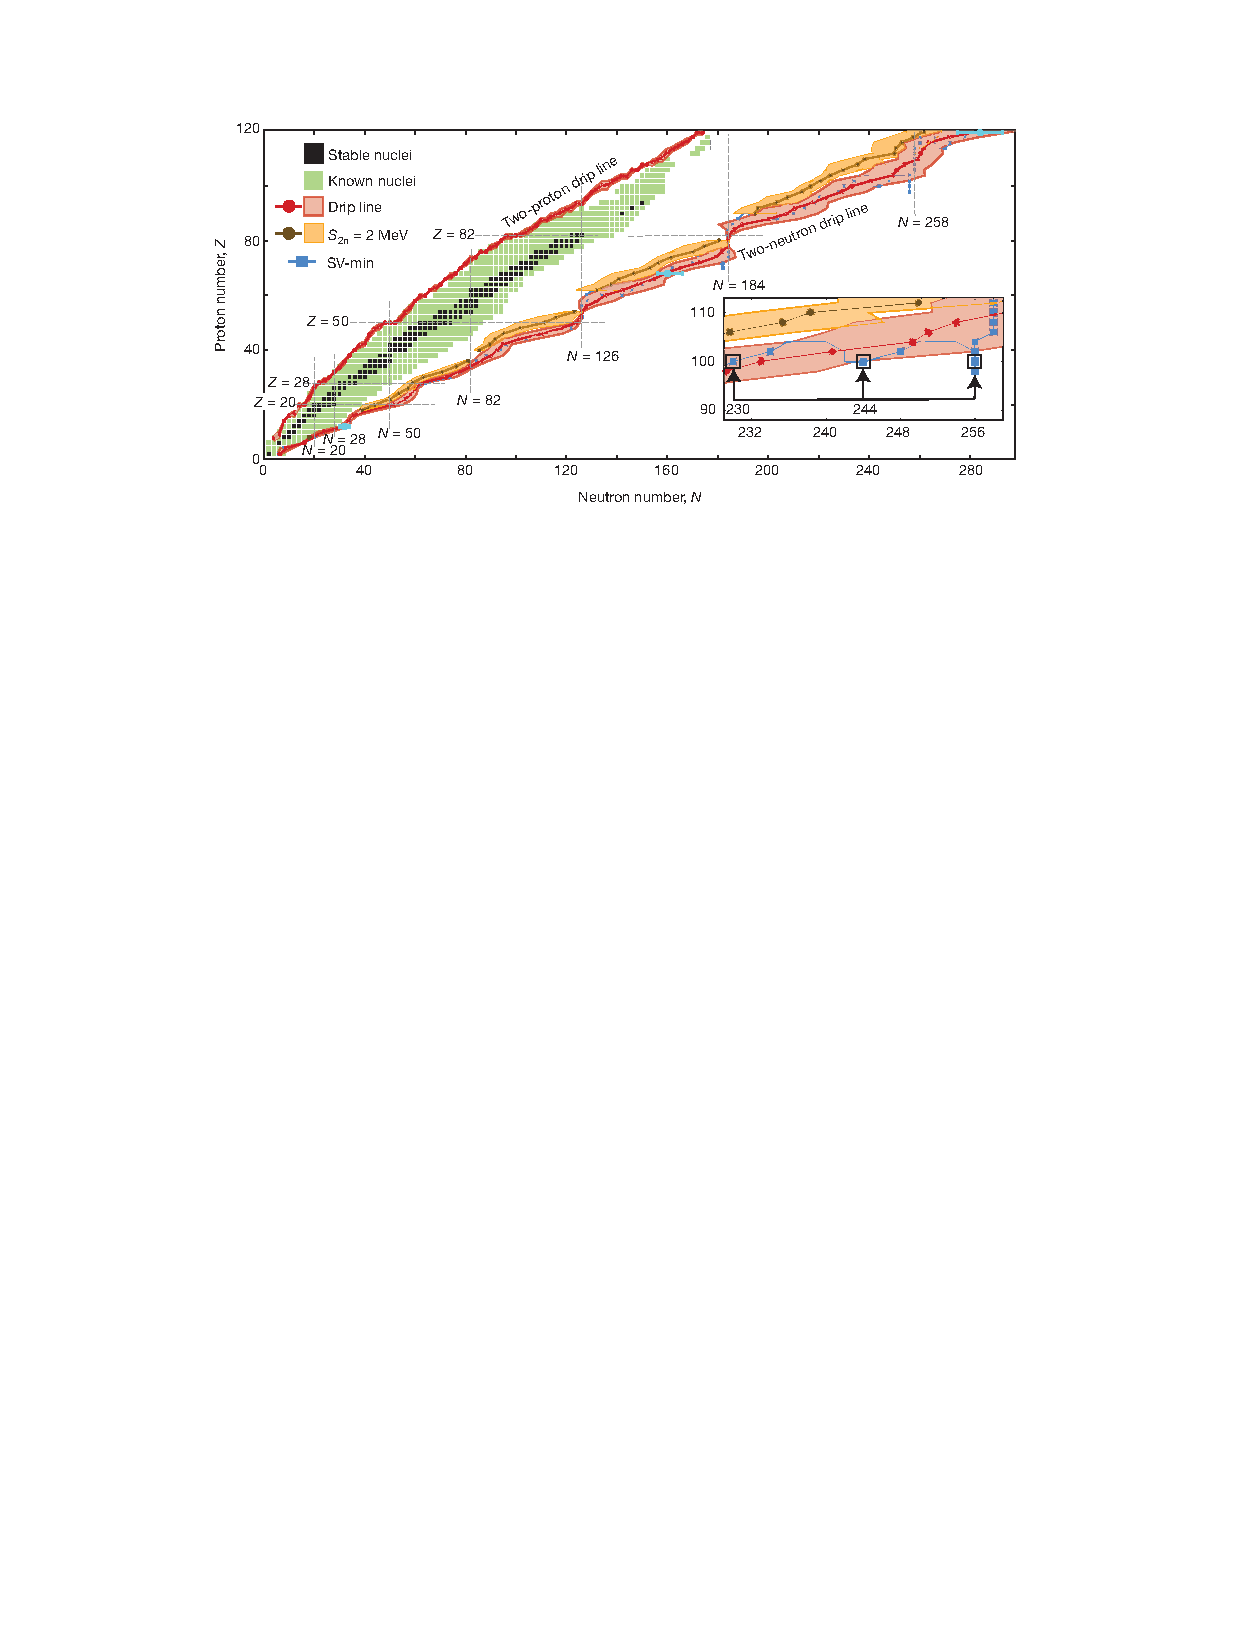
\includegraphics[width=1.0\textwidth]{thesis/doc/images/external/nuclear_landscape_embedded.pdf}
  \caption[
    The nuclear landscape,
    with stable and unstable atomic nuclei denoted by the black and green squares, respectively,
    and a theoretical prediction of the limit of bound nuclei indicated by the red bands.
  ]{
    The nuclear landscape,
    with stable and unstable atomic nuclei denoted by the black and green squares, respectively,
    and a theoretical prediction of the limit of bound nuclei indicated by the red bands.
    Figure taken from Ref.~\cite{Erle12limits}.
  }\label{fig:nuclear_landscape}
\end{figure}

Atomic nuclei consist of protons and neutrons, collectively referred to as nucleons.
The interaction between nucleons is dominated by the strong interaction,
and nuclei as self-bound systems of nucleons form as the result of the strong interaction
overcoming a strong kinetic repulsion
due to nucleons being fermions and obeying the Pauli exclusion principle.
Emergent out of the interplay between these two effects,
with contributions from the weak and electromagnetic interactions,
is the nuclear landscape,
shown in Fig.~\ref{fig:nuclear_landscape}.
All of these isotopes arise out of the same basic physics,
with constituent nucleons interacting via basic two- and three-particle interactions.

\textit{Ab initio} nuclear theory aims to realize this understanding of the nuclear landscape
in theoretical calculations,
determining first the interactions between nucleons
in a way that is connected to the fundamental theory of the strong interaction
and then
modeling nuclei using only the interactions between nucleons as input.
Using only these interactions as inputs means that \abinitio{} methods
have far-reaching predictive power with a large range of applicability.
An additional requirement for the \abinitio{} approach is that
the methods used are in a theoretical limit exact
and thus systematically improvable for any practical approximation.
This feature also allows the \abinitio{} approach to in principle deliver robust uncertainty estimates,
allowing for the meaningful comparison between experiment and theory
and also between different \abinitio{} theoretical approaches.

\begin{figure}[t]
  \centering
  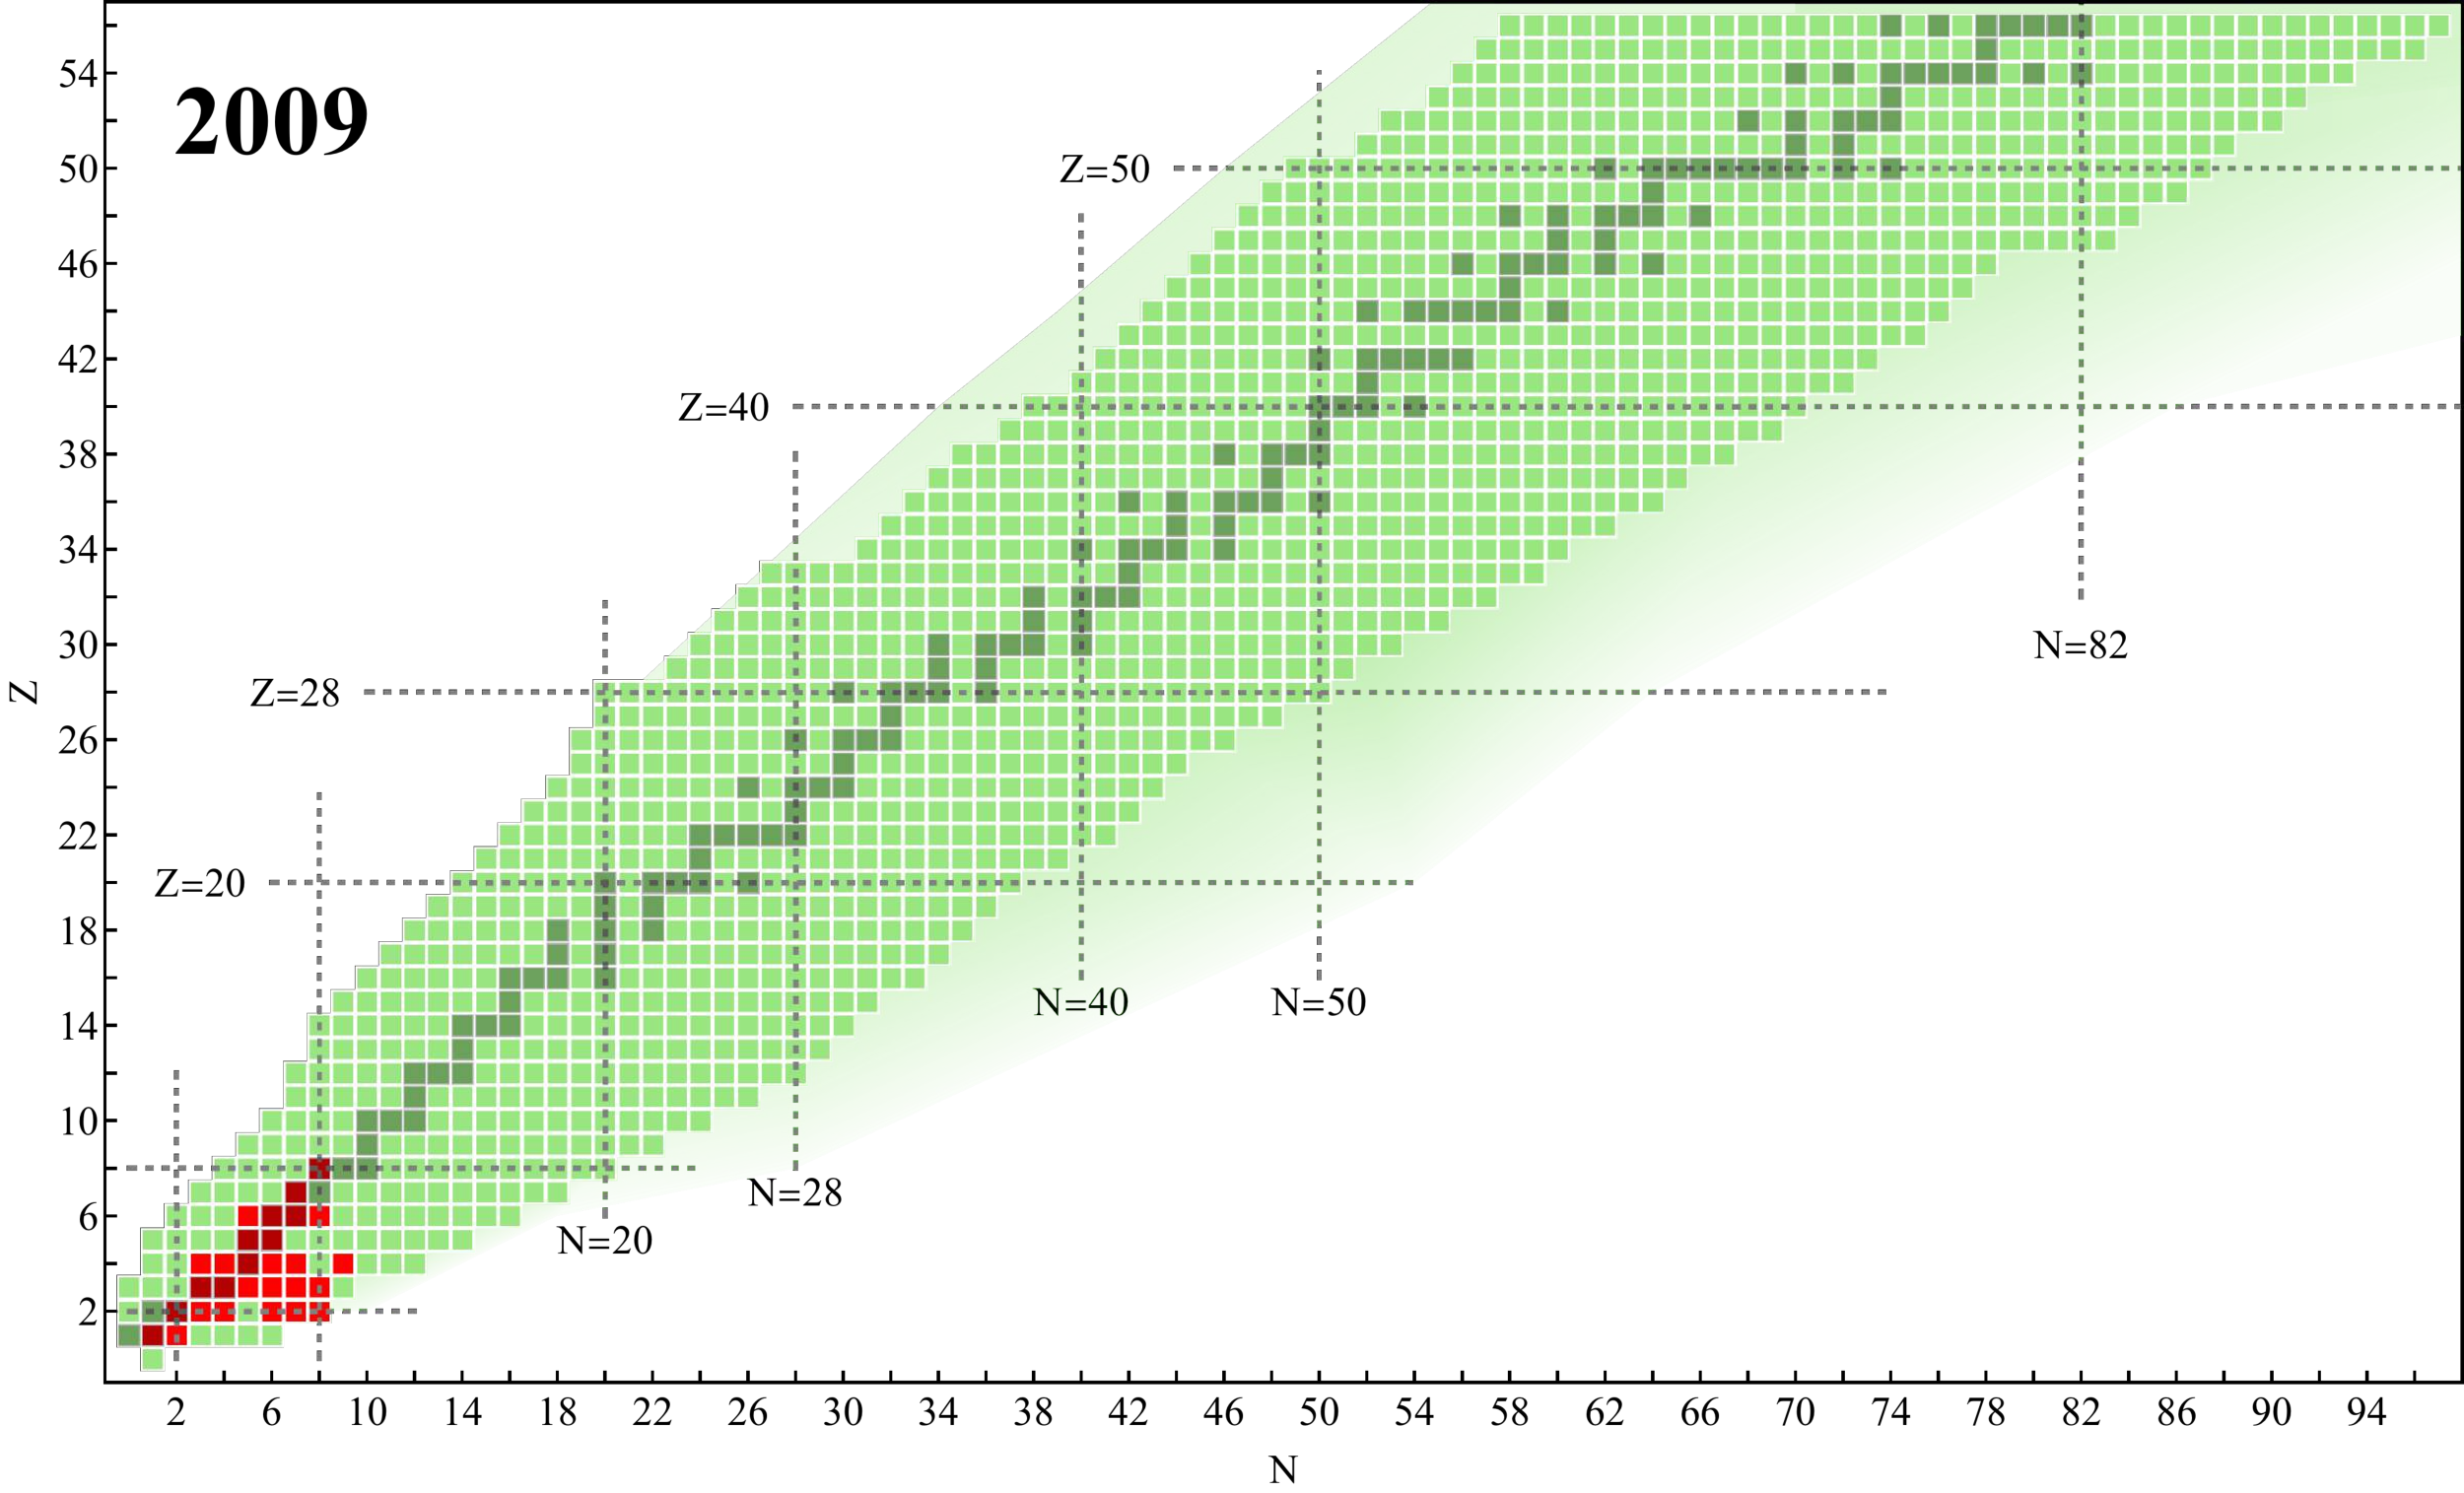
\includegraphics[width=0.45\textwidth]{thesis/doc/images/external/nuclear_chart_2009.pdf}
  \hspace{0cm}
  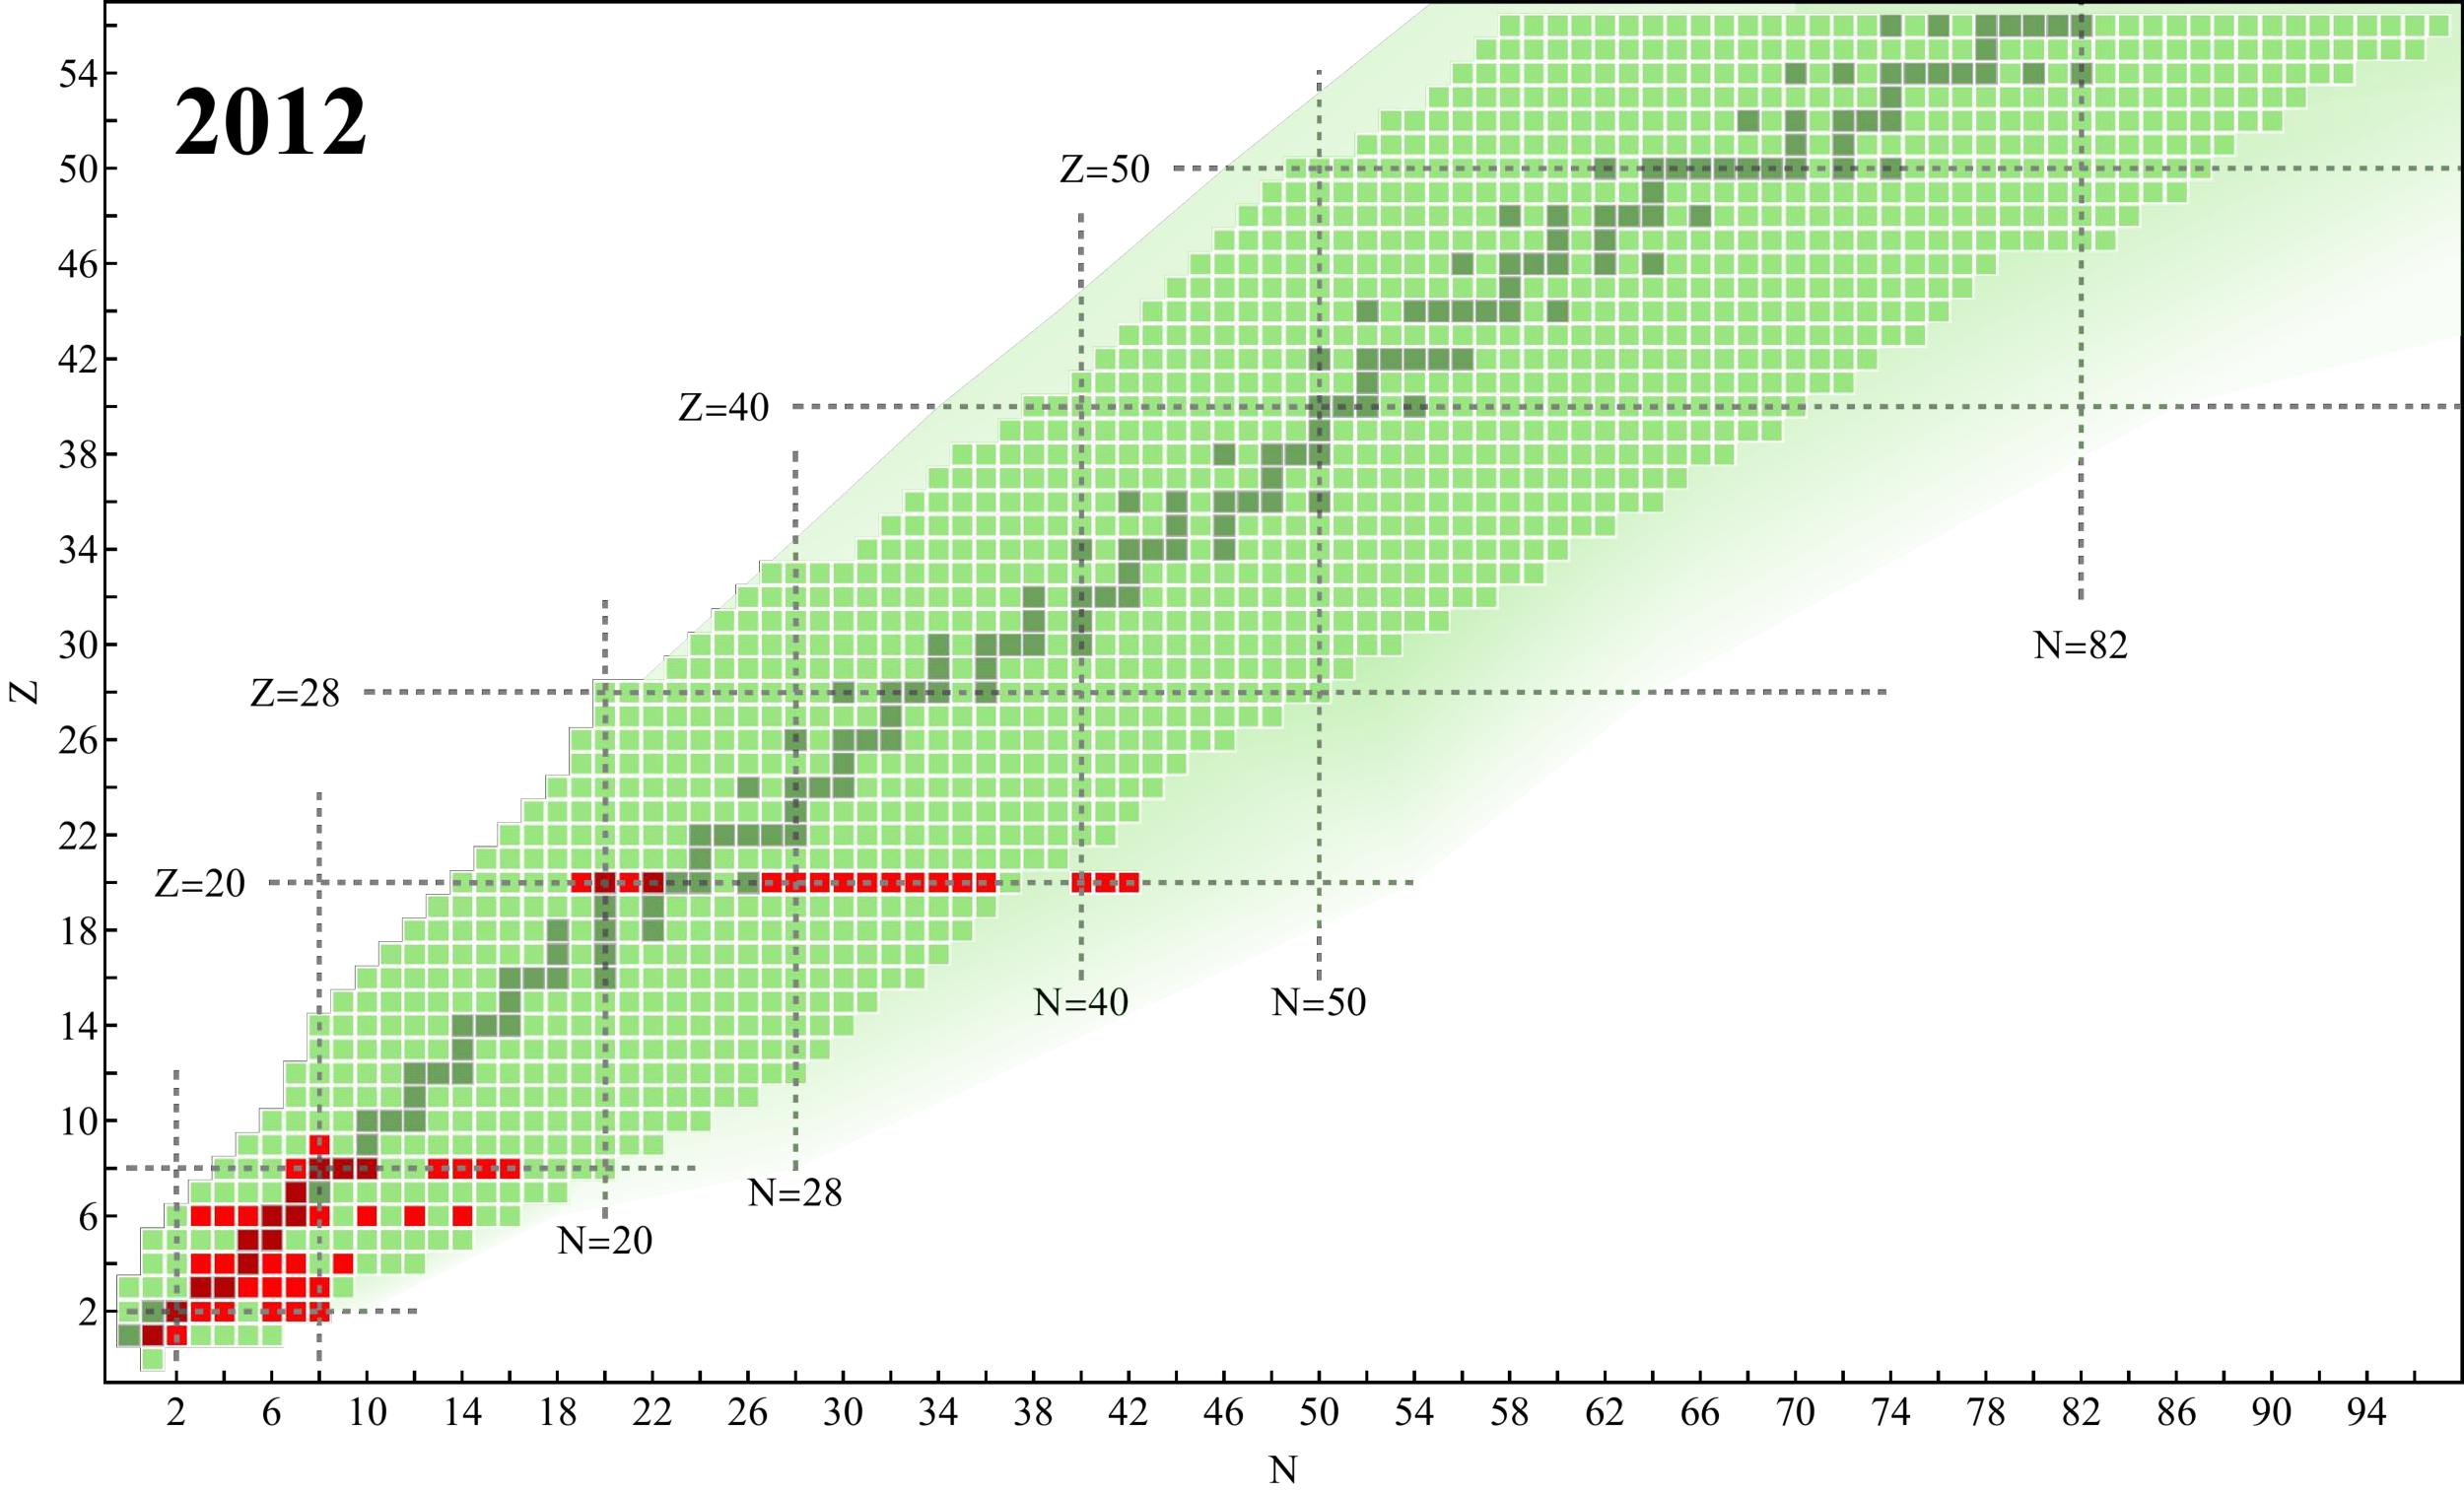
\includegraphics[width=0.45\textwidth]{thesis/doc/images/external/nuclear_chart_2012.pdf}\\
  \vspace{0.05cm}
  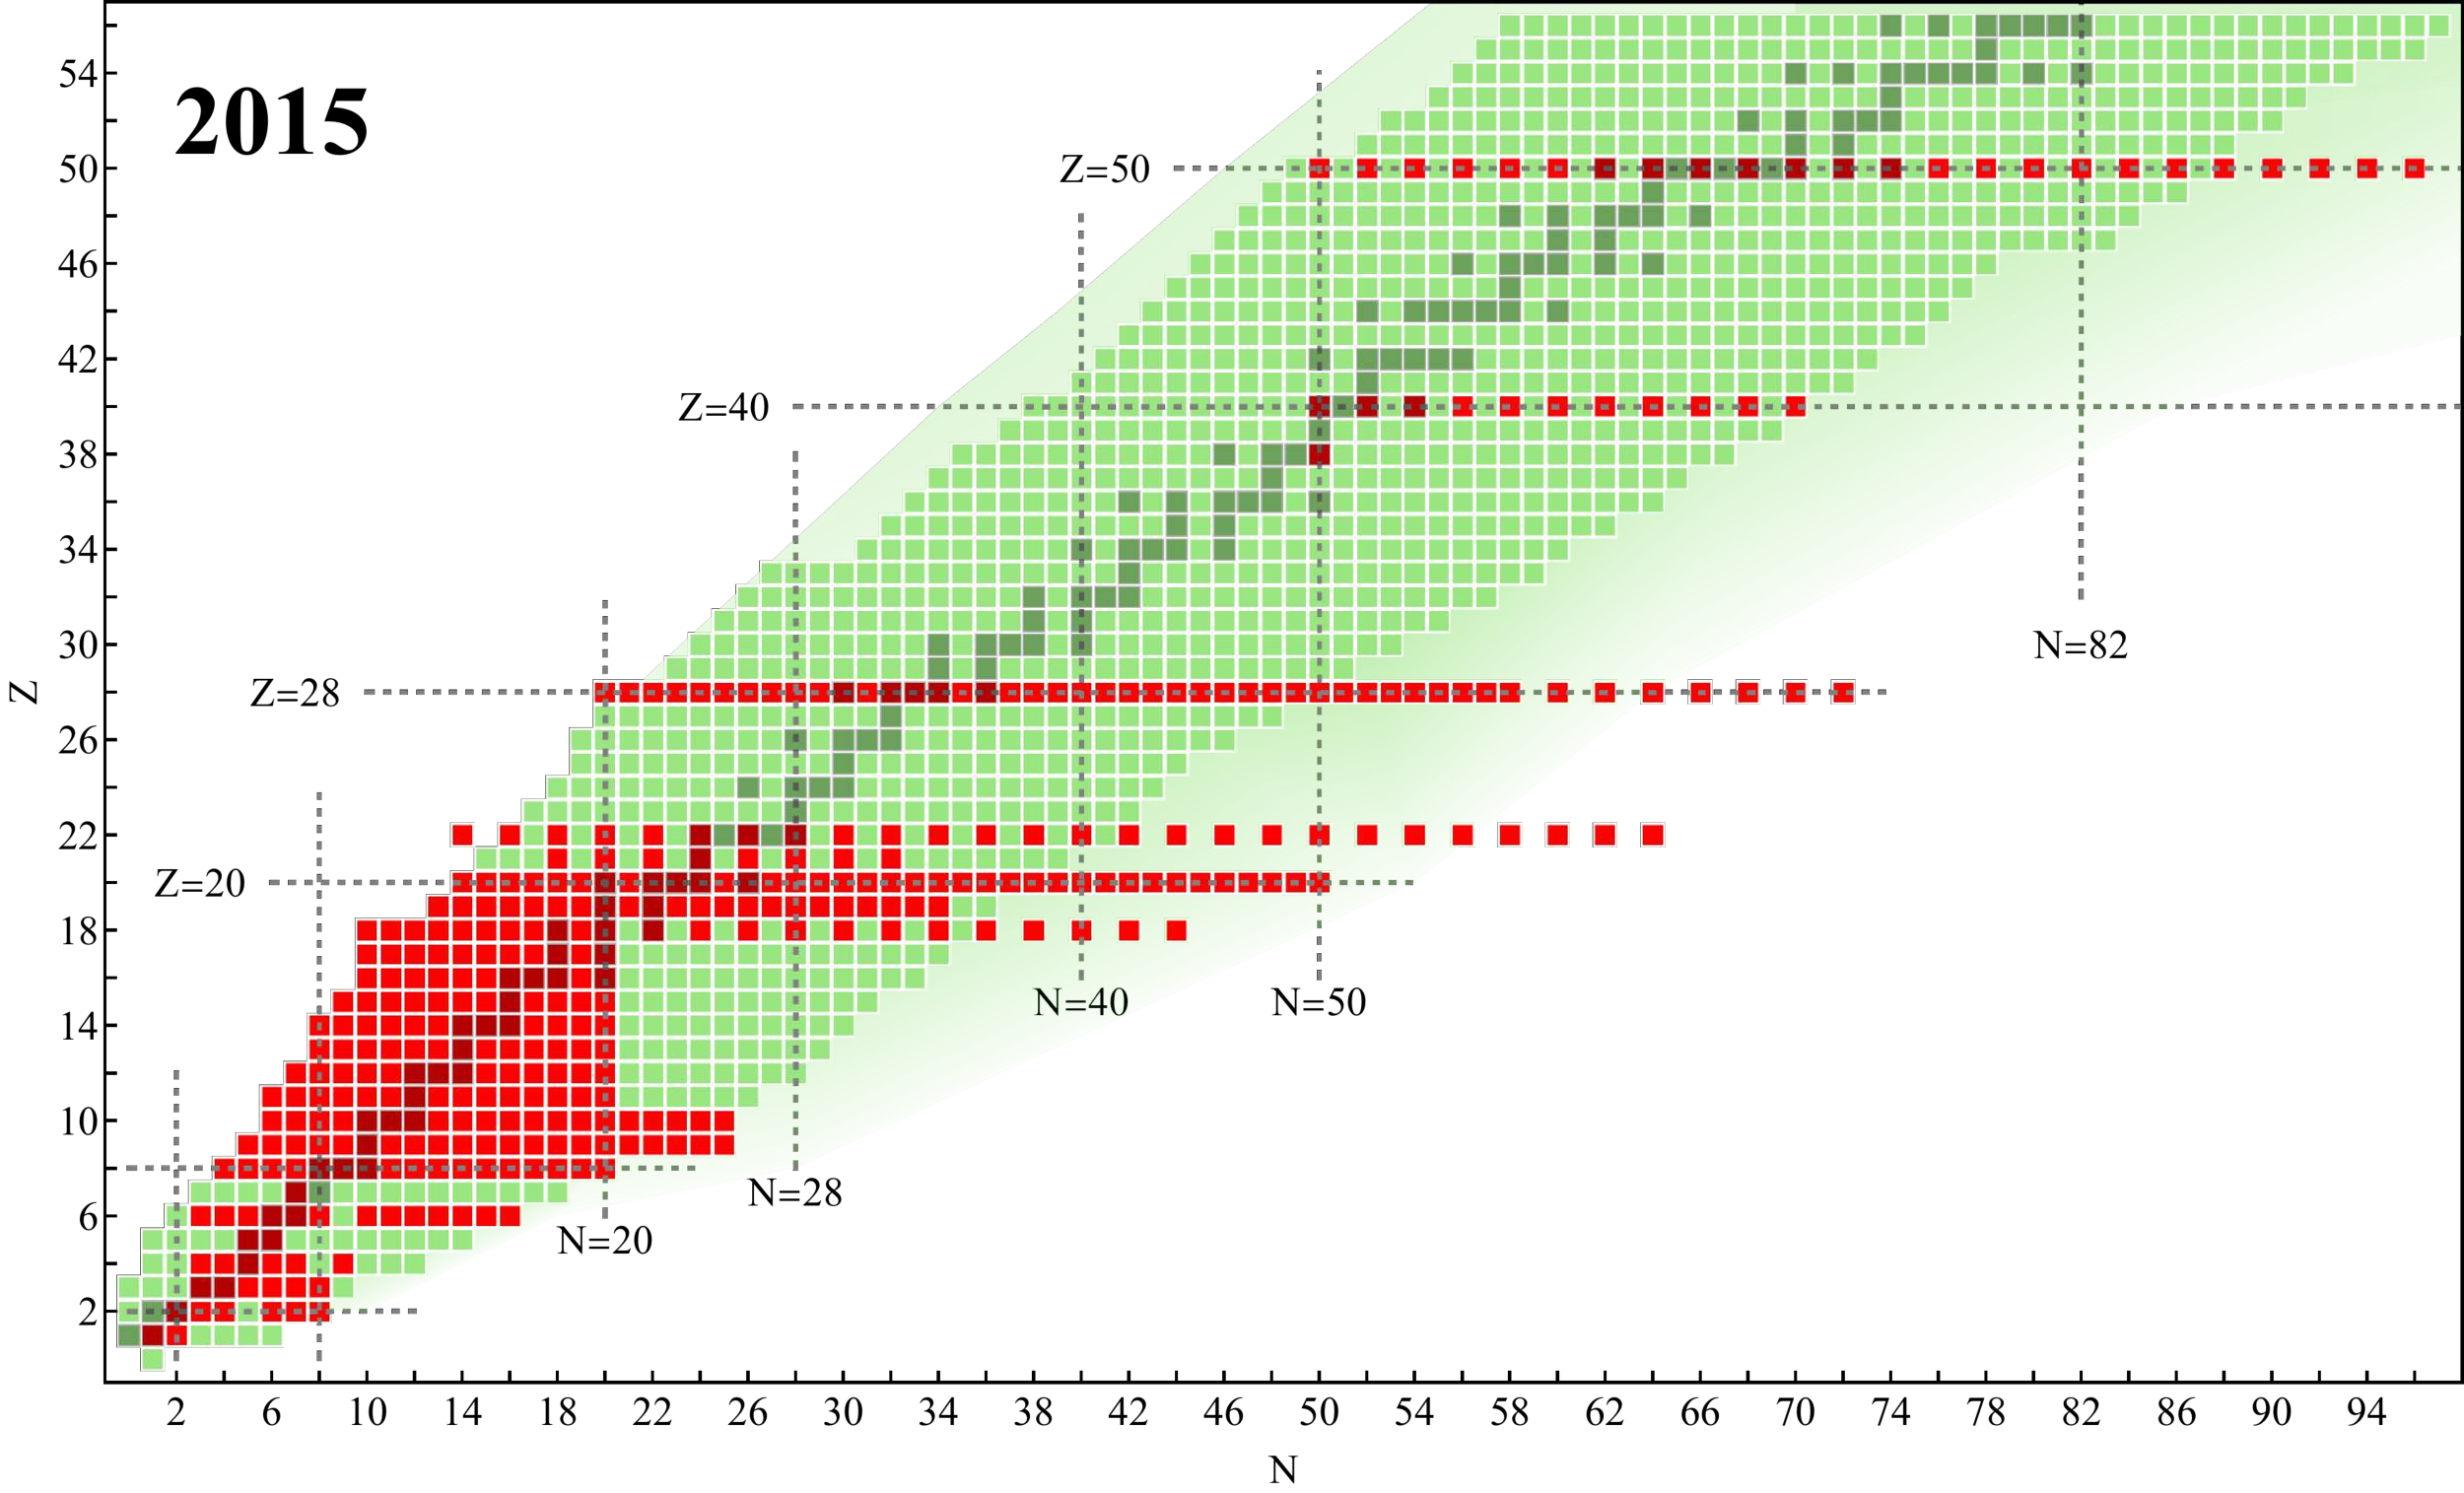
\includegraphics[width=0.45\textwidth]{thesis/doc/images/external/nuclear_chart_2015.pdf}
  \hspace{0cm}
  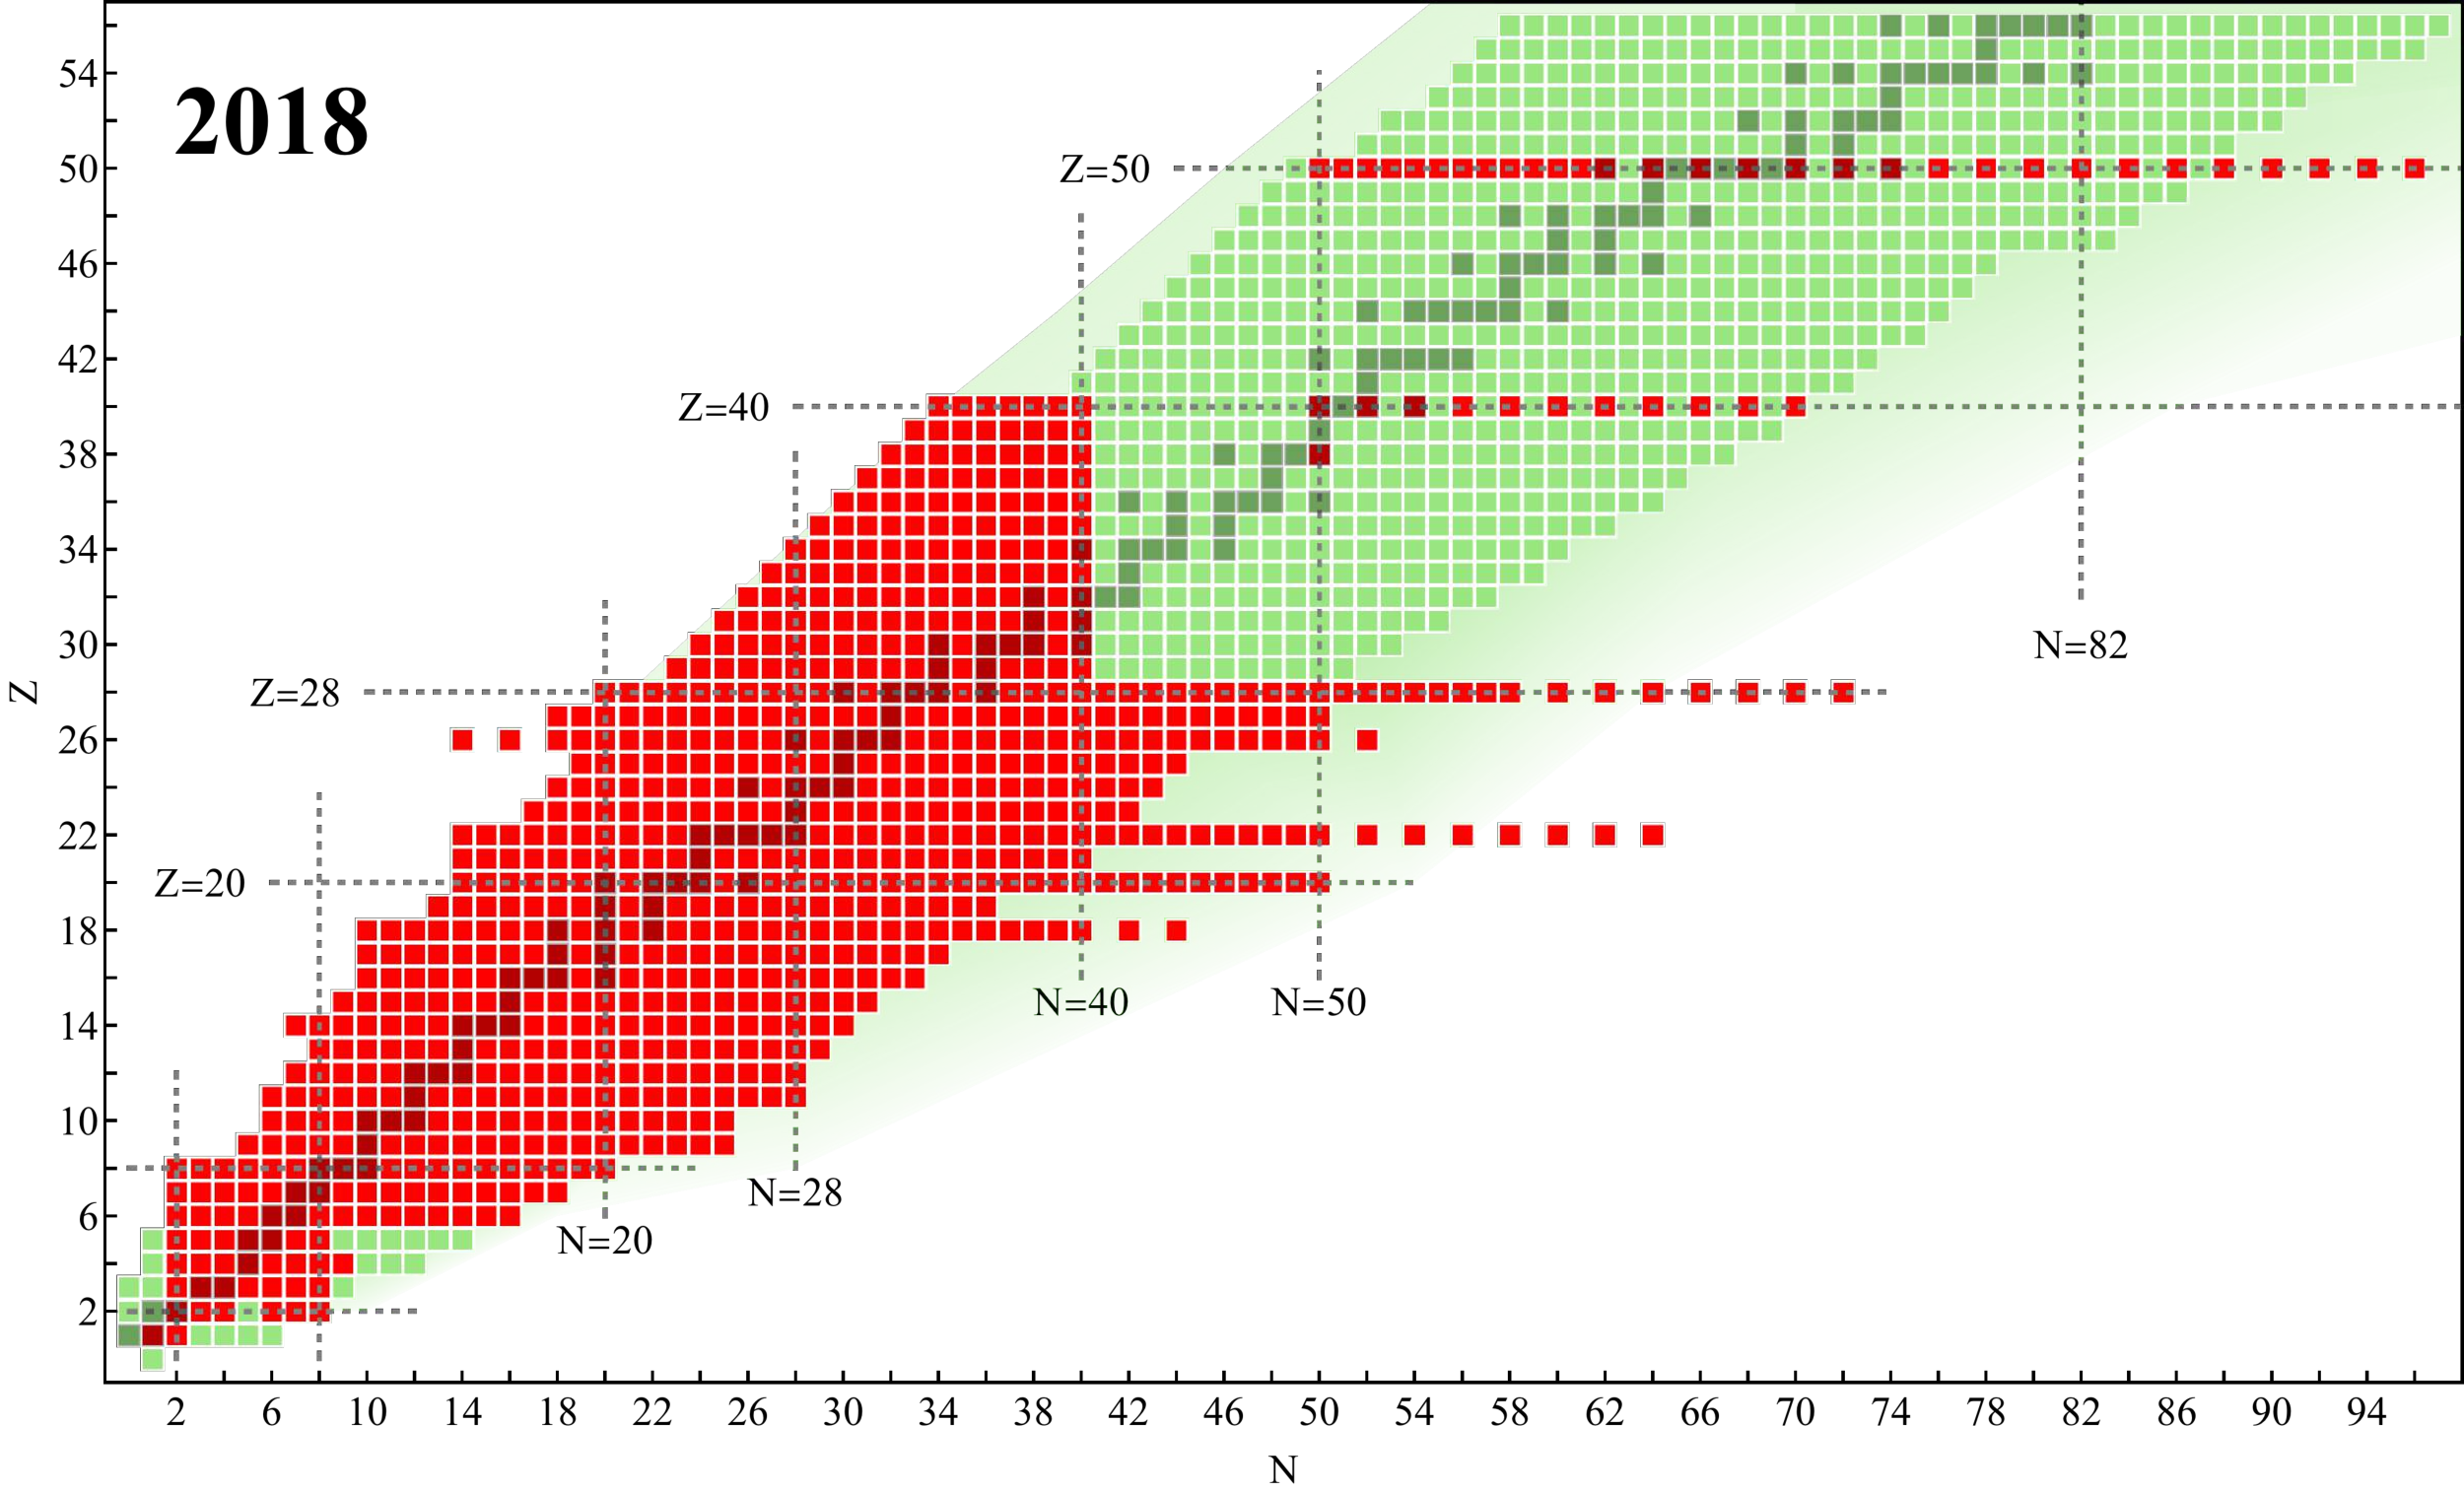
\includegraphics[width=0.45\textwidth]{thesis/doc/images/external/nuclear_chart_2018.pdf}
  \caption[
    Chart of nuclides showing in red nuclei for which \abinitio{} calculations
    involving two- and three-body interactions had been done in 2009 (top left)
    to 2018 (bottom right).
    Only calculations for which convergence with respect to basis size was achieved
    are included in the charts.
  ]{
    Chart of nuclides showing in red nuclei for which \abinitio{} calculations
    involving two- and three-body interactions had been done in 2009 (top left)
    to 2018 (bottom right).
    Only calculations for which convergence with respect to basis size was achieved
    are included in the charts.
    Figure courtesy of Heiko Hergert~\cite{Herg15imsrgphysrep}.
  }\label{fig:ab_initio_conquest}
\end{figure}

Over the past two decades,
the range of \abinitio{} results has expanded rapidly,
as is shown in Fig.~\ref{fig:ab_initio_conquest}.
This change was driven by a shift in our understanding of \textit{low-energy}
nuclear physics,
both in the determination of nuclear interactions
and in the subsequent modeling of nuclei.
The essential change in our understanding of nuclear forces
is encapsulated in the effective field theory (EFT) and renormalization group (RG) methods.
Underlying both of these ideas is the concept of limited resolution in low-energy physics
and the realization that behavior at short distances (small wavelengths or high energies)
does not affect the big picture at long distances.
Effective field theory methods connect to underlying fundamental theories
explicitly setting the scale to include essential long-distance physics
and generating the most general expansion for the short-distance physics
in terms of contact interactions~\cite{Wein78eft,Hamm19nuceftreview,Epel08chiraleft,Mach11chiraleft}.
Renormalization group methods allow for varying of the resolution scale,
decoupling or integrating out high-energy details to produce an efficient low-resolution
description of the system at hand~\cite{Wils71rg,Bogn06srg,Bogn09vlowk}.
These two obviously synergistic methods have worked together to produce
low-resolution nuclear forces rooted in the fundamental theory of quantum chromodynamics.

With these new, more efficient low-energy nuclear forces
and the ever increasing available computational resources,
the parallel development of nuclear many-body methods was uncapped.
New developments on well-established methods,
such as the coupled cluster approach,
and the introduction of new methods,
such as the in-medium similarity renormalization group,
have carried \abinitio{} nuclear theory to its present state.
A crucial role was played by the developments on
many-body expansion methods, such as coupled cluster or
the in-medium similarity renormalization group,
whose computational cost scales polynomially
in the system size
rather than exponentially like
exact diagonalization approaches
or Monte Carlo simulations.
These methods are the best candidates available
for extending the reach of \abinitio{} nuclear theory
to the heavy-mass region
and the neutron-rich medium-mass region.

\section{Goals}

The focus of this work is the in-medium similarity renormalization group (IMSRG)~\cite{Tsuk10imsrg}.
As indicated by its name,
it brings the RG approach of decoupling low- and high-energy states to the many-body problem,
seeking to decouple the state of a system from its elementary excitations.
It is flexible in that it can target both ground states and low-lying excited states
and calculate energies as well as expectation values for other operators,
and while its original formulation centers on describing closed-shell nuclei,
multiple variants are able to model open-shell nuclei
as well~\cite{Stro16vsimsrg,Bogn14vsimsrg,Herg2013mrimsrg,Gebr2016imncsm,Yao18imgcm}.

The current state-of-the-art IMSRG approaches truncate the formalism at the IMSRG(2) level,
the first non-trivial truncation where up to normal-ordered two-body operators are kept in the equations.
This truncation has been quite successful,
but for the purposes of reaching higher precision and allowing for quantification
of many-body uncertainties,
extending the truncation to the IMSRG(3) level is of great interest.
In practice, the general IMSRG(3) is computationally too expensive to allow for
a systematic study in even the smallest systems and model spaces.
By considering only closed-shell systems,
one can apply spherical symmetry to reduce the IMSRG(3)
based on the shared symmetries of the system, the Hamiltonian, and computational basis.
For the IMSRG, this formulation is less restrictive than one may expect,
as the valence-space IMSRG can be used to produce an effective shell-model Hamiltonian
that can be fed into a shell-model code and predict the properties of open-shell nuclei
as well~\cite{Bogn14vsimsrg,Stro16vsimsrg,Holt19vsimsrg_range}.
In this work, we perform the angular-momentum reduction of the IMSRG(3).
We aim to use this to systematically study the improvements offered by the IMSRG(3)
for the ground-state properties of light and medium-mass nuclei.

\section{Outline}

The remainder of this thesis is structured as follows:
\begin{itemize}
  \item{In Chapter~\ref{ch:nuclear_forces},
        we introduce some aspects of the theory of nuclear forces.
        We focus on the modern approaches to deriving nuclear forces
        and
        the construction and generation of low-resolution Hamiltonians
        that improve the convergence of many-body calculations.}
  \item{In Chapter~\ref{ch:many_body},
        we introduce the many-body formalism that underlies the IMSRG.\@
        We introduce some related many-body methods that also build on this formalism
        to help position the IMSRG in the greater space of available many-body methods.}
  \item{In Chapter~\ref{ch:imsrg},
        we discuss the IMSRG in detail.
        We discuss the general formalism and the IMSRG(2) and IMSRG(3) truncations.
        We also discuss generator choice,
        which sets how the IMSRG decouples low and high energies,
        and the Magnus expansion,
        an extension that makes the IMSRG easier to solve and easier to apply to other observables.
        We show some benchmark results for our implementation of the IMSRG(2) for ${}^4\text{He}$.}
  \item{In Chapter~\ref{ch:ang_mom_coupling},
        we introduce the angular-momentum reduction formalism.
        We apply this formalism to the IMSRG(3)
        and some auxiliary many-body operations.
        The result is the IMSRG(3) in a spherically symmetric basis,
        which is computationally more efficient
        and allows us to solve the flow equations
        for light and medium-mass nuclei in small model spaces.}
  \item{In Chapter~\ref{ch:jscheme_results},
        we discuss the contributions of the IMSRG(3) truncation
        to ground-state properties of nuclei
        using the optimized spherically-reduced IMSRG(3).
        We consider how the IMSRG(3) handles different reference state choices,
        and we investigate what the effects of individual contributions to the IMSRG(3) are.}
  \item{In Chapter~\ref{ch:summary},
        we summarize our results
        and offer an outlook for the next steps
        in exploring three-body effects in the IMSRG.}
\end{itemize}


\chapter{Nuclear forces}\label{ch:nuclear_forces}

For low-energy nuclear physics,
the goal is to understand the structure and dynamics of systems
with nucleons as constituents.
Thus, a key input into any theoretical calculations of such systems
is the interactions between nucleons.
However, quantum chromodynamics (QCD),
the theory of the strong interaction,
is given in terms of quarks and gluons, not nucleons.
Moreover, at low energies the strong interaction coupling constant $\alpha_s(q^2)$ becomes large,
preventing a fundamental closed-form solution for the interactions between color-neutral hadrons.

As a result, various approaches to determining the interactions between nucleons
have been developed.
One such approach is the phenomenological expansion of the interaction between two nucleons
into terms with different spin, isospin, and angular-momentum dependences.
The (position- and momentum-dependent) strength of each of these terms is then fit to nucleon-nucleon scattering data,
giving rise to, for example, the AV18 potential~\cite{Wiri95AV18}.
This approach has several features that make it undesirable for \abinitio{} nuclear theory.
First, it does not connect to the underlying fundamental theory.
Second, this approach does not prescribe a way to arrive at consistent three-nucleon forces.
Additionally, the fitting procedure often includes scattering data at relatively high energies
when compared to the expected kinetic energy of nucleons in nuclei or nuclear matter,
making such phenomenological interactions highly non-perturbative.

In this chapter, we discuss chiral effective field theory
as an alternative to the phenomenological determination of nuclear forces
and the similarity renormalization group as a method to generally ``soften'' interactions
for many-body calculations.
Then we discuss some details regarding different bases
in which one can represent nuclear potentials.

\section{Nuclear forces from chiral effective field theory}

\begin{figure}[t!]
  \centering
  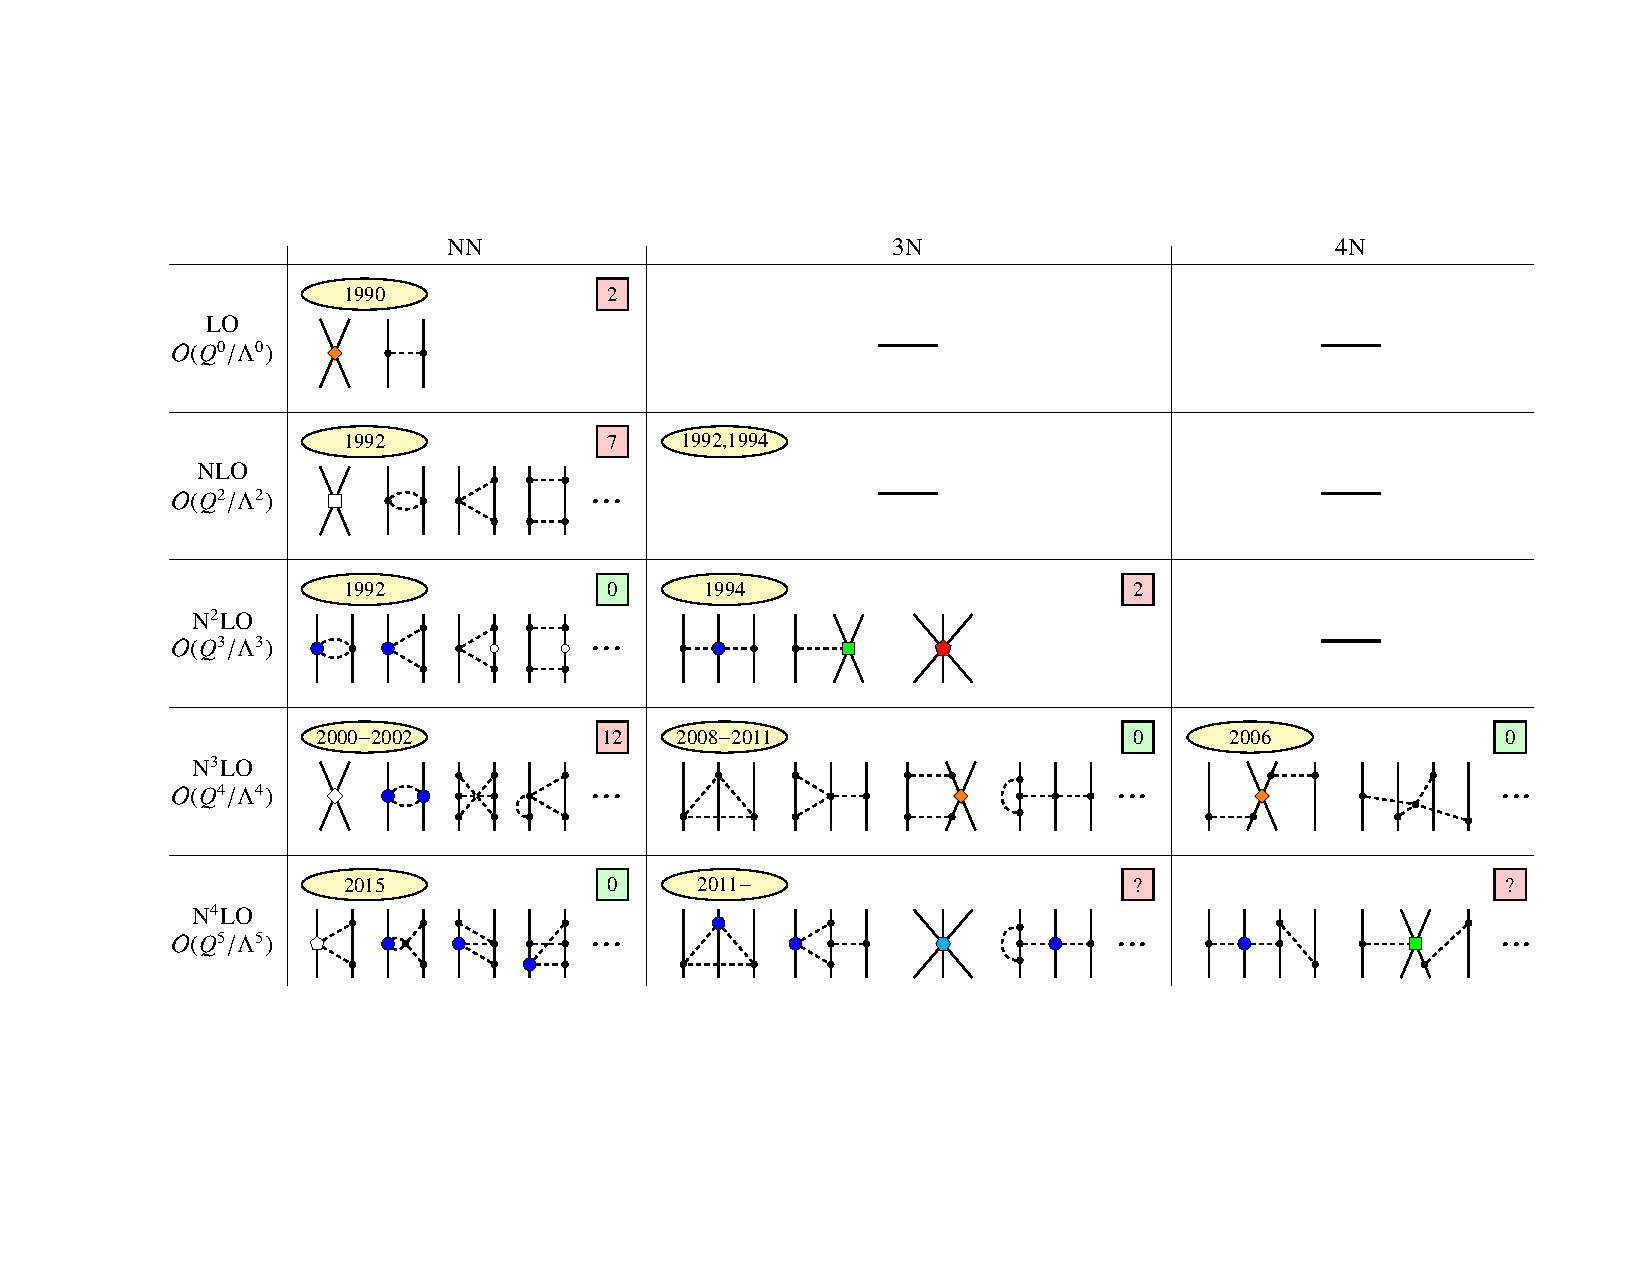
\includegraphics[width=1.0\textwidth]{thesis/doc/images/external/table_norefs.pdf}
  \caption[
    The contributions to NN, 3N, and 4N interactions in chiral EFT
    up to order \nfourlo{}.\@
    Solid lines indicate nucleon propagators.
    Dashed lines indicate pion propagators.
    The number of new LECs for the new interaction contributions at each new order
    is shown in the top right corner.
  ]{
    The contributions to NN, 3N, and 4N interactions in chiral EFT
    up to order \nfourlo{}.\@
    Solid lines indicate nucleon propagators.
    Dashed lines indicate pion propagators.
    The number of new LECs for the new interaction contributions at each new order
    is shown in the top right corner.
    Figure taken from Ref.~\cite{Hebe20habi}.
  }\label{fig:chiefttable}
\end{figure}

A modern approach to deriving nuclear potentials is chiral effective field theory.
The EFT approach allows one to systematically construct a field theory that approximates
a more fundamental theory in a low-energy domain~\cite{Epel08chiraleft,Mach11chiraleft,Hamm19nuceftreview}.
In this apppropriately chosen domain,
one can use the most efficient degrees of freedom to formulate the theory.
The construction of the theory relies on knowing the symmetries (exact and approximate) of the underlying theory.
Constructing the most general Lagrangian consistent with these underlying symmetries
yields the most general $S$-matrix~\cite{Wein78eft}.

To construct an effective field theory, one identifies the degrees of freedom one wants to work with
and identifies a high-momentum scale $\Lambda$ of the underlying theory that characterizes physics no longer resolved by the EFT~\cite{Hamm19nuceftreview}.
The EFT then should be an efficient, approximately complete description of the relevant physics
at momenta $Q$ small compared to $\Lambda$.
The chosen degrees of freedom are used to construct the most general Lagrangian consistent with the underlying symmetries,
which will have an infinite number of terms each with their own coefficients,
the so-called low-energy constants (LECs).
The EFT can then be used to calculate observables up to some precision in an expansion in $Q/\Lambda$,
made systematic by a power-counting approach.

For chiral EFT,
the underlying theory is QCD in the light-quark sector
(here this means only up and down quarks),
where the Lagrangian has an approximate chiral symmetry $\text{SU}{(2)}_L \times \text{SU}{(2)}_R$
in the limit of vanishing quark masses and no electroweak interactions~\cite{Hamm19nuceftreview}.
This symmetry is spontaneously broken,
giving rise to the pion as the Goldstone boson associated with the broken $\text{SU}{(2)}_A$ symmetry,
as well as explicitly broken by the non-zero quark masses~\cite{Page74chisymm}.
A logical choice of degrees of freedom is then nucleons and pions.
The high-momentum scale $\Lambda_b$ is set by the lightest meson not included in our degrees of freedom,
the $\rho$ meson with a mass of $m_{\rho}\approx 770 \mev$~\cite{Mach11chiraleft}.
The low-momentum scale is a collective scale given by $\text{max}(Q, m_{\pi})$.

The resulting potential contributions from chiral EFT have either explicit pion exchanges
or contact interactions with LECs describing short-range physics unresolved by the EFT,
as shown in Fig.~\ref{fig:chiefttable}.
The first consistent three-nucleon (3N) interactions appear at next-to-next-to-leading order (\ntwolo{}),
and the first four-nucleon (4N) interactions appear at next-to-next-to-next-to-leading order (\nthreelo{}).
Among the features that make EFTs so powerful is that they allow for clear error estimates~\cite{Furn15bayesuq,Epel14ekm1,Epel14ekm2},
given proper power counting,
by considering the order-by-order convergence of observables
and seeing that the orders left out due to a truncation at order $N$ should contribute something like
\begin{equation}
  \Delta O^{(N)} \sim O {\left(\frac{\text{max}(Q, m_{\pi})}{\Lambda_b} \right)}^{N+1}\,,
\end{equation}
where $O$ is the exact result for some observable of interest
(see Fig.~\ref{fig:chieft_uq}).

For potentials from chiral EFT,
at each order a finite number of undetermined LECs are introduced with the new contributions to the potential.
For nucleon-nucleon (NN) interactions, these can be determined by fitting to \textit{low-energy} scattering data.
For 3N interactions, the relevant LECs must be fit to three-body or four-body observables.
Typical choices for these observables at \ntwolo{}, where two three-body LECs, $c_D$ and $c_E$, need to be fit,
are the triton binding energy and either the triton half-life or the ${}^4\text{He}$ charge radius~\cite{Hebe20habi}.
Additionally, some contributions at later orders in the expansion only depend on LECs from previous orders.
For example, the 3N force contributions at \nthreelo{} require no new LECs to be fit.

\begin{figure}[t!]
  \centering
  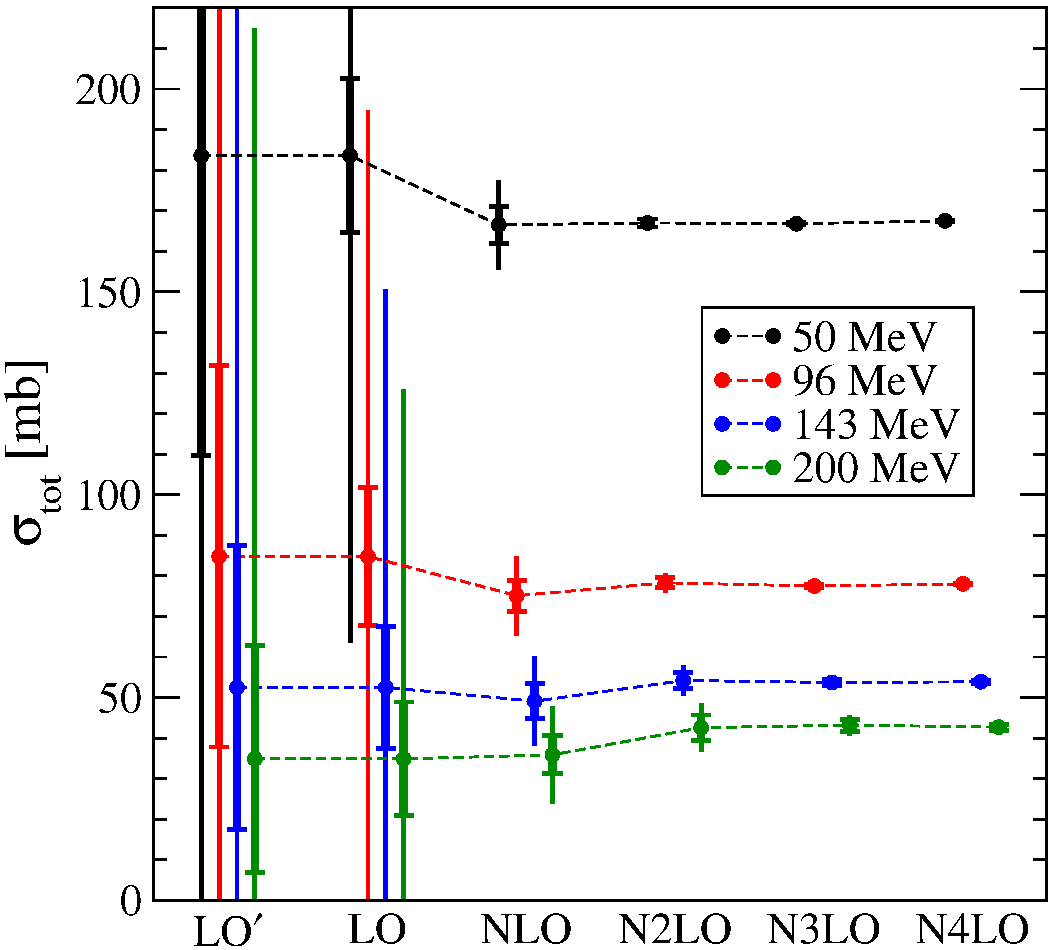
\includegraphics[width=0.5\textwidth]{thesis/doc/images/external/EKM_Tlab_together_setA_eps_approx0.pdf}
  \caption[
    The total proton-neutron scattering cross section
    calculated order by order at different energies
    using chiral potentials
    with 68\% and 95\% degree of belief intervals
    indicated by the thick and thin error bars
    obtained via Bayesian uncertainty quantification.
  ]{
    The total proton-neutron scattering cross section
    calculated order by order at different energies
    using potentials from Ref.~\cite{Epel14ekm2}
    with 68\% and 95\% degree of belief intervals
    indicated by the thick and thin error bars
    obtained via Bayesian uncertainty quantification~\cite{Furn15bayesuq}.
    Figure taken from Ref.~\cite{Furn15bayesuq}.
  }\label{fig:chieft_uq}
\end{figure}

Some comments are now in order regarding interactions as used in this thesis.
The derivation of potentials requires the explicit regularization of momenta
to make divergent integrals over intermediate momenta convergent.
This introduces a dependence on the regularization scheme and scale used,
which is an artifact of the finite order of our EFT.\@
Each additional order in the EFT cancels the scale dependence of the previous order,
and in the limit of infinite order all observables
should not depend on the cutoff scale and scheme used (within reason).
For every interaction used we state the order, the regularization scale,
and the family of interactions, which specifies the regularization scheme used.

We primarily use two families of interactions.
The first set is a family of interactions with NN interactions given up to \nthreelo{},
which was worked out by Entem and Machleidt in 2003~\cite{Ente03n3lonn}.
These interactions are denoted by EM when they are used.
The second set was worked out by Entem, Machleidt, and Nosyk in 2017
and provides NN interactions up to \nfourlo{}~\cite{Ente17n4lonn}.\@
These interactions are denoted by EMN.\@
From 2007 through 2011, the 3N interactions were worked out~\cite{Ishi07chi3n,Bern07chi3n1,Bern11chi3n2},
and the consistent
(in terms of power counting and regularization scheme)
3N potentials with these families up to \nthreelo{}
were presented in 2015 by Hebeler \textit{et al.}~\cite{Hebe15n3lo3n}.
At \nthreelo{}, the chiral power counting dictates the inclusion of 4N forces
(see Fig.~\ref{fig:chiefttable}).
However, this is generally \textit{not} done
because the inclusion of 4N forces in calculations is prohibitively expensive
and past results have shown that they contribute at the sub-1\%
level~\cite{Tews12neutronmatter4n,Schu18fourbody}.

Chiral EFT essentially resolves all of the shortcomings of phenomenological potentials mentioned previously.
There are still many open questions regarding the derivation of potentials via chiral EFT
and their consistent application in many-body calculations.
For example, there are multiple schools of thought regarding
what the correct power counting
for nuclear potentials is~\cite{Bean01pertchieft,Nogg05pertchieft,Epel18hownottorenormalize}.
Additionally, the uncertainties from the regularization scheme and scale for nuclear potentials
are still most likely dominant in many-body calculations.
However, the rapid expansion of the range of \abinitio{} calculations over the past two decades has been in no small part
due to the introduction of chiral potentials and the development of auxiliary tools to aid in their application
to many-body calculations.

\section{Similarity renormalization group evolution of nuclear forces}\label{sec:srg}

The similarity renormalization group (SRG) is a method that has been used to great success to ``soften'' nuclear interactions~\cite{Bogn06srg,Wegn94srg,Glaz93srg}.
The key idea of the SRG is the generation of a continuous unitary transformation of a given Hamiltonian $H$,
\begin{equation}
  H(s) = U(s) H U^{\dagger}(s)\,,
\end{equation}
where $s$ is the continuous flow parameter.
The resulting flow equation gives the evolution of the Hamiltonian
\begin{equation}\label{eq:srg_flow_eq}
  \frac{d H(s)}{ds} = [\eta(s), H(s)]\,,
\end{equation}
with $\eta(s) = U(s) d U^{\dagger}(s)/ ds$ and we choose $H(0) = H$.
An ``appropriate'' choice of the anti-Hermitian generator $\eta$
can generate a unitary transformation
such that $H(s)$ evolves, for example, towards a diagonal form.
This leads to a decoupling of low- and high-energy states in the Hamiltonian,
allowing for a truncation in momentum space or a discretized basis
without distorting low-energy observables.

The evaluation of the commutator in the SRG flow equation generates higher-body forces in the evolved Hamiltonian,
even if the initial Hamiltonian consists only of two- and three-body forces.
This means that the fully unitary SRG evolution of an $A$-body Hamiltonian
requires the evaluation of the flow equation in the $A$-body basis.
For all but the smallest systems, this is computationally infeasible.

A pragmatic approach uses the SRG restricted to the three-body space
to evolve two- and three-body nuclear forces to ``softer'' forms in momentum space~\cite{Hebe12srg3n},
reducing coupling between low- and high-energy states.
These evolved potentials are for few-body purposes equivalent to the un-evolved ones,
reproducing the few-body binding energies, radii, and NN phase shifts exactly.
After truncating the potentials, taking advantage of the decoupling,
the few-body observables remain essentially unchanged,
and the low-energy NN phase shifts are also preserved.

The typical choice for the generator in the so-called ``free-space'' SRG in nuclear applications is
\begin{equation}
  \eta(s) = [T_{\text{rel}}, H(s)]\,,
\end{equation}
where $T_{\text{rel}}$ is the relative kinetic energy of the two- and three-body systems.
In two-body Jacobi momentum coordinates, $T_{\text{rel}}$ is diagonal,
thus the right-hand side of the flow equation clearly has a fixed point if $H(s)$ is ever diagonal.
Evaluating the flow equation in momentum space in the two-body case for this choice for $\eta$ gives
\begin{equation}
  \frac{dV_2(s; p, p')}{ds} = - {(p^2 - {p'}^2)}^2 V_2(s; p, p') + \int dp'' (p^2 + {p'}^2 - 2 {p''}^2) V_2(s; p, p'') V_2(s; p'', p')\,,
\end{equation}
where $p$ and $p'$ are the incoming and outgoing Jacobi momenta of the two-body subsystem
(see Section~\ref{sec:jacobi_ms_rep}).
We also used the conventional choice of leaving the kinetic energy invariant under the SRG evolution.
Empirically, one can see that the first term dominates the evolution for far off-diagonal elements in nuclear applications,
and so
\begin{equation}
  V_2(s; p, p') \approx V_2(0; p, p') \exp(- s {(p^2 - {p'}^2)}^2)\,.
\end{equation}
Using a redefinition of the flow parameter
\begin{equation}
  \lambda = \frac{1}{s^{1/4}}\,,
\end{equation}
which has units of $\text{fm}^{-1}$ and evolves from $\lambda=\infty$ towards 0,
one can see that over the course of the evolution
off-diagonal parts of the potential outside a band of width $\lambda$ begin to be exponentially suppressed~\cite{Jurg07srgdec}.
Looking at Fig.~\ref{fig:srg_evolved_potential}, one can see that this is qualitatively true,
and the desired decoupling between low- and high-momentum states is achieved.

\begin{figure}[t]
  \centering
  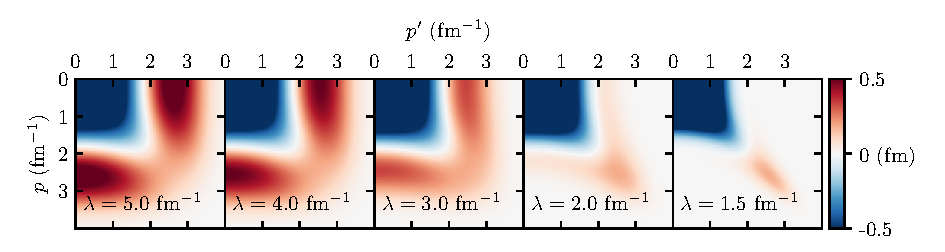
\includegraphics[width=\textwidth]{thesis/doc/images/vnn_srg_emn500_n3lo.pdf}
  \caption[
    An example of an SRG-evolved potential using the chiral EMN NN potential
    at \nfourlo{}
    in the ${}^3$S${}_1$ part of the ${}^3$S${}_1$-${}^3$D${}_1$ channel.
  ]{
    An example of an SRG-evolved potential using the chiral NN potential
    from Ref.~\cite{Ente17n4lonn} at \nfourlo{}
    in the ${}^3$S${}_1$ part of the ${}^3$S${}_1$-${}^3$D${}_1$ channel.
  }\label{fig:srg_evolved_potential}
\end{figure}

These softened interactions can then be fed into many-body frameworks,
which benefit strongly from the improved convergence with respect to model-space size.
However, the few-body evolution of potentials neglects induced $A$-body forces,
which do contribute in many-body calculations.
One way to probe the size of the missing many-body forces is to do calculations
with potentials evolved to different values of $s$ or $\lambda$
and see how much the calculated result depends on the renormalization scale.
A strong dependence would indicate significant missing contributions from many-body forces
while no dependence would indicate approximate renormalization group invariance,
which is ultimately the goal~\cite{Bogn09vlowk}.

\section{Representations of nuclear potentials}

The efficient representation of nuclear potentials exploits symmetries of the few-body system and the interactions.
In particular, for 3N forces,
where the potential can depend in principle on 18 parameters in momentum space
($\vec{k}_1$, $\vec{k}_2$, $\vec{k}_3$, $\vec{k}_{1}^{\prime}$, $\vec{k}_{2}^{\prime}$, $\vec{k}_{3}^{\prime}$),
simplifications afforded by these symmetries are essential
to being able to evaluate, store, and calculate with these potentials.

The essential symmetries of the free two- and three-nucleon systems
(from which the potentials are determined)
are~\cite{Hebe20habi}
\begin{itemize}
  \item conservation of the center-of-mass momentum of the system,
  \item independence on the center-of-mass momentum in the nonrelativistic regime,
  \item and rotational invariance.
\end{itemize}
Additionally, one can simplify things dramatically by making the assumption that the masses of all nucleons are the same,
a reasonable assumption given that the mass difference between the proton and neutron is less than a per mille~\cite{Hebe20habi}.
In this approximation in the absence of electroweak interactions,
the NN force would also be independent of isospin projection,
however the Coulomb interaction breaks this isospin charge symmetry.
Also, even without the Coulomb interaction,
the chiral EFT expansion explicitly breaks isospin charge symmetry at higher orders,
a result of it being constructed in a way
that systematically accounts for the breaking of approximate symmetries.

In the following, we discuss some possible representations of NN forces,
going from one of the representations most convenient for the evaluation of potentials
to the representation of choice for the many-body methods discussed in this thesis.
We mention along the way some of the analogous results for 3N forces.
A more thorough treatment of this topic can be found in Ref.~\cite{Hebe20habi}.

\subsection{Jacobi momentum space}\label{sec:jacobi_ms_rep}

Going from single-particle momenta to Jacobi and center-of-mass momenta,
like
\begin{align}
  \vec{k}_1, \vec{k}_2           & \rightarrow \vec{p}, \vec{P}_{2\text{N}}\,,           \\
  \vec{k}_1, \vec{k}_2,\vec{k}_3 & \rightarrow \vec{p}, \vec{q}, \vec{P}_{3\text{N}} \,,
\end{align}
allows one to factor out and ignore the center-of-mass degrees of freedom of the system.
The Jacobi and center-of-mass momenta are defined as
\begin{align}
  \vec{p}             & \equiv \frac{\vec{k}_1 - \vec{k}_2}{2}\,,            \\
  \vec{P}_{2\text{N}} & \equiv \vec{k}_1 + \vec{k}_2\,,                      \\
  \vec{q}             & \equiv \frac{2\vec{k}_3 - \vec{P}_{2\text{N}}}{3}\,, \\
  \vec{P}_{3\text{N}} & \equiv \vec{k}_1 + \vec{k}_2 + \vec{k}_3\,.
\end{align}
For NN forces, this gives us two-body states of the form
\begin{equation}
  \ket{\vec{p} s_1 m_{s_1} s_2 m_{s_2} t_1 m_{t_1} t_2 m_{t_2}}\,,
\end{equation}
where $s_i=1/2$, $m_{s_i}$, $t_i=1/2$, $m_{t_i}$ are the $i$-th particle's
spin, spin projection, isospin, and isospin projection, respectively.
In cases where explicit values of isospin projection are used,
we adopt the convention that for protons $m_t=1/2$ and for neutrons $m_t=-1/2$.

To take advantage of rotational invariance, one can decompose the potential into partial-wave channels,
with two-body states like
\begin{equation}
  \ket{p \left[l \left(s_1 s_2 \right) S \right] J m_{J} T m_{T}}\,,
\end{equation}
where $p$ is the magnitude of $\vec{p}$,
$l$ is the relative orbital angular momentum of the two-body system,
and $S$, $J$, $m_J$, $T$, $m_{T}$ are the
total spin, total angular momentum, total angular momentum projection, isospin, and isospin projection
of the two-body system.
The resulting potential
\begin{equation}
  \braket{p' \left[l' \left(s_{1}^{\prime} s_{2}^{\prime} \right) S' \right] J' m_{J}^{\prime} T' m_{T}^{\prime}
    | V_{2\text{N}} |
    p \left[l \left(s_{1} s_{2} \right) S \right] J m_{J} T m_{T}
  }\,
\end{equation}
is proportional to $\delta_{JJ'}\delta_{m_J m_{J'}}$ and independent of $m_J$ due to rotational invariance.
Additionally, antisymmetry under exchange of particle indices and parity conservation require
it to also be proportional to $\delta_{S S'} \delta_{T T'}$ with the additional constraints
\begin{align}
  {(-1)}^{l + S + T + 1} & = {(-1)}^{l' + S + T + 1} = 1\,, \\
  l - l'                 & = -2, 0, 2\,,
\end{align}
and charge conservation requires that it also is proportional to $\delta_{m_T m_{T'}}$.
For notational convenience, we sometimes collect the partial-wave quantum numbers of states
in a collective index $\alpha_2$,
giving the concise notation for 2N potentials
\begin{equation}
  \braket{p' \alpha_{2}^{\prime}|V_{2\text{N}}| p \alpha_2}\,.
\end{equation}

With this, the representation of NN forces has been reduced to two continuous variables, $p$ and $p'$,
and some strongly constrained partial-wave quantum numbers.
For 3N forces, there is similar simplification possible, yielding three-body states of the form
\begin{equation}
  \ket{p q \left[\left(l S\right) J \left(\ell s\right) j\right] \mathcal{J} \mathcal{M}_{\mathcal{J}} \left(T t\right) \mathcal{T} \mathcal{M}_{\mathcal{T}}}\,,
\end{equation}
where $p$, $l$, $S$, $J$, $T$ still refer to the two-particle subsystem as before,
$q$, $\ell$, $j$ are the Jacobi momentum, orbital angular momentum, and total angular momentum of the third nucleon
relative to the two-body subsystem center-of-mass,
and $s$ and $t$ are the spin and isospin of the third nucleon.
Here, the 3N potential is, among other things, independent of $\mathcal{M}_{\mathcal{T}}$.

\subsection{Jacobi harmonic-oscillator space}

The transformation to Jacobi harmonic-oscillator (HO) space follows quite simply.
Using the radial solutions to the isotropic three-dimensional harmonic oscillator with frequency $\hbar \Omega$,
one obtains
\begin{equation}\label{eq:jacobi_ho_twobody}
  \braket{n' \alpha_{2}^{\prime}|V_{2\text{N}}|n \alpha_2} = \int dp p^2 dp' {p'}^2 R_{n'l'}(p') R_{nl}(p)
  \braket{p' \alpha_{2}^{\prime}|V_{2\text{N}}|p \alpha_2}\,.
\end{equation}
The radial solutions are given by
\begin{equation}
  R_{n l}(p) = \sqrt{\frac{2(n!)}{{(m \hbar \Omega)}^{3/2} \Gamma(n + l + 3/2)}}
  {\left(\widetilde{p}\right)}^{l}
  \exp(- \widetilde{p}^2/2)
  L^{l + 1/2}_{n}\left(\widetilde{p}^2\right)\,,
\end{equation}
where $m$ is the nucleon mass, $\widetilde{p} \equiv p/\sqrt{m \hbar \Omega}$ is the dimensionless momentum,
and $L_{n}^{k}(x)$ are the generalized Laguerre polynomials.
For 3N forces, the Jacobi momenta $q$ and $q'$ must also be transformed, giving two more integrals.

In the infinite model-space limit, this transformation is exact,
and the dependence on the basis frequency $\hbar \Omega$ disappears.
However, for practical calculations a basis truncation $n_{\text{max}}$ must be introduced,
which implicitly introduces an ultraviolet (UV) cutoff and an infrared (IR) cutoff on the potential.
The UV cutoff is due to high frequencies requiring HO wave functions beyond the truncation to be resolved.
The IR cutoff is due to the basis frequency $\hbar \Omega$ setting the minimum frequency reproducable by wave functions in the basis.

For a given truncation,
the optimal $\hbar \Omega$ can be determined by making use of the variational principle,
which states that for the true ground state
the energy functional $E[\ket{\psi}]$ is stationary
under infinitesimal variations of $\ket{\psi}$.
In this case, one can look at the approximate ground state by solving
the two- or three-body system (for example, via exact diagonalization).
For the optimal $\hbar \Omega$, the ground-state energy will be minimal,
guaranteed by the variational principle to be no less than the true ground-state energy.
Many-body calculations are typically done with operators transformed
at several $\hbar \Omega$.
For energies the minimum result under this variation
is taken to be the result of the calculation,
but it is important to note that many many-body methods are \textit{not} variational.

\subsection{Single-particle harmonic-oscillator space}\label{sec:sp_ho}

Many many-body methods used in nuclear physics,
in particular also many-body expansion methods,
work with operators given in a single-particle basis as input.
This means we have a basis of single-particle states
\begin{equation}
  \left\{ \ket{a} \right\}
\end{equation}
spanning the one-body Hilbert space.
Then the set of product states
\begin{equation}
  \ket{a b} = \ket{a} \ket{b}
\end{equation}
spans the two-body Hilbert space.
At this point these states are not appropriately antisymmetrized.
At the end of this section,
we discuss how to recover the required antisymmetry under exchange of particle indices.

In our case, we work with the single-particle harmonic-oscillator basis with the same frequency $\hbar \Omega$
as used in the transformation above.
To be explicit, these states are of the form
\begin{equation}\label{eq:ho_sp_states}
  \ket{n_a \left(l_a s_a\right) j_a m_{j_{a}} t_a m_{t_a}}\,.
\end{equation}
The two-body single-particle states are then
\begin{equation}\label{eq:mscheme_twop_state}
  \ket{n_a \left(l_a s_a\right) j_a m_{j_{a}} t_a m_{t_a} n_b \left(l_b s_b\right) j_b m_{j_b} t_b m_{t_b}}\,,
\end{equation}
or, coupled to two-body total angular momentum $J$,
\begin{equation}\label{eq:jscheme_twop_state}
  \ket{n_a n_b \left[\left(l_a s_a\right) j_a \left(l_b s_b\right) j_b\right]J m_{J} t_a m_{t_a} t_b m_{t_b}}\,.
\end{equation}

To connect the states in Eq.~\eqref{eq:mscheme_twop_state} with those in Eq.~\eqref{eq:jacobi_ho_twobody},
one does a Talmi-Moshinsky transformation.
This connects the relative and center-of-mass excitation numbers, $n$ and $N$,
and orbital angular momentum numbers, $l$ and $L$,
with the single-particle excitation numbers, $n_a$ and $n_b$,
and orbital angular momentum numbers, $l_a$ and $l_b$.
The central object of this transformation is the harmonic-oscillator bracket
\begin{equation}
  \braket{n_a n_b (l_a l_b) \Lambda | n N (l L) \Lambda}\,,
\end{equation}
where both sets of orbital angular momenta have been coupled to total orbital angular momentum $\Lambda$.
The properties and evaluation of these brackets is discussed in detail in Refs.~\cite{Mosh59hobr,Buck96hobr}.
By appropriately decoupling and recoupling angular momenta
and applying the harmonic-oscillator brackets,
one arrives at NN potential matrix elements of the form
\begin{equation}\label{eq:unsymm_sp_me}
  \braket{ab | V_{2\text{N}} | cd}\,,
\end{equation}
where $a$, $b$, $c$, and $d$ are collective indices
that run over the single-particle states in Eq.~\eqref{eq:ho_sp_states}.

The matrix elements in Eq.~\eqref{eq:unsymm_sp_me}
do not obey the required antisymmetry of fermions under exchange of particle indices
since the product states $\ket{ab}$ are not antisymmetrized.
Restoring the required antisymmetry,
one obtains the antisymmetrized matrix elements
\begin{align}
  V_{2\text{N},abcd} & = \frac{1}{2}(1 - P_{ab})(1 - P_{cd})\braket{ab | V_{2\text{N}} | cd} \\
                     & = (1 - P_{cd}) \braket{ab | V_{2\text{N}} | cd}\,,
\end{align}
where $P_{ab}$ exchanges the indices $a$ and $b$ in the following expression.
The simplification above takes advantage of the symmetry
\begin{equation}
  \braket{ab | V_{2\text{N}} | cd} = \braket{ba | V_{2\text{N}} | dc}\,,
\end{equation}
arising due to the indistinguishability of the two particles.
In the next chapter, we develop the fundamentals of the formalisms
that use these matrix elements as input.


\chapter[Many-body basics and many-body expansion methods][Many-body basics and many-body expansion \\ methods]{Many-body basics and many-body expansion methods}\label{ch:many_body}

The goal of many-body quantum mechanics is to solve
the $A$-body time-independent Schr\"{o}dinger equation.
This requires, among other things, the construction of a set of states that span
the $A$-body Hilbert space.
For distinguishable particles, taking a set of single-particle states $\ket{p}$
and building $A$-body product states $\ket{p_1}\ldots\ket{p_A}$ would be a reasonable approach.
However, the wave function of a system of $A$ nucleons,
which are indistinguishable fermions,
must be antisymmetric under the exchange of any two particle labels.
The explicit antisymmetrization of states going from naive product states
quickly becomes unwieldy with growing $A$.

Second quantization offers an alternative that bakes the required antisymmetry
into the formalism.
This formalism is the basis for a class of many-body methods
called many-body expansion methods, which includes the IMSRG.\@
These methods have the benefit that,
instead of scaling combinatorially in $A$ like exact diagonalization approaches,
they scale polynomially,
taking advantage of knowledge of a good approximate solution to the ground state
to reduce the task to finding corrections to this zeroth-order ansatz.
In this chapter, we introduce the basics of second quantization and normal ordering,
focusing on the case of fermions.
Then we discuss some of the more traditional many-body expansion methods
before discussing the IMSRG in detail in the next chapter.

\section{Second quantization}\label{sec:second_quantization}

To consider second quantization, one starts by constructing the Fock space,
the direct sum of all $A$-body antisymmetric Hilbert spaces.
As a concrete example, for the zero-, one-, and two-body Hilbert spaces, we have the bases
$\ket{0}$, $\{\ket{p}\}$, and
\begin{equation*}
  \left\{\frac{\ket{p}_{1}\ket{q}_{2} - \ket{q}_{1}\ket{p}_2}{\sqrt{2}} \, \Big| \, q > p \right\}\,,
\end{equation*}
respectively.
These states (and many more) are all in the Fock space,
related to one another via field operators.

The field operators are particle creation and annihilation operators
that connect states in the $A$-body antisymmetric Hilbert space
to states in the $A+1$-body and $A-1$-body antisymmetric Hilbert spaces.
The creation operator \crea{p} creates a particle in the single-particle state $\ket{p}$.
Operating on an $A$-body state with it creates an $A+1$-body state
with an additional particle in state $\ket{p}$,
\begin{equation}
  \crea{p} \ket{p_1 \ldots p_{A}}_a = (1 - n_{p}) \ket{p p_1 \ldots p_{A}}_a\,,
\end{equation}
where we have explicitly denoted that the states are antisymmetrized.
Here, $n_p$ is the occupation number of state $\ket{p}$ in the $A$-body state,
which for fermions, due to the Pauli exclusion principle, can only be 0 or 1.
Attempting to create a second particle in an already occupied state annihilates the state.

The annihilation operator \annih{p} annihilates a particle in the single-particle state $\ket{p}$.
Operating on an $A$-body state with it creates an $A-1$-body state
with a particle in state $\ket{p}$ removed,
\begin{equation}
  \annih{p} \ket{p p_2 \ldots p_A}_a = n_p \ket{p_2 \ldots p_A}_a\,.
\end{equation}
If no particle with the single-particle state $\ket{p}$ exists in the state,
the annihilation operator annihilates the state.

With the field operators, an antisymmetric $A$-body state can very efficiently be written as
\begin{equation}
  \ket{p_1 p_2 \ldots p_A}_a = \crea{p_1} \crea{p_2} \ldots \crea{p_A} \ket{0}\,.
\end{equation}
This antisymmetrized product of $A$ particles in $A$ unique single-particle states
is frequently referred to as a Slater determinant,
owing to the fact that it can be, in its explicitly antisymmetrized form,
written as an appropriately normalized determinant~\cite{Slat29sladet}.

Since these states should be antisymmetric under exchange of particle indices, that is,
\begin{equation}
  \ket{p_1 p_2 \ldots p_A}_a = - \ket{p_2 p_1 \ldots p_A}_a\,,
\end{equation}
the creation and annihilation operators must anti-commute with themselves,
\begin{align}
  \anticomm{\crea{p}}{\crea{q}} = 0\,, \\
  \anticomm{\annih{p}}{\annih{q}} = 0\,.
\end{align}
Similarly, one can arrive at the anti-commutation relation
between creation and annihiliation operators,
\begin{equation}
  \anticomm{\annih{p}}{\crea{q}} = \delta_{pq}\,.
\end{equation}

With this formalism in place,
we are now in a position to discuss the representation of many-body operators
in the Fock space.
Operators are classified as $A$-body operators if they can at most couple $A$ particles.
We have used this language frequently so far,
but we make it very precise in the following discussion.

Zero-body operators are simple scalars,
\begin{equation}
  \zerobodyop{O} = o\,.
\end{equation}
They have, among other things, in general a non-zero vacuum expectation value.

One-body operators are of the form
\begin{equation}\label{eq:onebody_op_definition}
  \onebodyop{O} = \sum_{pq} \onebodyop{O}_{pq} \crea{p} \annih{q}\,,
\end{equation}
where $\onebodyop{O}_{pq}$ are the matrix elements of $\onebodyop{O}$.
One-body operators have two useful properties.
First, their vacuum expectation value is 0:
\begin{equation}
  \braket{0 | \onebodyop{O} | 0} = 0\,.
\end{equation}
Second, they do not contribute to processes
where the incoming (bra) and outgoing (ket) states differ
in more than one single-particle state.
Some examples of one-body operators are the kinetic energy and an external potential.

Two-body operators are of the form
\begin{equation}
  \twobodyop{O} = \frac{1}{{(2!)}^2} \sum_{pqrs} \twobodyop{O}_{pqrs} \crea{p} \crea{q} \annih{s} \annih{r}\,.\label{eq:twobody_op_definition}
\end{equation}
Here $\twobodyop{O}_{pqrs}$ is an antisymmetrized matrix element, with the property
\begin{equation}
  \twobodyop{O}_{pqrs} = - \twobodyop{O}_{qprs} = - \twobodyop{O}_{pqsr} = \twobodyop{O}_{qpsr}\,.
\end{equation}
We note that in Eq.~\eqref{eq:twobody_op_definition}
the order of the annihilation operators is reversed
relative to the indices on the matrix element.
The indices $p$ and $r$ and the indices $q$ and $s$ are ``paired,''
and the product of creation and annihilation operators is structured
such that the pairs are nested inside of each other,
not adjacent to each other.
However, by the antisymmetry of the matrix elements,
the matrix element for one pairing determines it
for all other pairings of the same creation and annihilation operators.
Two-body operators have the properties
\begin{align}
  \braket{0 | \twobodyop{O} | 0} & = 0\,, \\
  \braket{p | \twobodyop{O} | q} & = 0\,,
\end{align}
and they do not contribute to processes where incoming and outgoing states
differ in more than two single-particle states.
A typical example of a two-body operator is any pairwise interaction,
such as the Coulomb interaction or NN nuclear forces.

Three-body operators are of the form
\begin{equation}\label{eq:threebody_op_definition}
  \threebodyop{O} = \frac{1}{{(3!)}^2} \sum_{pqrstu} \threebodyop{O}_{pqrstu} \crea{p} \crea{q} \crea{r} \annih{u} \annih{t} \annih{s}\,.
\end{equation}
Here, $\threebodyop{O}_{pqrstu}$ are also antisymmetrized matrix elements, with the property
\begin{equation}
  \threebodyop{O}_{pqrstu} = \text{sign}(\sigma_1)\text{sign}(\sigma_2)\threebodyop{O}_{\sigma_1(pqr)\sigma_2(stu)}\,,
\end{equation}
where $\sigma_1$ and $\sigma_2$ are permutations
and the $\text{sign}(\sigma)$ prefactors account for the signs of the permutations,
that is, whether they are cyclic (with sign $1$)
or anticyclic (with sign $-1$).
Three-body operators have the properties
\begin{align}
  \braket{0 | \threebodyop{O} | 0}   & = 0\,, \\
  \braket{p | \threebodyop{O} | q}   & = 0\,, \\
  \braket{p q| \threebodyop{O} |r s} & = 0\,,
\end{align}
and they do not contribute to processes where incoming and outgoing states
differ in more than three single-particle states.
Examples of three-body operators are 3N nuclear forces.
These definitions can be generalized to get the general representation of any $A$-body operator,
and the properties follow analogously.

\section{Normal ordering}

A product of creation and annihilation operators is in normal order
if all creation operators appear to the left of all annihilation operators.
The normal ordering operation on $c A$,
where c is a scalar coefficient and $A$ is a product of creation and annihilation operators,
can be written as
\begin{equation}
  \nogen{c A} = \text{sign}(\sigma) c \sigma(A)\,,
\end{equation}
where $\sigma$ is a permutation that rearranges the product $A$ into normal order.
This rearrangement is not unique,
but, since each change in the permutation is accompanied by a change in the exchange prefactor,
all normal-ordered products resulting from different permutations used in normal ordering
are equivalent.
Also, note that in general $\nogen{A} \neq A$,
since anti-commuting creation and annihilation operators past eachother
will leave a residual $\delta_{pq}$ from their anti-commutation relation.

\subsection{General properties}\label{sec:normal_ordering_properties}

Suppose the product of creation and annihilation operators $A$
contains $p$ creation operators and $q$ annihilation operators.
Then, unless $p$ and $q$ are both 0,
$\nogen{A}$ has a vacuum expectation value of 0.
Additionally, $\nogen{A}$ does not contribute to processes
where the incoming state has less than $q$ particles
or the outgoing state has less than $p$ particles.

We are now interested in considering products of normal-ordered products
of creation and annihilation operators.
Ultimately, we will use Wick's theorem to systematically evaluate these products~\cite{Wick50wickthm}.
To introduce the theorem, we first need to introduce the notion of a Wick contraction,
which for adjacent operators $\alpha$ and $\beta$ is defined as
\begin{equation}
  \acontraction{}{\alpha}{}{\beta}
  \alpha \beta = \alpha \beta - \nogen{\alpha \beta}\,.
\end{equation}
The value of the contraction is the vacuum expectation value of $\alpha \beta$.
Note that for two operators that are already in normal order their contraction vanishes.
This provides an alternative definition of normal ordering,
namely a product of two operators is in normal order
if its vacuum expectation value is 0
and so its contraction vanishes.
This leads to an extension of normal ordering
that works for many different vacuum choices,
including multi-reference vacuums,
which we don't consider any further in this work~\cite{Kutz97mrno}.

We are now equipped to use Wick's theorem
to rewrite a general product of creation and annihilation operators
in terms of sums of normal-ordered products and contractions~\cite{Wick50wickthm}:
\begin{equation}\label{eq:wicks_theorem}
  \begin{split}
    ABCDEF\ldots =& \nogen{ABCDEF\ldots} \\
    & + \acontraction{}{A}{}{B} AB \,\nogen{CDEF\ldots} - \acontraction{}{A}{}{C} AC \,\nogen{BDEF\ldots} + \text{singles}\\
    &+ \left(\acontraction{}{A}{}{B} AB \acontraction{}{C}{}{D} CD
    - \acontraction{}{A}{}{C} AC \acontraction{}{B}{}{D} BD
    + \acontraction{}{A}{}{D} AD \acontraction{}{B}{}{C} BC\right) \, \nogen{EF\ldots} + \text{doubles} \\
    &+ \cdots + \text{full contractions}\,.
  \end{split}
\end{equation}
The minus signs arise due to the fact that in order to simplify the contraction
and pull it out of the normal-ordered product,
we must anti-commute the contracted operators such that they are adjacent.

The generalized Wick's theorem states that
for a product of two normal-ordered products of creation and annihilation operators,
$A=\nogen{A_1 A_2 \ldots A_N}$ and $B=\nogen{B_1 B_2 \ldots B_M}$,
the resulting expression in terms of normal-ordered products
is the sum of all normal-ordered terms with 0 to $\text{min}(N, M)$ contractions
between the operators in $A$ and $B$, that is,
\begin{equation}\label{eq:gen_wicks_theorem}
  \begin{split}
    \nogen{A_1 A_2 \ldots A_N} \nogen{B_1 B_2 \ldots B_M} = &
    \nogen{A_1 A_2 \ldots A_N B_1 B_2 \ldots B_M} \\
    & + {(-1)}^{N-1} \acontraction{}{A_1}{}{B_1} A_1 B_1 \nogen{A_2 \ldots A_N B_2 \ldots B_M} \\
    & + {(-1)}^{N-2} \acontraction{}{A_2}{}{B_1} A_2 B_1 \nogen{A_1 \ldots A_N B_2 \ldots B_M} \\
    & + {(-1)}^{N} \acontraction{}{A_1}{}{B_2} A_1 B_2 \nogen{A_2 \ldots A_N B_1 \ldots B_M} \\
    & + {(-1)}^{N-1} \acontraction{}{A_2}{}{B_2} A_2 B_2 \nogen{A_1 \ldots A_N B_1 \ldots B_M} \\
    & + \text{singles} + \text{doubles} + \cdots\,.
  \end{split}
\end{equation}
Despite the name, this is a special case of Eq.~\eqref{eq:wicks_theorem}.

\subsection{Vacuum normal ordering}

In Section~\ref{sec:normal_ordering_properties},
we discussed the properties of normal ordering in general,
and while we referenced ``the vacuum'' several times
(for example, in the context of vacuum expectation values),
we never specified the specific vacuum involved.
Indeed, normal ordering is dependent on the vacuum with respect to which it is done,
and there are multiple options for this vacuum.
In the following, we focus on normal ordering
with respect to the \textit{physical} vacuum $\ket{0}$,
that is, the state with no particles present.

The fermion creation and annihilation operators \crea{p} and \annih{p}
are the \textit{physical} creation and annihilation operators,
so normal ordering with respect to the physical vacuum,
which we denote by \novac{\cdot},
produces products with all creation operators to the left of annihilation operators.
Concretely, one can consider adjacent Wick contractions,
which should be 0 for pairs of operators already in normal order.
Applying the definition that a contraction of two adjacent operators
is the vacuum expectation value of the operator product,
we find
\begin{equation}
  \bcontraction{}{\annih{p}}{}{\crea{q}} \annih{p}\crea{q} = \braket{0|\annih{p} \crea{q} | 0} = \delta_{pq}\,,
\end{equation}
where we use the contraction \textit{below}
to indicate that we are normal ordering with respect to the physical vacuum.
Similarly, we find
\begin{align}
  \bcontraction{}{\annih{p}}{}{\annih{q}} \annih{p}\annih{q} & = 0\,, \\
  \bcontraction{}{\crea{p}}{}{\crea{q}} \crea{p}\crea{q}     & = 0\,, \\
  \bcontraction{}{\crea{p}}{}{\annih{q}} \crea{p}\annih{q}   & = 0\,,
\end{align}
indicating that these products are already in normal order, as expected.

As a brief aside,
the definitions for the second-quantized form of one-, two-, and three-body operators
in Eqs.~\eqref{eq:onebody_op_definition},~\eqref{eq:twobody_op_definition}, and~\eqref{eq:threebody_op_definition}
are clearly already in normal order with respect to the physical vacuum.
This is no longer the case when we normal order with respect to some other vacuum.

\subsection{In-medium normal ordering}

One alternative is normal ordering with respect to an $A$-body reference state,
also called the Fermi vacuum,
given by
\begin{equation}\label{eq:ref_state_defintion}
  \refgnd = \prod_{i=1}^A \crea{p_i} \ket{0}\,.
\end{equation}
The reference state is only non-zero if $A$ unique single-particle states are occupied
(that is, $p_i \neq p_j$ for $i \neq j$).
The frequently used occupation numbers $n_p$ for single-particle states in the reference state
are then
\begin{equation}
  n_p =
  \begin{cases}
    1 & p \in \{p_i\}\,,     \\
    0 & p \not\in \{p_i\}\,.
  \end{cases}
\end{equation}
When calculating operator matrix elements for an $A$-body system,
every bra or ket state comes with $A$ annihilation or creation operators
along with the physical vacuum.
A more practical, but equivalent way to go about this is constructing
$A$-body states from the reference state \refgnd,
annihilating states occupied in the reference state but unoccupied in the state of interest
and creating in their place particles occupied in the state of interest.
As an example, an $A$-body state that differs from the reference state
by one single-particle state is given by
\begin{equation}
  \crea{a} \annih{i} \refgnd \equiv \refhp{i}{a}\,.
\end{equation}

One thing to note is that with respect to the reference state,
the fermion creation and annihilation operators no longer have certain useful properties.
For example, the annihilation operator no longer always annihilates the Fermi vacuum,
and the creation operator in some cases \textit{does} annihilate the Fermi vacuum.
However, one can define quasiparticle creation and annihiliation operators
that recover these properties with respect to the reference state,
with the annihilation operator given by
\begin{equation}
  \qpannih{p} =
  \begin{cases}
    \annih{p} & \text{if $p$ is unoccupied in the reference state,} \\
    \crea{p}  & \text{if $p$ is occupied in the reference state,}
  \end{cases}
\end{equation}
and the creation operator being related by conjugation.

These quasiparticle field operators obey all the typical anti-commutation relations
and have the usual properties, just with respect to the reference state:
\begin{align}
  \anticomm{\qpannih{p}}{\qpcrea{q}}  & = \delta_{pq}\,, \\
  \anticomm{\qpannih{p}}{\qpannih{q}} & = 0 \,,          \\
  \anticomm{\qpcrea{q}}{\qpcrea{q}}   & = 0\,,           \\
  \qpannih{p} \refgnd                 & = 0\,,           \\
  \qpcrea{p} \refgnd                  & \neq 0\,.
\end{align}
The quasiparticle creation operator $\qpcrea{p}$
annihilates a particle in the reference state if the state $p$ is occupied,
producing a so-called \text{hole} state.
But when $p$ is unoccupied in the reference state,
$\qpcrea{p}$ creates a particle.
This gives this formalism its name, the particle-hole formalism.

In this thesis so far,
we have used indices $p$, $q$, $r$, \ldots\ to indicate that
the indices run over all single-particle states.
Here we introduce the convention that the indices $i$, $j$, $k$, \ldots\
only run over hole states, that is, states that are occupied in the reference state,
and the indices $a$, $b$, $c$, \ldots\ only run over particle states,
that is, states that are unoccupied in the reference state.

We are now interested in normal ordering with respect to our reference state,
which we denote by \noref{\cdot} and with contractions above the operators.
This can be accomplished via Wick's theorem [see Eq.~\eqref{eq:wicks_theorem}].
We only need to know the values of different Wick contractions.
For our quasiparticle field operators, we find
\begin{align}
  \acontraction{}{\qpannih{p}}{}{\qpcrea{q}} \qpannih{p}\qpcrea{q}   & =  \delta_{pq}\,, \\
  \acontraction{}{\qpannih{p}}{}{\qpannih{q}} \qpannih{p}\qpannih{q} & = 0\,,            \\
  \acontraction{}{\qpcrea{p}}{}{\qpcrea{q}} \qpcrea{p}\qpcrea{q}     & = 0\,,            \\
  \acontraction{}{\qpcrea{p}}{}{\qpannih{q}} \qpcrea{p}\qpannih{q}   & = 0\,,
\end{align}
exactly the same as for the physical field operators
when normal ordering with respect to the physical vacuum.

The case of physical field operators is more relevant to us,
since our operators are given in terms of physical creation and annihilation operators.
For the physical field operators, we find
\begin{align}
  \acontraction{}{\annih{p}}{}{\crea{q}} \annih{p}\crea{q}   & = (1 - n_p) \delta_{pq}\,, \\
  \acontraction{}{\annih{p}}{}{\annih{q}} \annih{p}\annih{q} & = 0\,,                     \\
  \acontraction{}{\crea{p}}{}{\crea{q}} \crea{p}\crea{q}     & = 0\,,                     \\
  \acontraction{}{\crea{p}}{}{\annih{q}} \crea{p}\annih{q}   & = n_p \delta_{pq}\,.
\end{align}

Assuming we have a Hamiltonian with one-, two-, and three-body operators,
\begin{equation}\label{eq:standard_threebody_free_hamiltonian}
  H = \onebodyop{H} + \twobodyop{H} + \threebodyop{H}\,,
\end{equation}
we can normal order it with respect to our reference state
by making use of Eq.~\eqref{eq:wicks_theorem} and the contractions above.
Doing this yields the following expression for our normal-ordered Hamiltonian $\bar{H}$:
\begin{align}
  \hnozero           & \equiv \sum_i \onebodyop{H}_{ii} + \frac{1}{2}\sum_{ij} \twobodyop{H}_{ijij} + \frac{1}{6} \sum_{ijk} \threebodyop{H}_{ijkijk}\,, \\
  \hnoone_{pq}       & \equiv \onebodyop{H}_{pq} + \sum_i \twobodyop{H}_{piqi} + \frac{1}{2} \sum_{ij} \threebodyop{H}_{pijqij} \,,                      \\
  \hnotwo_{pqrs}     & \equiv \twobodyop{H}_{pqrs} + \sum_i \threebodyop{H}_{pqirsi} \,,                                                                 \\
  \hnothree_{pqrstu} & \equiv \threebodyop{H}_{pqrstu} \,.
\end{align}
With this we have normal ordered our Hamiltonian with respect to our reference state,
obtaining our normal-ordered Hamiltonian.
Additionally, we can bring any products of normal-ordered operators to a normal-ordered form
by applying the generalized Wick's theorem.

At this point, a few comments are in order about the choice of our reference state \refgnd.
The choice of reference state corresponds to a partitioning of our Hamiltonian
into a part that is exactly solved by the reference state
and a part that contributes corrections to this zeroth-order solution,
schematically
\begin{equation}
  H = H_0 + H_1\,,
\end{equation}
as in perturbation theory.
A reasonable choice for the reference state corresponds to a choice
that solves a problem ``approximately'' like the problem of interest,
for example a spherical harmonic oscillator for spherical bound systems.
The normal-ordered zero-body part of the Hamiltonian \hnozero{}
is the expectation value of the ground-state energy as a result of the partitioning.
\hnoone, \hnotwo, and \hnothree{} do not contribute to this expectation value by construction.
To improve the approximation of the physical ground state,
one can:
\begin{enumerate}
  \item improve the single Slater-determinant reference state,
        as is discussed in Section~\ref{sec:hartree_fock},
  \item include corrections to the ground-state wave function,
        for example admixtures of one-particle one-hole excited states \refhp{i}{a},
        as is discussed in Section~\ref{sec:mbpt},
  \item or extend the reference state to be made up of
        a linear combination of multiple Slater-determinants,
        leading to multi-reference many-body formalisms,
        which we do not discuss in this thesis.
\end{enumerate}

\section{The Hartree-Fock method}\label{sec:hartree_fock}

The variational principle states that the true ground state $\ket{\psi}$
globally minimizes the energy functional
\begin{equation}
  E[\ket{\psi}] = \frac{\braket{\psi | H | \psi}}{\braket{\psi|\psi}}\,.
\end{equation}
However, the ground state will in general not be describable by a single Slater determinant,
meaning that we cannot hope to get the exact ground-state energy
by normal ordering our Hamiltonian with respect to some optimized reference state.
Still, one can optimize the reference state
within a space restricted to Slater determinants
to get the best possible single Slater determinant approximation to the ground state.

This is the core idea behind the Hartree-Fock method~\cite{Slat28hf,Fock30hf,Hart28hf}.
Working from a known single-particle basis $\ket{p}$,
one wants to find a new single-particle basis $\ket{p'}$
such that our reference state
\begin{equation}
  \refgnd = \ket{p_{1}^{\prime} \ldots p_{A}^{\prime}}
\end{equation}
has the minimal energy expectation value, or Hartree-Fock energy,
\begin{equation}
  \braket{\Phi | H | \Phi} = \hnozero\,.
\end{equation}
Rewriting the optimized basis in terms of our original basis,
\begin{equation}
  \ket{p'} = \sum_{p'p}C_{p'p} \ket{p}\,,
\end{equation}
where $C$ is a unitary matrix giving the basis transformation,
we can expand the Hartree-Fock energy
using our Hamiltonian from Eq.~\eqref{eq:standard_threebody_free_hamiltonian} as
\begin{equation}
  \hnozero = \sum_{i'} \onebodyop{H}_{i'i'} + \frac{1}{2}\sum_{i'j'} \twobodyop{H}_{i'j'i'j'}
  + \frac{1}{6}\sum_{i'j'k'} \threebodyop{H}_{i'j'k'i'j'k'}\,,
\end{equation}
where these matrix elements can be connected back to those in our known single-particle basis,
\begin{align}
  \onebodyop{H}_{i'i'}           & = \sum_{pq} C_{pi'}^{*} \onebodyop{H}_{pq} C_{q i'}\,,                                                 \\
  \twobodyop{H}_{i'j'i'j'}       & = \sum_{pqrs} C_{pi'}^{*}C_{qj'}^{*} \twobodyop{H}_{pqrs} C_{r i'}C_{s j'}\,,                          \\
  \threebodyop{H}_{i'j'k'i'j'k'} & = \sum_{pqrstu} C_{pi'}^{*}C_{qj'}^{*}C_{rk'}^{*} \threebodyop{H}_{pqrstu} C_{s i'}C_{t j'}C_{u k'}\,.
\end{align}
The minimization of $\hnozero$ gives the Hartree-Fock equations,
\begin{equation}\label{eq:hf_eq}
  \sum_{q} F_{pq} C_{qr} = C_{pr} e_{r}\,,
\end{equation}
where $F_{pq}$ is the Fock matrix given by
\begin{equation}\label{eq:fock_matrix_pre}
  F_{pq} = \onebodyop{H}_{pq} + \sum_{rsj'} C_{rj'}^{*} \twobodyop{H}_{prqs} C_{s j'} + \frac{1}{2}\sum_{rstu j'k'} C_{rj'}^{*}C_{sk'}^{*} \threebodyop{H}_{prsqtu} C_{t j'}C_{u k'}\,,
\end{equation}
and $e_i$ are Lagrange multipliers
ensuring orthonormality of the new single-particle basis.
Using that
\begin{equation}\label{eq:hf_density_update}
  \sum C_{p, i'}^{*} C_{q, i'} = \rho_{pq}\,,
\end{equation}
the one-body density in the known single-particle basis,
we can simplify Eq.~\eqref{eq:fock_matrix_pre} to
\begin{equation}\label{eq:fock_matrix}
  F_{pq} = \onebodyop{H}_{pq} + \sum_{rs} \rho_{rs} \twobodyop{H}_{prqs} + \frac{1}{2}\sum_{rstu}\rho_{rt} \rho_{su} \threebodyop{H}_{prsqtu}\,.
\end{equation}

These equations are solved self-consistently,
where in each iteration $k$:
the density $\rho^{(k-1)}$ of the previous iteration
is used to construct the new Fock matrix $F^{(k)}$,
$F^{(k)}$ is diagonalized,
a new $C^{(k)}$ is constructed from the eigenvectors of $F^{(k)}$,
and the density $\rho^{(k)}$ is constructed via Eq.~\eqref{eq:hf_density_update}.
To start, we choose $\rho^{(0)}_{pq} = n_p \delta_{pq}$.
The iteration terminates when between iterations
the $e_{i}^{(k)}$ change by less than some threshold.
At this point, we can transform all operators to our new optimized single-particle basis
by applying $C$ appropriately.
After this transformation $\hnoone$ is diagonal with diagonal matrix elements $e_i$,
the single-particle energies.

\section{Many-body perturbation theory}\label{sec:mbpt}

Many-body perturbation theory (MBPT) has its formal roots in formal perturbation theory,
which abstractly gives the perturbation theory formalism.
MBPT then specifies certain details about the system
and the starting point for perturbation theory
and translates the formalism into concrete formulas
for order-by-order corrections to the wave function and the energy of a state.
In this section we give the key results from formal perturbation theory,
discuss the setup for MBPT,
and give the formulas for second- and third-order MBPT corrections to the energy.
We refer the interested reader to Refs.~\cite{Shav09mbpt_cc_book,Tich20mbptreview}
for a more comprehensive treatment.

To start, one partitions the Hamiltonian
\begin{equation}
  H = H_0 + H_1\,,
\end{equation}
into $H_0$,
for which the solution to the Schr\"{o}dinger equation is known exactly
with solutions $\ket{\Phi_k}$ and corresponding energies $E^{(0)}_{k}$,
and a perturbation $H_1$.
One is interested in an expansion of the true eigenstate $\ket{\Psi_k}$
in terms of the unperturbed solutions $\ket{\Phi_k}$.
We concentrate our discusion here on an expansion for the ground state,
so the ground state of $H$ is denoted $\ket{\Psi}$
and the ground state of $H_0$,
the starting point of the expansion,
is denoted $\refgnd$ with an unperturbed energy $E^{(0)}$.

The partitioning comes with the definition of the projection operators
\begin{align}
  P & = \ket{\Phi}\bra{\Phi}\,,                   \\
  Q & = \sum_{k\neq 0}\ket{\Phi_k}\bra{\Phi_k}\,.
\end{align}
Working with the so-called intermediate normalization
\begin{equation}
  \braket{\Psi|\Phi} = 1\,,
\end{equation}
one can write the ground state of $H$ as
\begin{align}
  \ket{\Psi} & = (P + Q)\ket{\Psi}       \\
             & = \refgnd + \ket{\chi}\,,
\end{align}
where $\ket{\chi} = Q \ket{\Psi}$ is what needs to be solved for.

The result of formal perturbation theory is that
using the Rayleigh-Schr\"{o}dinger resolvent
\begin{equation}
  R = \sum_{k\neq 0} \frac{\ket{\Phi_k}\bra{\Phi_k}}{E^{(0)} - E^{(0)}_{k}} \,,
\end{equation}
the correction to the unperturbed ground state is given by
\begin{equation}
  \ket{\chi} = \sum_{n=1}^{\infty}{(R H_1)}^n \refgnd_c\,,
\end{equation}
where the `$c$' subscript indicates that the expansion is connected,
which ensures its size extensivity,
that is, that calculated observables scale linearly with the size of the system.
The corrections to the energy beyond the standard first-order energy correction
\begin{equation}
  E^{(1)} = \braket{\Phi | H_1 | \Phi}\,,
\end{equation}
are given by
\begin{align}
  \Delta E & = \braket{\Phi | H_1 | \chi}                                  \\
           & = \bra{\Phi}  H_1 \sum_{n=1}^{\infty}{(R H_1)}^n \refgnd_c\,.
\end{align}
As an example, the second-order correction to the energy is
\begin{equation}
  E^{(2)} = \sum_{k\neq 0} \frac{\braket{\Phi | H_1 | \Phi_k}\braket{\Phi_k | H_1 | \Phi}}
  {E^{(0)} - E^{(0)}_k}\,.
\end{equation}
This makes it clear that the corrections to the ground state involve
the perturbation $H_1$ connecting the unperturbed ground state in the $P$-space
to excited states in the $Q$-space before connecting these back to the ground state.

Transitioning to (single-reference) many-body perturbation theory,
we define our $A$-body Hilbert space as comprising our reference state
and $n$-particle $n$-hole excitations of the reference state:
\begin{equation}
  \{\refgnd, \refhp{i}{a}, \refhp{ij}{ab}, \refhp{ijk}{abc}, \ldots \}\,.
\end{equation}
After normal ordering with respect to $\refgnd$,
we have our normal-ordered zero- through three-body
parts of the Hamiltonian,
$\hnozero$, $\hnoone$, $\hnotwo$, and $\hnothree$.
This choice of basis corresponds to the following partitioning:
our unperturbed Hamiltonian is
\begin{align}
  H_0 & = \hnozero + \text{diag}(\hnoone)                       \\
      & = \hnozero + \sum_{p} e_p \noref{\crea{p} \annih{p}}\,,
\end{align}
where $e_p = \hnoone_{pp}$ are the single-particle energies.
The energy of the reference state is given by $\hnozero$.
The energy of an $n$-particle $n$-hole excited state $\refhp{ij\cdots}{ab\cdots}$ is given by
\begin{equation}
  \hnozero + \epsilon_{ij\cdots}^{ab\cdots}
\end{equation}
with
\begin{equation}\label{eq:mp_energy_denom}
  \epsilon_{ij\cdots}^{ab\cdots} = (e_a + e_b + \cdots) - (e_i + e_j + \cdots)\,.
\end{equation}
The perturbation is then
\begin{equation}
  H_1 = \hnoone - \text{diag}(\hnoone) + \hnotwo + \hnothree\,.
\end{equation}
Finally, the many-body resolvent is
\begin{equation}\label{eq:mbpt_resolvent}
  R = -\sum_{ai} \frac{\refhp{i}{a}\bra{\Phi_{i}^{a}}}{\epsilon_{i}^{a}}
  -\frac{1}{{(2!)}^2} \sum_{abij}\frac{\refhp{ij}{ab}\bra{\Phi_{ij}^{ab}}}{\epsilon_{ij}^{ab}}
  -\frac{1}{{(3!)}^2} \sum_{abcijk}\frac{\refhp{ijk}{abc}\bra{\Phi_{ijk}^{abc}}}{\epsilon_{ijk}^{abc}}
  + \ldots \,.
\end{equation}

We are now in a position to discuss the second- and third-order contributions to the ground-state energy.
Using Eq.~\eqref{eq:mbpt_resolvent} and the properties of normal-ordered operators,
the second-order correction to the ground-state energy is given by
\begin{equation}
  E^{(2)} = -\sum_{ai} \frac{\hnoone_{ai}\hnoone_{ia}}{\epsilon_{i}^{a}}
  -\frac{1}{{(2!)}^2} \sum_{abij}\frac{\hnotwo_{abij}\hnotwo_{ijab}}{\epsilon_{ij}^{ab}}
  -\frac{1}{{(3!)}^2} \sum_{abcijk}\frac{\hnothree_{abcijk}\hnothree_{ijkabc}}{\epsilon_{ijk}^{abc}}\,.
\end{equation}
The first term in this equation is related to a so-called non-canonical diagram
that vanishes if we choose the Hartree-Fock (HF) reference state to be our determinant.
This is because, as mentioned previously, $\hnoone$ is by definition diagonal in the HF basis.

\begin{figure}[t!]
  \centering
  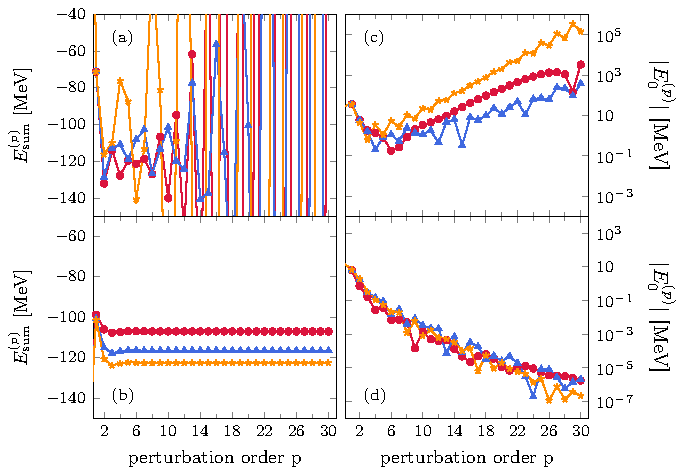
\includegraphics[width=0.8\textwidth]{thesis/doc/images/external/ho_vs_hf_mbpt.pdf}
  \caption[
    The partial sums (left) and order-by-order contributions (right)
    for an MBPT calculation of the ground-state energy of ${}^{16}\text{O}$
    using a harmonic-oscillator reference state (top)
    and a Hartree-Fock reference state (bottom).
    The red, blue, and yellow points are for $N_{\text{max}}=2$, 4, and 6,
    the basis truncation parameter for the approach used.
  ]{
    The partial sums (left) and order-by-order contributions (right)
    for an MBPT calculation of the ground-state energy of ${}^{16}\text{O}$
    using a harmonic-oscillator reference state (top)
    and a Hartree-Fock reference state (bottom).
    The red, blue, and yellow points are for $N_{\text{max}}=2$, 4, and 6,
    the basis truncation parameter for the approach used.
    Figure taken from Ref.~\cite{Tich16hohfmbpt}.
  }\label{fig:ho_vs_hf_mbpt}
\end{figure}

At the third order, even considering only canonical diagrams,
the number of diagrams possible with two- and three-body operators grows to 17.
The complete list of these diagrams can be found in Ref.~\cite{Hu18mbptthreebody}.
The canonical contributions involving only the normal-ordered two-body Hamiltonian are
\begin{equation}
  \begin{split}
    E^{(3)}_{\text{2-body only}} =
    &\frac{1}{8} \sum_{abcdij} \frac{\hnotwo_{ijab} \hnotwo_{abcd}\hnotwo_{cdij}}{\epsilon_{ij}^{ab}\epsilon_{ij}^{cd}} \\
    &+ \frac{1}{8} \sum_{abijkl} \frac{\hnotwo_{ijab} \hnotwo_{abkl}\hnotwo_{klij}}{\epsilon_{ij}^{ab}\epsilon_{kl}^{ab}} \\
    &- \sum_{abcijk} \frac{\hnotwo_{ijab} \hnotwo_{kbic}\hnotwo_{ackj}}{\epsilon_{ij}^{ab}\epsilon_{kj}^{ac}}\,.
  \end{split}
\end{equation}
The complete set of non-canonical third-order contributions
with only one- and two-body operators
is given, among other places, in Ref.~\cite{Tich17phd}.

The inclusion of additional terms is not the only challenge when dealing with a non-canonical reference state.
Choosing a different reference state than the HF determinant
corresponds to choosing a worse partitioning for $H$,
that is, more information is held in the perturbation $H_1$,
as the HF determinant is the best possible single Slater determinant approximation
to the ground state.
This less optimal choice can lead to poor convergence behavior of MBPT~\cite{Tich16hohfmbpt}.
For instance, in Fig.~\ref{fig:ho_vs_hf_mbpt}
the ground-state energy of ${}^{16}\text{O}$ was calculated
using a harmonic-oscillator determinant and a Hartree-Fock determinant
for the reference state.
While for the HF reference state MBPT converges nicely,
for the HO reference state the calculation rapidly begins to diverge
when going to higher orders in perturbation theory.
Additionally,
while MBPT benefits strongly from working with SRG-evolved Hamiltonians,
it can have difficulty converging even when using an HF reference state
for un-evolved nuclear Hamiltonians that are too ``hard''~\cite{Tich20mbptreview}.

\section{Non-perturbative techniques}

The convergence challenges of MBPT motivate us to consider non-perturbative many-body methods,
which sum to all orders certain types of diagrams to produce a convergent result.
Coupled cluster theory and the in-medium similarity renormalization group
are two examples of such methods.
Their non-perturbative nature makes them less sensitive to the choice of reference state
(although convergence speed will be affected by a non-canonical choice of reference state)
and better able to deal with ``harder'' nuclear Hamiltonians.
We discuss the IMSRG in detail in the next chapter.
Here, we aim to briefly introduce the coupled cluster many-body approach
as it shares many similarities with the IMSRG.\@

The ansatz for the coupled cluster (CC) approach is describing the ground state as
\begin{equation}
  \ket{\Psi} = \exp(T)\ket{\Phi}\,,
\end{equation}
where $T$ is the cluster operator,
which when applied exponentially to the reference state $\refgnd$ yields the ground state~\cite{Hage13ccreview}.
$T$ contains in general one- through $A$-body operators,
\begin{equation}
  T = \onebodyop{T} + \twobodyop{T} + \cdots + \abodyop{T}\,,
\end{equation}
which generate particle-hole excitations of the reference state.

The ground-state energy is then given by
\begin{align}
  E & = \braket{\Psi | H | \Psi}                                                           \\
    & = \braket{\Phi | \exp(-T) (\hnoone + \hnotwo + \hnothree) \exp(T) | \Phi} + \hnozero \\
    & \equiv \braket{\Phi | \overline{H} | \Phi} + \hnozero\,,
\end{align}
where we have defined the similarity-transformed Hamiltonian $\overline{H}$.
The task is to solve for matrix elements of the different $A$-body parts of $T$
such that
\begin{equation}
  0 = \braket{\Phi_{ijk\ldots}^{abc\ldots} | \overline{H} | \Phi}\,
\end{equation}
for all $n$-particle $n$-hole excited states of the reference state.
These are the coupled cluster equations.

One computes $\overline{H}$ via the Baker-Campbell-Hausdorff expansion,
\begin{equation}
  \overline{H} = H_N + \comm{H_N}{T} + \frac{1}{2!} \comm{\comm{H_N}{T}}{T} + \ldots \,,
\end{equation}
where $H_N \equiv \hnoone + \hnotwo + \hnothree$.
This commutator expansion ensures that only connected diagrams in the MBPT expansion are generated,
ensuring the size extensivity of the method.
A standard approach in nuclear physics is to truncate $T$, $H_N$, and the commutator
at the two-body level,
giving two coupled cluster equations
\begin{align}
  0 & = \braket{\Phi_{i}^{a} | \overline{H} | \Phi}\,,   \\
  0 & = \braket{\Phi_{ij}^{ab} | \overline{H} | \Phi}\,,
\end{align}
known as CCSD (SD for singles and doubles).
Another variant approximately treats the so-called triples and is denoted CCSD(T).\@
In the next chapter, when discussing the IMSRG,
the many similarities of the methods will be quite obvious.


\chapter{The in-medium similarity renormalization group}\label{ch:imsrg}

The in-medium similarity renormalization group
is a modern \abinitio{} many-body method
that extends the renormalization group approach of decoupling energy scales
to many-body calculations.
It is a non-perturbative many-body expansion method,
in the same vein as coupled cluster,
but it operates on the operators rather than the wave function.
It is remarkably flexible,
with favorable scaling with system size
and the ability to target many different observables,
and its invention and development has contributed strongly
to the rapid expansion of \abinitio{} theoretical calculations of medium-mass nuclei.
In this chapter, we introduce the IMSRG formalism.
We then discuss the topics of truncation scheme, generator selection,
and approaches to solving the flow equations.

\section{Basic formalism}

As a reminder from Section~\ref{sec:srg},
the idea behind the SRG is
the construction of a continuous unitary transformation of the Hamiltonian
\begin{equation}
  H(s) = U(s) H U^{\dagger}(s)\,,
\end{equation}
which can be obtained by solving the flow equation
\begin{equation}\label{eq:srg_flow_equation_imsrg}
  \frac{d H(s)}{ds} = [\eta(s), H(s)]\,,
\end{equation}
with the anti-Hermitian generator $\eta(s)$.
The solution of this flow equation with vacuum normal-ordered operators,
the free-space SRG,
is appealing in that the evolved operators are not system specific
and can be generally used for many-body calculations of nuclei and nuclear matter.
However, the free-space SRG evolution can only be done consistently
in the two- and three-body spaces for nuclear systems,
leaving out induced higher-body operators.

The idea behind the IMSRG is to solve Eq.~\eqref{eq:srg_flow_equation_imsrg} in-medium,
that is, to normal order with respect to a reference state before solving the flow equations.
Starting from a Hamiltonian with a one-, two- and three-body part
\begin{equation}
  H = \onebodyop{H} + \twobodyop{H} + \threebodyop{H}\,,
\end{equation}
our normal-ordered Hamiltonian matrix elements are given by
\begin{align}
  E             & \equiv \hnozero = \sum_i \onebodyop{H}_{ii} + \frac{1}{2}\sum_{ij} \twobodyop{H}_{ijij} + \frac{1}{6} \sum_{ijk} \threebodyop{H}_{ijkijk}\,, \\
  f_{pq}        & \equiv \hnoone_{pq} = \onebodyop{H}_{pq} + \sum_i \twobodyop{H}_{piqi} + \frac{1}{2} \sum_{ij} \threebodyop{H}_{pijqij} \,,                  \\
  \Gamma_{pqrs} & \equiv \hnotwo_{pqrs} = \twobodyop{H}_{pqrs} + \sum_i \threebodyop{H}_{pqirsi} \,,                                                           \\
  W_{pqrstu}    & \equiv \hnothree_{pqrstu} = \threebodyop{H}_{pqrstu} \,,
\end{align}
where we have introduced the conventional names
for zero-, one-, two-, and three-body normal-ordered parts of the Hamiltonian,
$E$, $f$, $\Gamma$, and $W$,
used in the literature.
As a reminder,
indices $p$, $q$, $r$, \ldots\ run over all single-particle states,
indices $i$, $j$, $k$, \ldots\ run over holes,
single-particle states occupied in the reference state,
and indices $a$, $b$, $c$, \ldots\ run over particles,
single-particle states unoccupied in the reference state.

In general, the generator $\eta(s)$ has one- through $A$-body normal-ordered parts
\begin{equation}
  \eta(s) = \sum_{i=1}^A \eta^{(i)}(s)\,.
\end{equation}
For now, we leave $\eta(s)$ unspecified beyond its required anti-Hermiticity,
which causes it to not have a zero-body part.
We discuss the choice of generator in Section~\ref{sec:imsrg_generator}.
Concretely, our initial normal-ordered Hamiltonian is
\begin{equation}
  \begin{split}
    H = &\,E
    + \sum_{pq} f_{pq} \noref{\crea{p} \annih{q}} \\
    &+ \frac{1}{{(2!)}^2} \sum_{pqrs} \Gamma_{pqrs} \noref{\crea{p} \crea{q} \annih{s} \annih{r}}\\
    &+ \frac{1}{{(3!)}^2} \sum_{pqrstu} W_{pqrstu} \noref{\crea{p} \crea{q} \crea{r} \annih{u} \annih{t} \annih{s}}\,,
  \end{split}
\end{equation}
and our generator is
\begin{equation}
  \begin{split}
    \eta(s) = &
    \sum_{pq} \eta^{(1)}_{pq}(s) \noref{\crea{p} \annih{q}} \\
    &+ \frac{1}{{(2!)}^2} \sum_{pqrs} \eta^{(2)}_{pqrs}(s) \noref{\crea{p} \crea{q} \annih{s} \annih{r}}\\
    &+ \frac{1}{{(3!)}^2} \sum_{pqrstu} \eta^{(3)}_{pqrstu}(s) \noref{\crea{p} \crea{q} \crea{r} \annih{u} \annih{t} \annih{s}}\\
    &+ \ldots \,.
  \end{split}
\end{equation}

The evaluation of the right-hand side of Eq.~\eqref{eq:srg_flow_equation_imsrg} then reduces to
the evaluation of commutators of normal-ordered products,
\begin{equation}
  \left[\noref{\crea{p_1} \ldots \crea{p_M} \annih{q_M} \ldots \annih{q_1}},
    \noref{\crea{r_1} \ldots \crea{r_N} \annih{s_N} \ldots \annih{s_1}}\right]\,,
\end{equation}
which can be simplified into a sum of normal-ordered operators
using the generalized Wick's theorem [see Eq.~\eqref{eq:gen_wicks_theorem}].
The commutator of a $K$-body operator $A^{(K)}$ and an $L$-body operator $B^{(L)}$
will in general have contributions of $|K-L|$-body operators through $K+L-1$-body operators,
\begin{equation}
  [A^{(K)}, B^{(L)}] = \sum_{M=|K-L|}^{K+L-1}C^{(M)}\,.
\end{equation}

The right-hand side can then be broken up into zero- through $A$-body parts.
We then identify the zero-body part of the right-hand side with $dE/ds$,
the one-body part with $df_{pq}/ds$, and so on.
This makes it obvious that
even if the initial Hamiltonian and generator contain only up to three-body operators
the IMSRG evolution induces higher-body operators,
all the way up to $A$-body operators after a couple integration steps,
resulting in coupled flow equations for the zero- through $A$-body parts
of the Hamiltonian.
Note that one must also ensure the antisymmetry of the right-hand sides of the two-,
three-, and higher-body flow equations
so the matrix elements remain antisymmetric.

The discussion here has been focused on the Hamiltonian,
but the IMSRG can also be used to evolve other operators,
\begin{equation}
  \frac{dO}{ds} = \comm{\eta(s)}{O(s)}\,,
\end{equation}
where $O$ has also been normal ordered with respect to our reference state $\refgnd$.
Since the generator $\eta(s)$ should be the same for the evolution of $H$ and $O$
and the reconstruction of the unitary transformation from the evolved form of $H$
is not possible,
$H$ and $O$ must naively be evolved simultaneously.
In Section~\ref{sec:imsrg_magnus}, we discuss an alternative approach to solving the IMSRG flow equations
that allows for the construction of the unitary transformation,
resulting in easy evolution of other operators along with the Hamiltonian.

\section{Truncation schemes}

As is the case with the free-space SRG,
it is not feasible to do the full $A$-body evolution,
and the flow equations must be truncated at some $B$-body level.
However, the situation is not quite the same as with the free-space SRG.\@
Because the initial normal ordering shifts information about higher-body operators
into lower-body normal-ordered operators
and the continuous normal ordering absorbs information about induced higher-body operators
into lower-body normal-ordered operators,
the truncated IMSRG flow equations still approximately evolve higher-body operators
(in the free-space sense)
using only the reduced $B$-body flow equations.
In the following sections,
we discuss truncating the IMSRG at the two-body and three-body level,
yielding the so-called IMSRG(2) and IMSRG(3) truncations respectively.

\subsection{IMSRG(2)}

Truncating the flow equation at the two-body level amounts to assuming
\begin{align}
  H(s)    & \approx E(s) + f(s) + \Gamma(s)\,,       \\
  \eta(s) & \approx \eta^{(1)}(s) + \eta^{(2)}(s)\,.
\end{align}
In this approximation,
we are not including the three-body part of the initial Hamiltonian exactly.
However, the three-body force \textit{does} contribute
as it was used in obtaining the normal-ordered zero-, one-, and two-body parts
of the Hamiltonian.
The only part that is being discarded is the residual three-body part, $W$.
This is known as the normal-ordered two-body (NO2B) approximation,
which has been quite successful in nuclear many-body applications.

Using the generalized Wick's theorem,
which yields the fundamental commutators in Appendix~\ref{app:mscheme_fundamental_commutators}
or also in Appendix A of Ref.~\cite{Herg15imsrgphysrep},
one arrives at the flow equations for the Hamiltonian
\begin{align}
  \phantom{\frac{d\Gamma_{ijkl}}{ds}}
   & \begin{aligned}
    \mathllap{\frac{dE}{ds}} & = \sum_{ab} n_{a} \bar{n}_{b}
    (\genone_{ab} f_{ba} - f_{ab} \genone_{ba})                                              \\
                             & \quad + \frac{1}{4} \sum_{abcd} n_{a}n_{b}\bar{n}_c \bar{n}_d
    (\gentwo_{abcd} \Gamma_{cdab} - \Gamma_{abcd}\gentwo_{cdab})\,,
  \end{aligned}\label{eq:imsrg2_0body} \\
   & \begin{aligned}
    \mathllap{\frac{df_{ij}}{ds}} & =
    \sum_{a}(\genone_{ia} f_{aj} - f_{ia} \genone_{aj})                                                          \\
                                  & \quad+\sum_{ab}(n_a - n_b)(\genone_{ab}\Gamma_{biaj} - f_{ab}\gentwo_{biaj}) \\
                                  & \quad+\frac{1}{2}\sum_{abc}(\bar{n}_a \bar{n}_b n_c + n_a n_b \bar{n}_c)
    (\gentwo_{ciab} \Gamma_{abcj} - \Gamma_{ciab} \gentwo_{abcj})\,,
  \end{aligned}\label{eq:imsrg2_1body} \\
   & \begin{aligned}
    \mathllap{\frac{d\Gamma_{ijkl}}{ds}} & =
    \sum_{a}(1 - P_{ij})(\genone_{ia}\Gamma_{ajkl} - f_{ia}\gentwo_{ajkl})                                                                            \\
                                         & \quad - \sum_{a}(1 - P_{kl})(\genone_{ak}\Gamma_{ijal} - f_{ak}\gentwo_{ijal})                             \\
                                         & \quad + \frac{1}{2}\sum_{ab}(1 - n_{a} - n_{b})(\gentwo_{ijab}\Gamma_{abkl} - \Gamma_{ijab}\gentwo_{abkl}) \\
                                         & \quad + \sum_{ab} (n_a - n_b)(1 - P_{ij})(1 - P_{kl})\gentwo_{aibk}\Gamma_{bjal}\,,
  \end{aligned}\label{eq:imsrg2_2body}
\end{align}
where $n_p$ are the occupation numbers of the reference state,
$\bar{n}_p \equiv 1 - n_p$,
the $s$-dependence has been suppressed,
and the permutation operator $P_{pq}$ exchanges the indices $p$ and $q$
in the following expression.
We have broken our usual notation for single-particle index labels
to adopt the following convention for the IMSRG flow equations:
the indices $i$,~$j$,~\ldots\ are for external indices
(indices on the flowing Hamiltonian),
and the indices $a$,~$b$,~\ldots\ are for contracted indices,
which are summed over in the flow equation.

Eqs.~\eqref{eq:imsrg2_0body}-\eqref{eq:imsrg2_2body} are solved by integrating
from $s=0$ towards $s\rightarrow\infty$ with the initial conditions
$E(0) = E$, $f(0) = f$, and $\Gamma(0)=\Gamma$.
Given appropriate decoupling (see Section~\ref{sec:imsrg_generator}),
$E(\infty)$ gives the energy of the state targeted by the reference state,
for our applications typically the ground state.
The cost of this integration is dominated by the final two terms in Eq.~\eqref{eq:imsrg2_2body},
which scale like $\mathcal{O}(N^6)$,
where $N$ is the size of the single-particle basis for the calculation.
Another nice property is that the flow equation,
due to being a commutator many-body expansion,
generates only connected diagrams and thus ensures size extensivity~\cite{Herg15imsrgphysrep}.
This is true for any $B$-body truncation.

\subsection{IMSRG(3)}\label{sec:imsrgthree}

Truncating at the three-body level allows one to exactly include initial three-body forces.
One assumes
\begin{align}
  H(s)    & \approx E(s) + f(s) + \Gamma(s) + W(s)\,,         \\
  \eta(s) & \approx \genone(s) + \gentwo(s) + \genthree(s)\,,
\end{align}
yielding additional terms with commutators of $\genthree$ and $W$
with zero- through two-body operators
and a commutator between $\genthree$ and $W$.
The flow equations are
\begin{align}
  \phantom{\frac{dW_{ijklmn}}{ds}}
   & \begin{aligned}
    \mathllap{\frac{dE}{ds}} & = \sum_{ab} n_{a} \bar{n}_{b}
    (\genone_{ab} f_{ba} - f_{ab} \genone_{ba})                                                            \\
                             & \quad + \frac{1}{4} \sum_{abcd} n_{a}n_{b}\bar{n}_c \bar{n}_d
    (\gentwo_{abcd} \Gamma_{cdab} - \Gamma_{abcd}\gentwo_{cdab})                                           \\
                             & \quad + \frac{1}{36}\sum_{abcdef} n_a n_b n_c \bar{n}_d \bar{n}_e \bar{n}_f
    (\genthree_{abcdef} W_{defabc} - W_{abcdef} \genthree_{defabc})\,,
  \end{aligned}\label{eq:imsrg3_0body} \\
   & \begin{aligned}
    \mathllap{\frac{df_{ij}}{ds}} & =
    \sum_{a}(\genone_{ia} f_{aj} - f_{ia} \genone_{aj})                                                                       \\
                                  & \quad+\sum_{ab}(n_a - n_b)(\genone_{ab}\Gamma_{biaj} - f_{ab}\gentwo_{biaj})              \\
                                  & \quad+\frac{1}{2}\sum_{abc}(\bar{n}_a \bar{n}_b n_c + n_a n_b \bar{n}_c)
    (\gentwo_{ciab} \Gamma_{abcj} - \Gamma_{ciab} \gentwo_{abcj})                                                             \\
                                  & \quad - \frac{1}{4} \sum_{abcd}(n_a n_b \bar{n}_c \bar{n}_d -\bar{n}_a \bar{n}_b n_c n_d)
    (\gentwo_{cdab} W_{abijcd} - \Gamma_{cdab} \genthree_{abijcd})                                                            \\
                                  & \quad + \frac{1}{12}\sum_{abcde}
    (n_a n_b \bar{n}_c \bar{n}_d \bar{n}_e + \bar{n}_a \bar{n}_b n_c n_d n_e)
    (\genthree_{abicde} W_{cdeabj} - W_{abicde} \genthree_{cdeabj})\,,
  \end{aligned}\label{eq:imsrg3_1body} \\
   & \begin{aligned}
    \mathllap{\frac{d\Gamma_{ijkl}}{ds}} & =
    \sum_{a}(1 - P_{ij})(\genone_{ia}\Gamma_{ajkl} - f_{ia}\gentwo_{ajkl})                                                                            \\
                                         & \quad - \sum_{a}(1 - P_{kl})(\genone_{ak}\Gamma_{ijal} - f_{ak}\gentwo_{ijal})                             \\
                                         & \quad + \frac{1}{2}\sum_{ab}(1 - n_{a} - n_{b})(\gentwo_{ijab}\Gamma_{abkl} - \Gamma_{ijab}\gentwo_{abkl}) \\
                                         & \quad + \sum_{ab} (n_a - n_b)(1 - P_{ij})(1 - P_{kl})\gentwo_{aibk}\Gamma_{bjal}                           \\
                                         & \quad + \sum_{ab} (n_a - n_b)(\genone_{ab} W_{bijakl} - f_{ab} \genthree_{bijakl})                         \\
                                         & \quad - \frac{1}{2} \sum_{abc} (n_a \bar{n}_b \bar{n}_c + \bar{n}_a n_b n_c)
    (1 - P_{kl})(\gentwo_{bcak} W_{aijbcl} - \Gamma_{bcak} \genthree_{aijbcl})                                                                        \\
                                         & \quad + \frac{1}{2} \sum_{abc} (n_a \bar{n}_b \bar{n}_c + \bar{n}_a n_b n_c)
    (1 - P_{ij})(\gentwo_{bcai} W_{aklbcj} - \Gamma_{bcai} \genthree_{aklbcj})                                                                        \\
                                         & \quad + \frac{1}{6} \sum_{abcd}(n_a \bar{n}_b \bar{n}_c \bar{n}_d -\bar{n}_a n_b n_c n_d)
    (\genthree_{aijbcd} W_{bcdakl} - W_{aijbcd} \genthree_{bcdakl})                                                                                   \\
                                         & \quad + \frac{1}{4} \sum_{abcd}(\bar{n}_a \bar{n}_b n_c n_d -n_a n_b \bar{n}_c \bar{n}_d)
    (1 - P_{ij})(1 - P_{kl}) \genthree_{abicdl} W_{cdjabk}\,,
  \end{aligned}\label{eq:imsrg3_2body} \\
   & \begin{aligned}
    \mathllap{\frac{dW_{ijklmn}}{ds}} & =
    \sum_{a} P(i/jk) (\genone_{ia} W_{ajklmn} - f_{ia} \genthree_{ajklmn})                                                     \\
                                      & \quad - \sum_{a} P(l/mn) (\genone_{al} W_{ijkamn} - f_{al} \genthree_{ijkamn})         \\
                                      & \quad + \sum_{a} P(ij/k) P(l/mn)
    (\gentwo_{ijla} \Gamma_{akmn} - \Gamma_{ijla} \gentwo_{akmn})                                                              \\
                                      & \quad + \frac{1}{2} \sum_{ab} (1 - n_a - n_b) P(ij/k)
    (\gentwo_{ijab} W_{abklmn} - \Gamma_{ijab} \genthree_{abklmn})                                                             \\
                                      & \quad - \frac{1}{2} \sum_{ab} (1 - n_a - n_b) P(l/mn)
    (\gentwo_{abmn} W_{ijklab} - \Gamma_{abmn} \genthree_{ijklab})                                                             \\
                                      & \quad + \frac{1}{6} \sum_{abc} (n_a n_b n_c + \bar{n}_a \bar{n}_b \bar{n}_c)
    (\genthree_{ijkabc} W_{abclmn} - W_{ijkabc} \genthree_{abclmn})                                                            \\
                                      & \quad + \frac{1}{2} \sum_{abc} (n_a n_b \bar{n}_c + \bar{n}_a \bar{n}_b n_c)
    P(ij/k)P(l/mn)                                                                                                             \\
                                      & \qquad \qquad \times (\genthree_{abkcmn} W_{cijabl} -\genthree_{cjkabn} W_{iablmc})\,,
  \end{aligned}\label{eq:imsrg3_3body}
\end{align}
Here, $P(pq/r) = 1 - P_{pr} - P_{qr}$ and $P(p/qr) = 1 - P_{pq} - P_{pr}$
ensure the antisymmetry of the three-body indices.

It is clear that the final two terms in Eq.~\eqref{eq:imsrg3_3body}
dominate the cost of the integration,
scaling like $\mathcal{O}(N^9)$ in the size of our single-particle basis.
In the absence of an initial three-body operator,
the third term in Eq.~\eqref{eq:imsrg3_3body},
the three-body part of the commutator of two two-body operators,
induces a three-body operator,
which leads to the contribution of all other terms later in the integration.

We would also like to note that
in the derivation of the flow equations here
the only assumption that was made was that
two- and three-body matrix elements are appropriately antisymmetric.
In particular, unlike several other references in the literature,
for instance Refs.~\cite{Herg15imsrgphysrep,Tsuk10imsrg},
the flow equations here do not assume $f$, $\Gamma$, and $W$ are Hermitian
(which of course they are).
While this assumption allows for the simplification of certain terms
(nothing that changes the scaling of the terms however),
it limits the expressions to only commutators of anti-Hermitian and Hermitian operators.
In Section~\ref{sec:imsrg_magnus},
we require the commutator of two anti-Hermitian operators,
for which the right-hand sides of
Eqs.~\eqref{eq:imsrg2_0body}-\eqref{eq:imsrg2_2body}
and Eqs.~\eqref{eq:imsrg3_0body}-\eqref{eq:imsrg3_3body}
are equally valid.
For numerical implementations,
it is a good idea to implement each of the fundamental commutators separately,
to allow for validation and fine-grained optimization in the most expensive commutators.

\section{Generator selection}\label{sec:imsrg_generator}

\begin{figure}[t]
  \setlength{\unitlength}{0.8\columnwidth}
  \begin{center}
    \begin{picture}(1.0000,0.5500)
      \put(0.0350,0.0450){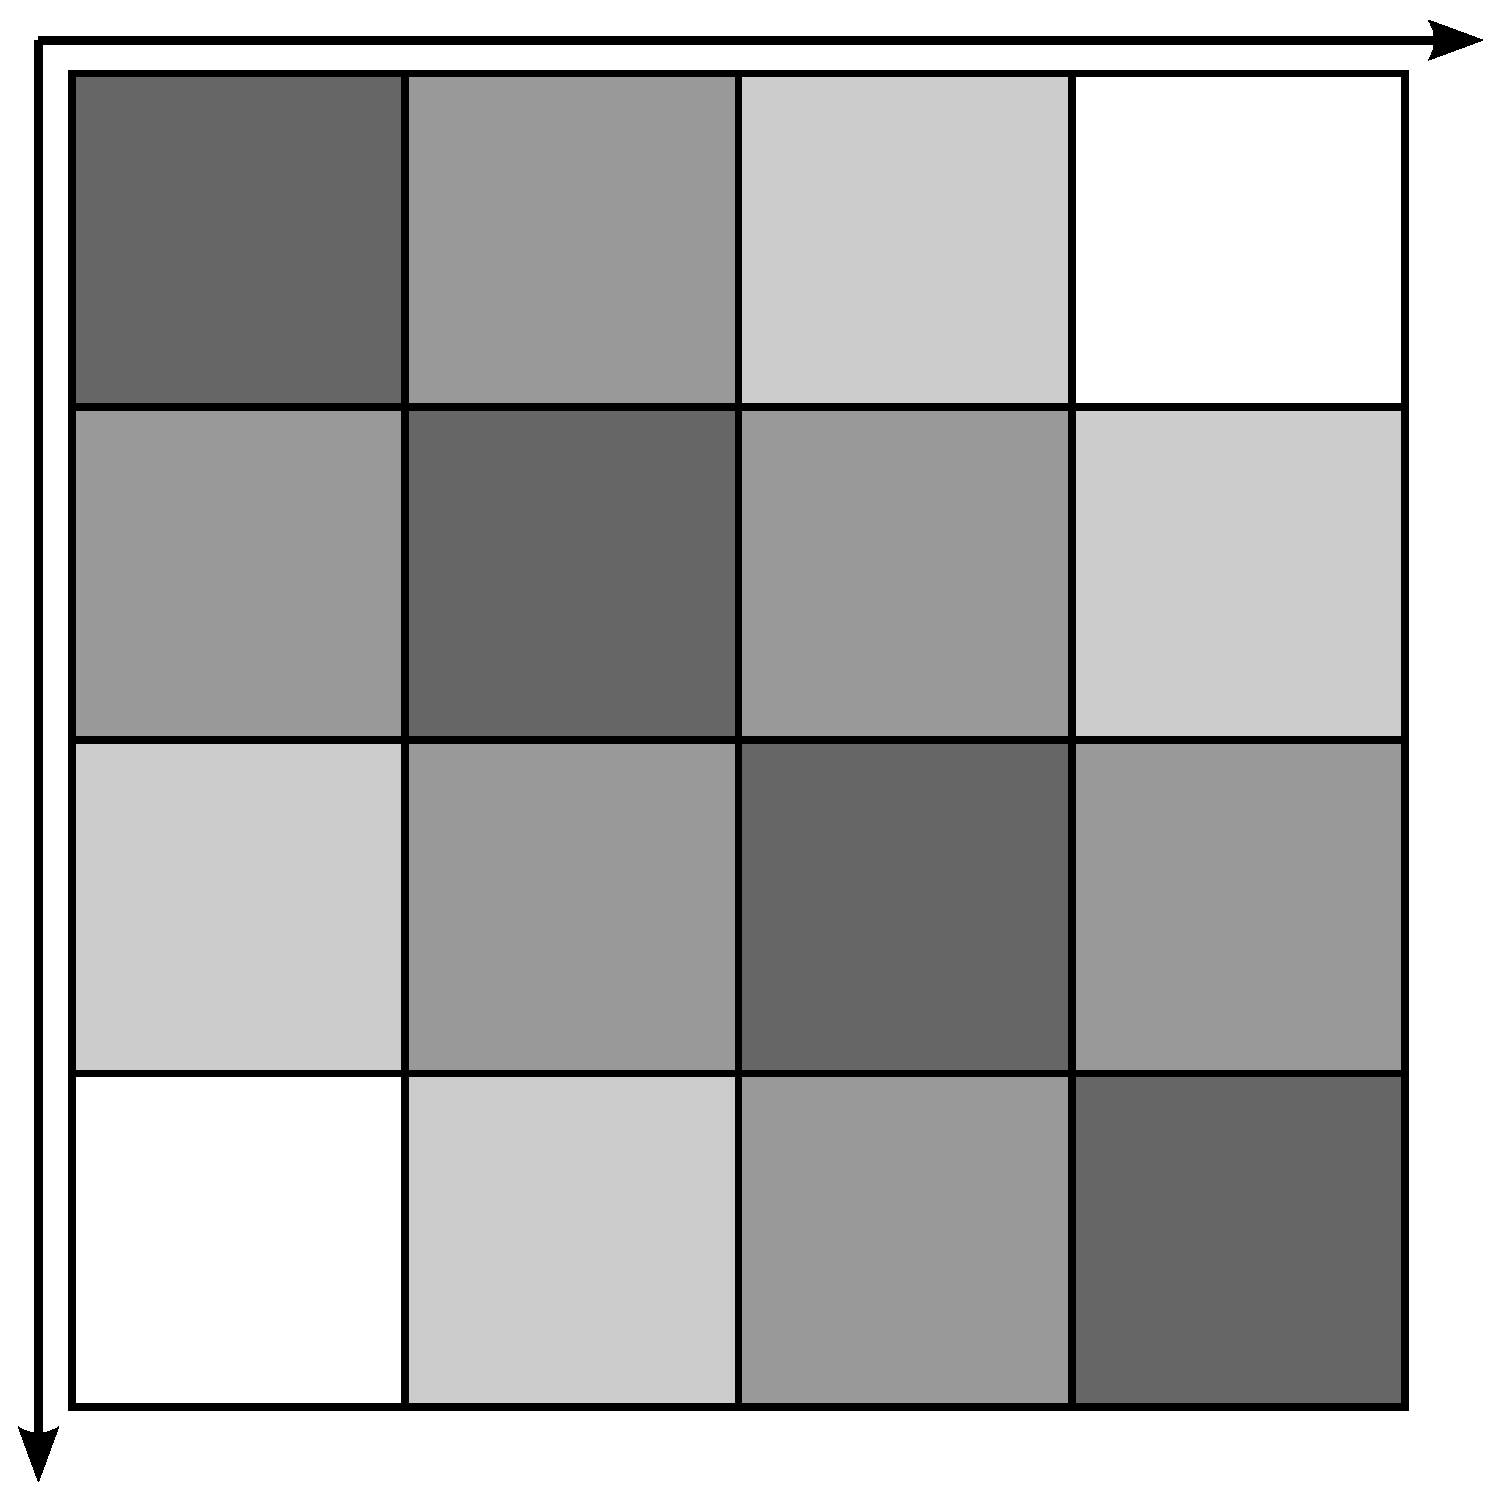
\includegraphics[width=0.46\unitlength]{thesis/doc/images/external/H_initial.eps}}
      \put(0.5400,0.0450){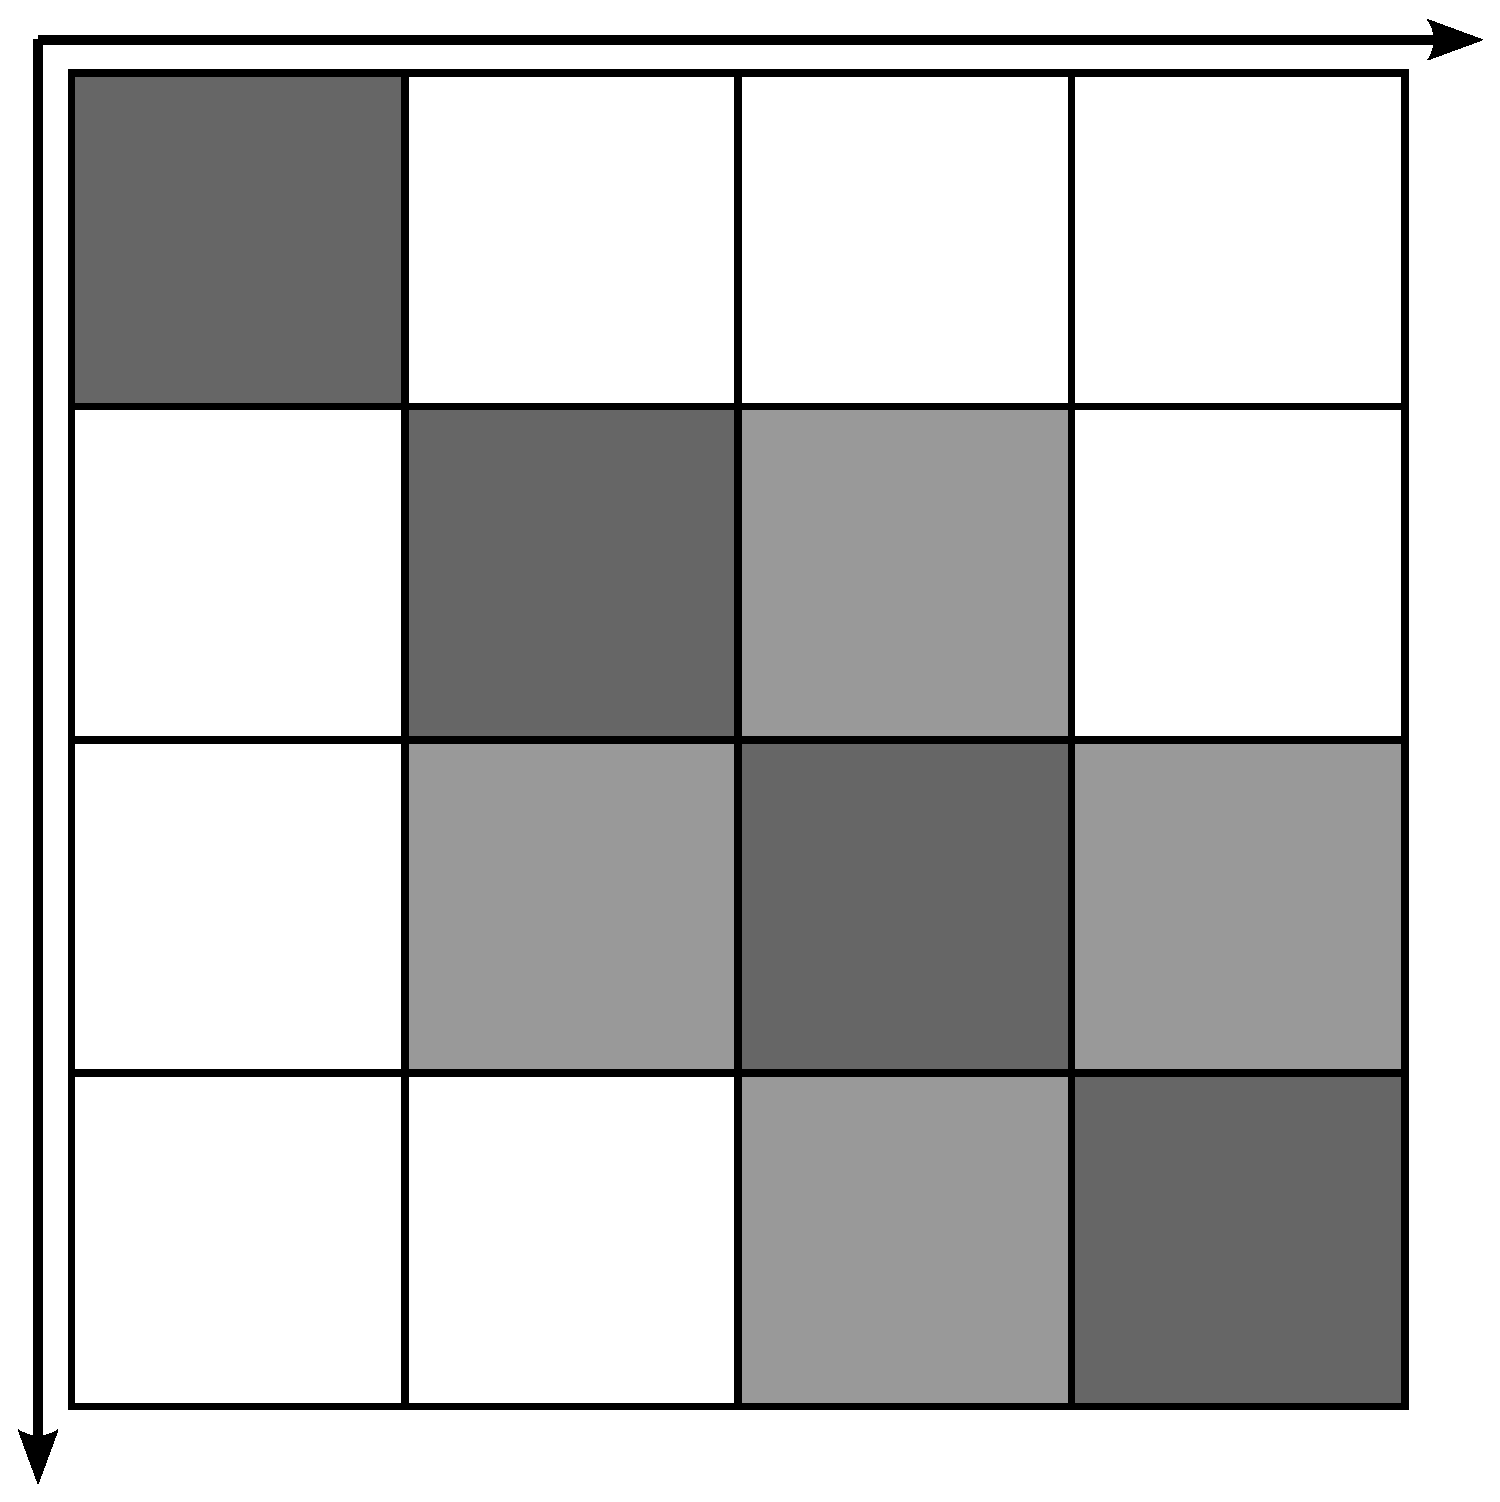
\includegraphics[width=0.46\unitlength]{thesis/doc/images/external/H_IMSRG_3ph_decoupling.eps}}
      \put(0.0100,0.0000){\parbox{0.5\unitlength}{\centering$\braket{i|H(0)|j}$}}
      \put(0.5200,0.0000){\parbox{0.5\unitlength}{\centering$\braket{i|H(\infty)|j}$}}

      \put(0.0500,0.5100){\parbox{0.11\unitlength}{\centering\footnotesize0p0h}}
      \put(0.1600,0.5100){\parbox{0.11\unitlength}{\centering\footnotesize1p1h}}
      \put(0.2630,0.5100){\parbox{0.11\unitlength}{\centering\footnotesize2p2h}}
      \put(0.3650,0.5100){\parbox{0.11\unitlength}{\centering\footnotesize3p3h}}
      \put(0.5500,0.5100){\parbox{0.11\unitlength}{\centering\footnotesize0p0h}}
      \put(0.6600,0.5100){\parbox{0.11\unitlength}{\centering\footnotesize1p1h}}
      \put(0.7630,0.5100){\parbox{0.11\unitlength}{\centering\footnotesize2p2h}}
      \put(0.8650,0.5100){\parbox{0.11\unitlength}{\centering\footnotesize3p3h}}
      %
      \put(0.0100,0.4320){\parbox{0.11\unitlength}{\rotatebox{90}{\centering\footnotesize0p0h}}}
      \put(0.0100,0.3235){\parbox{0.11\unitlength}{\rotatebox{90}{\centering\footnotesize1p1h}}}
      \put(0.0100,0.2175){\parbox{0.11\unitlength}{\rotatebox{90}{\centering\footnotesize2p2h}}}
      \put(0.0100,0.1100){\parbox{0.11\unitlength}{\rotatebox{90}{\centering\footnotesize3p3h}}}

      \put(0.5100,0.4320){\parbox{0.11\unitlength}{\rotatebox{90}{\centering\footnotesize0p0h}}}
      \put(0.5100,0.3235){\parbox{0.11\unitlength}{\rotatebox{90}{\centering\footnotesize1p1h}}}
      \put(0.5100,0.2175){\parbox{0.11\unitlength}{\rotatebox{90}{\centering\footnotesize2p2h}}}
      \put(0.5100,0.1100){\parbox{0.11\unitlength}{\rotatebox{90}{\centering\footnotesize3p3h}}}
    \end{picture}
  \end{center}
  \caption[
    Schematic diagram
    showing the minimal decoupling scheme
    taken in the IMSRG.\@
  ]{\label{fig:imsrg_decoupling}
    Schematic diagram
    showing the minimal decoupling scheme
    taken in the IMSRG.\@
    Figure taken from Ref.~\cite{Herg15imsrgphysrep}.
  }
\end{figure}

So far, we have not discussed specific choices of our generator $\eta$.
The possible definitions of $\eta$ hinge on the specification
of our so-called ``off-diagonal'' Hamiltonian $H_{od}$,
the part of the Hamiltonian we wish to suppress
to ensure appropriate decoupling in the remaining ``diagonal'' part.
In Section~\ref{sec:srg},
we saw that the generator choice
$\eta(s) = \comm{T_{\text{rel}}}{H(s)}$
leads to the decoupling of any two states
with a decay scale set by the difference in their kinetic energy expectation values.
The result is that the Hamiltonian evolves towards a diagonal form,
providing vastly improved convergence
and allowing many-body calculations to use significantly smaller model spaces.

To identify the desired decoupling for the IMSRG,
we begin by considering the Hamiltonian in the basis spanned by
our reference state $\refgnd$ and
$n$-particle $n$-hole ($npnh$) excitations of the reference state,
\begin{equation}
  \{\refgnd, \refhp{i}{a}, \refhp{ij}{ab}, \refhp{ijk}{abc}, \ldots \}\,.
\end{equation}
For a Hamiltonian with only one- and two-body operators,
as is the approximation after normal ordering for the IMSRG(2) truncation,
the Hamiltonian in this basis is schematically represented
in the left panel of Fig.~\ref{fig:imsrg_decoupling}.
It is band-diagonal and only able to couple an $npnh$ excitation
to $(n\pm2)p(n\pm2)h$ excitations.
For a Hamiltonian with a three-body part,
the band diagonal grows to include $(n\pm3)p(n\pm3)h$ excitations.

For the IMSRG,
a decoupling towards a true diagonal form is no longer a good idea,
as one must avoid inducing significant three-body terms in the IMSRG(2)
or four- and higher-body terms in the IMSRG(3)
to maintain the validity of the truncation.
The alternative is a minimal decoupling scheme,
where the sole objective is to decouple the reference state $\refgnd$
from all $npnh$ excitations,
as shown in the right panel of Fig.~\ref{fig:imsrg_decoupling}.
Achieving this decoupling gives us the energy of the state $E$
in the zero-body part of the normal-ordered Hamiltonian
and the corresponding eigenstate by applying the unitary transformation
to the reference state, $U^{\dagger}(\infty)\refgnd$.
For some finite truncation of the flow equations,
this result is of course only approximate.

Now that we know we want to suppress the matrix elements
that couple $\refgnd$ to its excitations,
we want to identify which parts of our normal-ordered Hamiltonian
these matrix elements correspond to.
For the couplings between $\refgnd$ and $1p1h$ excitations, we find
\begin{align}
  \phantom{\braket{\Phi | H |\Phi_{i}^{a}}}
   & \begin{aligned}
    \mathllap{\braket{\Phi | H |\Phi_{i}^{a}}} & = \braket{\Phi | H \noref{\crea{a} \annih{i}}| \Phi}
  \end{aligned} \\
   & \begin{aligned}
    \mathllap{} & = E \braket{\Phi | \noref{\crea{a} \annih{i}} | \Phi}                                               \\
                & \quad + \sum_{pq} f_{pq} \braket{\Phi |\noref{\crea{p}\annih{q}} \noref{\crea{a} \annih{i}} | \Phi} \\
                & \quad + \sum_{pqrs} \Gamma_{pqrs}
    \braket{\Phi |\noref{\crea{p} \crea{q} \annih{s} \annih{r}}\noref{\crea{a} \annih{i}} | \Phi}
  \end{aligned} \\
   & \begin{aligned}
    \mathllap{} & = \sum_{pq} f_{pq} \delta_{pi} \delta_{qa} n_{i} \bar{n}_{a}
  \end{aligned} \\
   & \begin{aligned}
    \mathllap{} & = f_{ia}\,.
  \end{aligned}
\end{align}
Via similar calculations, one finds
\begin{samepage}
  \begin{subequations}
    \begin{align}
      \begin{split}
        \braket{\Phi_{i}^{a} | H | \Phi} &= f_{ai}\,,
      \end{split} \\
      \begin{split}
        \braket{\Phi | H | \Phi_{ij}^{ab}} &= \Gamma_{ijab}\,,
      \end{split} \\
      \begin{split}
        \braket{\Phi_{ij}^{ab} | H | \Phi} &= \Gamma_{abij}\,,
      \end{split} \\
      \begin{split}
        \braket{\Phi | H | \Phi_{ijk}^{abc}} &= W_{ijkabc}\,,
      \end{split} \\
      \begin{split}
        \braket{\Phi_{ijk}^{abc} | H | \Phi} &= W_{abcijk}\,.
      \end{split}
    \end{align}
  \end{subequations}
\end{samepage}
We define our ``off-diagonal'' normal-ordered Hamiltonian then to be
\begin{equation}
  \begin{split}
    H_{od} \equiv & \sum_{ia}\left(f_{ia} \noref{\crea{i}\annih{a}}
    + f_{ai} \noref{\crea{a}\annih{i}}\right) \\
    & + \frac{1}{{(2!)}^2}\sum_{ijab} \left(
    \Gamma_{ijab} \noref{\crea{i}\crea{j}\annih{b}\annih{a}}
    + \Gamma_{abij} \noref{\crea{a}\crea{b}\annih{j}\annih{i}}
    \right) \\
    & + \frac{1}{{(3!)}^2}\sum_{ijkabc} \left(
    W_{ijkabc} \noref{\crea{i}\crea{j}\crea{k}\annih{c}\annih{b}\annih{a}}
    + W_{abcijk} \noref{\crea{a}\crea{b}\crea{c}\annih{k}\annih{j}\annih{i}}
    \right)\,.
  \end{split}
\end{equation}
We are now in a position where we can define generators that suppress these matrix elements
over the course of the flow.

Wegner's original ansatz for the generator of the SRG flow equation is
\begin{equation}
  \eta(s) = \comm{H_d(s)}{H_{od}(s)}\,,
\end{equation}
where $H_d = H - H_{od}$~\cite{Wegn94srg}.
When using $H_{od}$ as defined above,
one can evaluate the commutator truncating at the two- or three-body level
depending on the truncation scheme,
giving the one-, two-, and three-body components of $\eta$
in the same form as Eqs.~\eqref{eq:imsrg3_0body}-\eqref{eq:imsrg3_3body}.
A perturbative analysis of the flow equations with this choice of generator,
as is done in Ref.~\cite{Herg16imsrglecnotes},
reveals that the two-body ``off-diagonal'' matrix elements are suppressed like
\begin{equation}
  \Gamma_{abij}(s) \approx \Gamma_{abij}(0) \exp(-{(\Delta_{abij})}^{2} s)\,,
\end{equation}
where $\Delta_{abij}$ are the energy denominators.
There are multiple options for these energy denominators,
corresponding to different partitionings in MBPT (see Section~\ref{sec:mbpt}).
We choose to focus on the M{\o}ller-Plesset denominators,
with $\Delta_{abij} = \epsilon_{abij}$ from Eq.~\eqref{eq:mp_energy_denom}.
Another alternative is the Epstein-Nesbet denominators
(see Ref.~\cite{Shav09mbpt_cc_book} for details).

We have included the Wegner generator in this discussion for completeness
but will not use it in any applications.
One reason for this is that the Wegner generator is simply more expensive to construct
than the alternatives,
which give explicit expressions for the matrix elements of $\eta$,
resulting in scaling of $\mathcal{O}(N^4)$ and $\mathcal{O}(N^6)$ for IMSRG(2) and IMSRG(3),
respectively.
This is to be contrasted with the evaluation of a full commutator,
which scales like $\mathcal{O}(N^6)$ and $\mathcal{O}(N^9)$ for IMSRG(2) and IMSRG(3).
Additionally, the Wegner generator causes the system of differential equations
to be much more stiff,
making the integration much more expensive
(in terms of storage and computational requirements)
than for other generators.

The following generators directly construct the matrix elements of $\eta$, working with a basic form of
\begin{equation}
  \begin{split}
    \eta \equiv & \sum_{ia}\left(\genone_{ia} \noref{\crea{i}\annih{a}}
    + \genone_{ai} \noref{\crea{a}\annih{i}}\right) \\
    & + \frac{1}{{(2!)}^2} \sum_{ijab} \left(
    \gentwo_{ijab} \noref{\crea{i}\crea{j}\annih{b}\annih{a}}
    + \gentwo_{abij} \noref{\crea{a}\crea{b}\annih{j}\annih{i}}
    \right) \\
    & + \frac{1}{{(3!)}^2} \sum_{ijkabc} \left(
    \genthree_{ijkabc} \noref{\crea{i}\crea{j}\crea{k}\annih{c}\annih{b}\annih{a}}
    + \genthree_{abcijk} \noref{\crea{a}\crea{b}\crea{c}\annih{k}\annih{j}\annih{i}}
    \right)\,,
  \end{split}
\end{equation}
where we note that for $\eta$ to be anti-Hermitian, the matrix elements must fulfill
\begin{subequations}
  \begin{align}
    \begin{split}
      \genone_{ia} &= - \genone_{ai}\,,
    \end{split} \\
    \begin{split}
      \gentwo_{ijab} &= - \gentwo_{abij}\,,
    \end{split} \\
    \begin{split}
      \genthree_{ijkabc} &= - \genthree_{abcijk}\,.
    \end{split}
  \end{align}
\end{subequations}
The White generator corresponds to the choice
\begin{align}
  \genone_{ia}(s)       & = \frac{f_{ia}(s)}{\Delta_{ia}(s)}\,,          \\
  \gentwo_{ijab}(s)     & = \frac{\Gamma_{ijab}(s)}{\Delta_{ijab}(s)}\,, \\
  \genthree_{ijkabc}(s) & = \frac{W_{ijkabc}(s)}{\Delta_{ijkabc}(s)}\,,
\end{align}
where the antisymmetry of the denominators automatically gives the desired anti-Hermiticity~\cite{Whit02generator}.
The White generator suppresses off-diagonal matrix elements like
\begin{equation}
  \Gamma_{abij}(s) \approx \Gamma_{abij}(0) \exp(-s)\,,
\end{equation}
that is, it suppresses all off-diagonal matrix elements with the same decay scale,
regardless of the energy differences between the states.
This is unusual and not strictly speaking in line with the renormalization group approach,
where large energy-difference modes are integrated out first.
However, we are interested in $H(\infty)$ and $E(\infty)$,
and in this limit all generators that suppress $H_{od}$ produce identical results
for $E(\infty)$ and $U^{\dagger}(\infty)\refgnd$,
up to truncation effects.

A potential difficulty with the White generator arises
when one of the energy denominators becomes very small,
leading to large matrix elements of $\eta$
and thus extremely large derivatives in the right-hand side of the flow equation.
This can be mitigated by a variation of the standard White generator,
the arctan generator,
with generator matrix elements defined as
\begin{align}
  \genone_{ia}(s)       & = \frac{1}{2}\text{arctan}\left(\frac{2f_{ia}(s)}{\Delta_{ia}(s)}\right)\,,          \\
  \gentwo_{ijab}(s)     & = \frac{1}{2}\text{arctan}\left(\frac{2\Gamma_{ijab}(s)}{\Delta_{ijab}(s)}\right)\,, \\
  \genthree_{ijkabc}(s) & = \frac{1}{2}\text{arctan}\left(\frac{2W_{ijkabc}(s)}{\Delta_{ijkabc}(s)}\right)\,,
\end{align}
where the arctan function regularizes any possible large matrix elements that arise due to small energy denominators.

The final generator we discuss here is the imaginary-time generator,
which was ostensibly inspired by imaginary-time evolution techniques
in Quantum Monte Carlo methods~\cite{Herg15imsrgphysrep}.
Its matrix elements are defined as
\begin{align}
  \genone_{ia}(s)       & = \text{sign}(\Delta_{ia}(s))f_{ia}(s)\,,          \\
  \gentwo_{ijab}(s)     & = \text{sign}(\Delta_{ijab}(s))\Gamma_{ijab}(s)\,, \\
  \genthree_{ijkabc}(s) & = \text{sign}(\Delta_{ijkabc}(s))W_{ijkabc}(s)\,.
\end{align}
A perturbative analysis of the flow equations with this generator choice shows
that off-diagonal matrix elements are suppressed like
\begin{equation}
  \Gamma_{abij}(s) \approx \Gamma_{abij}(0) \exp(-|\Delta_{abij}|s)\,.
\end{equation}
The sign function in the definition of the generator ensures that
there is an absolute value around the energy denominator in the exponential,
giving a suppression for all matrix elements instead of an enhancement for some.
We also note here that the imaginary-time generator produces a ``proper'' RG flow,
where matrix elements coupling large energy differences are suppressed
before those coupling smaller energy differences.

\section{The Magnus expansion}\label{sec:imsrg_magnus}

Working with Eqs.~\eqref{eq:imsrg2_0body}-\eqref{eq:imsrg2_2body}
and~\eqref{eq:imsrg3_0body}-\eqref{eq:imsrg3_3body},
one can solve the IMSRG by numerically integrating
the system of ordinary differential equations (ODEs)
to obtain the energy and the expectation values of other observables in the targeted state.
This approach has two main challenges:
First, the flow equations need to be solved to high precision,
as otherwise numerical effects destroy the unitarity of the transformation
even in the absence of any truncation.
This necessitates the application of sophisticated ODE solvers
to minimize this numerical error.
These solvers require the allocation of several times the memory requirement
of two- and three-body operators,
which is already quite a lot (on the order of GB or tens of GB),
and the evaluation of each integration step is substantially more expensive
(providing the benefit of reduced accumulated numerical error)
than an Euler method.
This is incidentally also a reason the White, arctan, and imaginary-time generators
are preferred over the Wegner generator,
as the stiffness of the flow equations with the Wegner generator
requires the use of stiff ODE solvers,
which are even more expensive in terms of storage and computational cost
than their non-stiff counterparts.

Second, the evolution of other operators along with the Hamiltonian
requires them to be evolved in parallel in this approach.
This means that for every additional operator the memory and computational cost
increases by the amount that it would cost to just solve the Hamiltonian.
Furthermore, additional operators may increase the stiffness of the system of ODEs
as the integration scales for their matrix elements may differ from the Hamiltonian.
This challenge can be alleviated by the ability to construct the unitary transformation
for the evolution, $U(s)$.

This is the goal of the Magnus expansion approach to solving the IMSRG flow equations~\cite{Morr15magnus}.
Given our definition of $\eta(s)$ following Eq.~\eqref{eq:srg_flow_eq},
we get a differential equation for $U(s)$,
\begin{equation}
  \frac{dU(s)}{ds} = - \eta(s) U(s)\,,
\end{equation}
where $U(0) = 1$.
The formal integral of this differential equation is
\begin{equation}
  U(s) = \mathcal{T}_s\left[\exp(-\int_{0}^{s} ds' \eta(s'))\right]\,,
\end{equation}
where $\mathcal{T}_s$ is the time-ordering operator with respect to $s$~\cite{Dyso49timeorder}.

The Magnus expansion postulates that a solution of the form
\begin{equation}
  U(s) = \exp(\Omega(s))
\end{equation}
exists, where $\Omega(s)$ is anti-Hermitian and $\Omega(0) = 0$~\cite{Magn54magnus}.
To obtain $\Omega(s)$, one solves the differential equation of its expansion in $\eta(s)$,
\begin{equation}\label{eq:magnus_expansion}
  \frac{d \Omega(s)}{ds} = \sum_{k=0}^{\infty} \frac{B_{k}}{k!} ad^{k}_{\Omega(s)}(\eta(s))\,,
\end{equation}
where $B_{k}$ are the Bernoulli numbers
and $ad^{k}_{\Omega}$ are the recursively defined commutators,
\begin{align}
  ad^{0}_{\Omega(s)}(\eta(s)) & = \eta(s)\,,                                         \\
  ad^{k}_{\Omega(s)}(\eta(s)) & = \comm{\Omega(s)}{ad^{k-1}_{\Omega(s)}(\eta(s))}\,.
\end{align}
The interested reader may refer to Ref.~\cite{Blan09magnusreview} for detailed review
of the Magnus expansion.

Here we note that $ad^{k}_{\Omega(s)}(\eta(s))$ is anti-Hermitian for all $k$,
thus truncating Eq.~\eqref{eq:magnus_expansion} at any order
gives an exactly anti-Hermitian approximation to $d\Omega(s)/ds$,
which when integrated gives an exactly anti-Hermitian approximation to $\Omega(s)$.
Thus $U(s) = \exp(\Omega(s))$ is always exactly unitary,
regardless of accumulated numerical error in the solution for $\Omega(s)$.
This alleviates the requirement of using high-order ODE solvers to avoid numerical error,
and the solution of the IMSRG flow equations in this approach
can proceed using a cheap numerical integrator,
for example a simple Euler method.

To apply the obtained unitary transformation to our Hamiltonian or some other operator,
we use the Baker-Campbell-Hausdorff (BCH) formula,
\begin{equation}\label{eq:bch_formula}
  H(s) = e^{\Omega(s)} H(0) e^{-\Omega(s)} = \sum_{k=0}^{\infty} \frac{1}{k!} ad^{k}_{\Omega(s)}(H(0))\,.
\end{equation}

To be concrete, the evaluation of the IMSRG flow equations in the Magnus formalism
proceeds as follows:
\begin{enumerate}
  \item the generator $\eta(s)$ is constructed from $H(s)$,
  \item the derivative $d\Omega(s)/ds$ is obtained via Eq.~\eqref{eq:magnus_expansion}
        and applied via a simple Euler method,
  \item the new evolved Hamiltonian $H(s+ds)$ is obtained via Eq.~\eqref{eq:bch_formula},
\end{enumerate}
repeating these steps until $E$ is sufficiently converged.
For practical calculations, a few truncations must be made.
First, $H(s)$, $\eta(s)$, $\Omega(s)$, and all commutators must be truncated
at the $B$-body level,
leading to the Magnus(2) and Magnus(3) analogs to the IMSRG(2) and IMSRG(3) truncations.
Additionally, the Magnus and BCH expansions
  [Eqs.~\eqref{eq:magnus_expansion} and~\eqref{eq:bch_formula}]
must be truncated at some finite $k$.
For the Magnus expansion, we truncate the series when the norm of the $k$-th term
drops below a threshold $\epsilon_{\text{deriv}}$,
\begin{equation}
  \left\vert \frac{B_k || ad^{k}_{\Omega(s)}(\eta(s))||}{k!||\Omega(s)||} \right\vert < \epsilon_{\text{deriv}}\,.
\end{equation}
A similar condition can also be used for the truncation of the BCH expansion,
with the threshold $\epsilon_{\text{BCH}}$,
\begin{equation}
  \left\vert \frac{|| ad^{k}_{\Omega(s)}(H(0))||}{k!||\Omega(s)||} \right\vert < \epsilon_{\text{BCH}}\,.
\end{equation}
An alternative, for when one is only interested in the zero-body part of the evolving Hamiltonian,
is
\begin{equation}
  \left\vert \frac{\zerobodyop{ad^{k}_{\Omega(s)}(H(0))}}{k!} \right\vert < \epsilon_{\text{BCH}}\,.
\end{equation}

The Magnus expansion makes very clear the similarities and differences between
the IMSRG and coupled cluster.
Both use a nested commutator expansion,
ensuring the connected nature of the expansion
and guaranteeing size extensivity.
The IMSRG and CC seek to generate a similarity transformation
that decouples the reference state expectation value from the rest of the Hamiltonian.
However, in coupled cluster the cluster operator $T$ is non-Hermitian,
meaning that the BCH expansion for the similarity transformation truncates at a finite order.
The IMSRG generates a unitary transformation,
which means $\Omega$, the Magnus analog of the cluster operator,
is anti-Hermitian.
This leads to an infinite BCH expansion that must be truncated at some order.

In this thesis, we present various results
for many-body calculations obtained using the IMSRG.\@
Nearly all of these are done using the Magnus formalism,
as its computational benefits are invaluable when doing calculations
with three-body operators.

\section{Application to \texorpdfstring{${}^4\text{He}$}{helium 4}}\label{sec:imsrg2_he4_mscheme}

Here we consider ${}^4\text{He}$,
the lightest closed-shell nucleus.
Before we begin a discussion about the details of the system,
a few comments are in order.
The following calculation is restricted to a very small model space,
one insufficient to achieve converged results for observables,
and is also only for the IMSRG(2) truncation.
In Chapter~\ref{ch:ang_mom_coupling},
we discuss the formalism that exploits the spherical symmetry
of closed-shell systems like ${}^{4}\text{He}$
to cast the IMSRG flow equations into a more computationally tractable form,
which allows us to reach larger model spaces for the IMSRG(2)
and compute results for small model spaces for the IMSRG(3).
Thus, this implementation is a benchmark implementation for the IMSRG(2),
which we have compared against an existing publicly available IMSRG(2) implementation~\cite{Stro15imsrgcpp}.
This serves as a validation of our implementation
in addition to some IMSRG(2) and IMSRG(3) results for the pairing Hamiltonian
discussed in Appendix~\ref{app:pairing_hamiltonian_imsrg3}.

As input into our calculation, we start with the intrinsic $A$-body Hamiltonian
with only an initial two-body interaction,
\begin{equation}
  H_{\text{int}} = T_{\text{int}} + \twobodyop{V}\,,
\end{equation}
with the intrinsic kinetic energy
\begin{align}
  T_{\text{int}} & = T - T_{\text{cm}}                                          \\
                 & = \left(1 - \frac{1}{A}\right) \sum_{i} \frac{p_{i}^{2}}{2m}
  - \frac{1}{A}\sum_{i<j}\frac{p_{i} \cdot p_{j}}{m}\,.
\end{align}
We note that the first term gives us our one-body Hamiltonian
and the second term contributes to the two-body Hamiltonian along with $\twobodyop{V}$~\cite{Herg09intrinsicham}.

We work in the single-particle harmonic-oscillator basis
at several different values of $\hbar \Omega$
(see Section~\ref{sec:sp_ho}),
with the single-particle states
\begin{equation}
  \ket{n_a (l_a s_a) j_a m_{j_a} t_a m_{t_a}} \equiv \ket{\alpha_a}\,,
\end{equation}
where $s_a=1/2$ and $t_a=1/2$.
A natural ordering of these states is according to their principal quantum number,
$e = 2  n + l$.
For the following calculation, we truncate the single-particle basis at $\emax=2$.
The resulting size of our single-particle basis is $N=40$.
As our reference state for ${}^4\text{He}$ we choose to fill the four $e=0$ HO states,
the most reasonable choice to target the ground state
without solving for and transforming to the Hartree-Fock basis.

\begin{figure}[t]
  \centering
  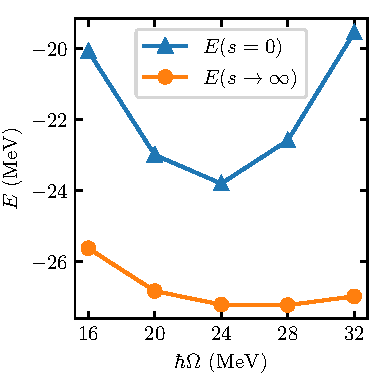
\includegraphics[width=0.45\textwidth]{thesis/doc/images/he4_imsrg2_energies.pdf}
  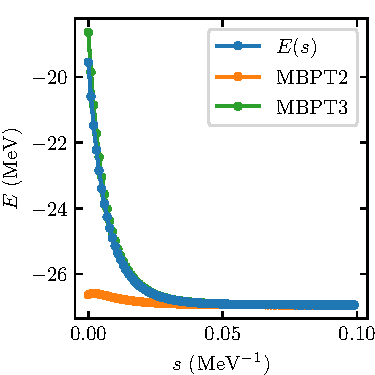
\includegraphics[width=0.45\textwidth]{thesis/doc/images/he4_imsrg2_flow.pdf}
  \caption[
    The left panel shows $E(s=0)$ and $E(s \rightarrow \infty)$
    for an IMSRG(2) calculation of ${}^4\text{He}$
    for $\hbar \Omega$ ranging from $16\mev$ to $32\mev$.
    The interaction used is the EM NN interaction
    with a regulator cutoff $\Lambda=500\mev$
    and SRG-evolved to $\lambda=1.8\invfm$.
    The right panel shows the flowing energy $E(s)$
    along with the energy with second- and third-order MBPT corrections included
    for $\hbar \Omega=32\mev$.
    The right panel is similar for the different $\hbar \Omega$ of the left panel.
  ]{
    The left panel shows $E(s=0)$ and $E(s \rightarrow \infty)$
    for an IMSRG(2) calculation of ${}^4\text{He}$
    for $\hbar \Omega$ ranging from $16\mev$ to $32\mev$.
    The interaction used is the EM NN interaction
    with a regulator cutoff $\Lambda=500\mev$
    and SRG-evolved to $\lambda=1.8\invfm$~\cite{Ente03n3lonn}.
    The right panel shows the flowing energy $E(s)$
    along with the energy with second- and third-order MBPT corrections included
    for $\hbar \Omega=32\mev$.
    The right panel is similar for the different $\hbar \Omega$ of the left panel.
  }\label{fig:imsrg2_he4_results}
\end{figure}

For $\twobodyop{V}$, we use the EM NN potential from Ref.~\cite{Ente03n3lonn} at \nthreelo{}
with a regulator cutoff at $\Lambda=500\mev$ and SRG-evolved to $\lambda=1.8\invfm$.
The results from normal ordering our Hamiltonians at the different $\hbar \Omega$
with respect to our HO reference state
and evaluating the IMSRG(2) evolution are shown
in the left panel of Fig.~\ref{fig:imsrg2_he4_results}.
We find that the unevolved energy $E(s=0)$,
that is, the energy expectation value of the reference state,
is already good to within 30\% of the exact result,
a consequence of the SRG-softened interaction we are using.
Still, the IMSRG evolution absorbs up to $8\mev$ of correlation energy into the ground-state energy.
We also find that our implementation agrees with the implementation from Ref.~\cite{Stro15imsrgcpp}
to within $10^{-5}\mev$.

In the right panel of Fig.~\ref{fig:imsrg2_he4_results},
we show the flowing ground-state energy
as well as the ground-state energy with second- and third-order MBPT corrections.
We find that these corrections vanish as the correlations are absorbed into the ground-state energy,
indicating that we are achieving the desired decoupling.
We emphasize once again that these results are intended to be interpreted as validation
(for example, as a nuclear-like toy model)
and not as physically meaningful.
We consider the agreement between our implementation and that of Ref.~\cite{Stro15imsrgcpp}
to be \textit{a posteriori} evidence of the correctness of our implementation.


\chapter{Angular-momentum coupling for the IMSRG}\label{ch:ang_mom_coupling}

In theoretical physics,
the exploitation of symmetries is essential to making
the solution of certain problems computationally tractable.
In many-body theories,
general theories can be simplified
(in terms of computational cost)
by exploiting the symmetries
present in the system and the chosen single-particle basis.
For rotationally invariant systems,
this symmetry exploitation is called angular-momentum reduction (AMR),
which casts the many-body problem
into the language of spherical tensors
and angular-momentum eigenstates
and analytically simplifies
the angular-momentum-projection dependence
related to the geometry of spherical systems.
The angular-momentum reduction of a many-body approach
can reduce the storage and computational cost by orders of magnitude,
making it a very powerful tool to extend
the range of the approach to larger model spaces
or in some cases make calculations possible at all.
The IMSRG is an excellent target for angular-momentum reduction,
as one typically needs to push the model space
to quite large single-particle basis truncations
to achieve converged results.
In this chapter,
we give a brief overview of how angular-momentum reduction works
and discuss its application
to the IMSRG(3).

\section{Wigner-Eckart theorem}\label{sec:amr}

Core to the angular-momentum reduction formalism
are rotational symmetry,
formally described by the SU(2) Lie group,
and the generator of rotations,
the angular momentum $\vec{J}$.
The prerequisites for AMR are~\cite{Tich20jcoupling}:
a rotationally invariant Hamiltonian, which commutes with $\vec{J}$;
a spherical single-particle basis, which consists of eigenstates of $J^2$ and $J_{z}$;
and a spherical reference state,
which has good angular momentum $J=0$.
In this case, the Hamiltonian, the single-particle basis,
and the reference state share the symmetry group SU(2),
and one can cast the working equations of the theory
into a spherically symmetric form
and perform the analytical simplifications
to allow one to profit from AMR.

An operator $O$ can be expanded in spherical tensors $\mathbf{O}^{J}$ of rank $J$,
each with $2 J + 1$ components $O^{J}_{M}$~\cite{Suho07angmom}.
These spherical tensors have definite transformation behavior
under rotations.
Specifically, for a given unitary transformation $U(R)$
that corresponds to a rotation $R$,
the spherical tensor components transform like~\cite{Suho07angmom}
\begin{equation}
  U(R)O^{J}_{M}U^{\dagger}(R) = \sum_{M'=-J}^{J} D^{J}_{M'M}(R) O_{M'}^{J}\,,
\end{equation}
where $D^{J}_{M'M}(R)$ are the Wigner $D$ functions,
which also give the transformation of the spherical harmonics under the same rotation~\cite{Suho07angmom}:
\begin{equation}
  U(R)\ket{j m} = \sum_{m' = -j}^{j} D_{m' m}^{j}(R) \ket{j m'}.
\end{equation}
Spherical tensors can be further simplified by the Wigner-Eckart theorem.
The Wigner-Eckart theorem states
that the matrix elements of a spherical tensor
can be factorized into
a reduced matrix element that is operator-specific
and independent of any angular-momentum projection
(in the bra state, ket state, and the tensor component)
and a projection-dependent part
that contains only geometric information
and is independent of the specific operator~\cite{Wign27wet,Ecka30wet}:
\begin{equation}\label{eq:wet_theorem}
  \braket{\xi_1 j_1 m_1 | O^{J}_{M} | \xi_2 j_2 m_2 }
  = (-1 )^{2J} \frac{1}{\hat{\jmath}_1}
  \cgsymbol{j_2}{J}{j_1}{m_2}{M}{m_1}
  \braket{\xi_1 j_1 || \textbf{O}^{J} || \xi_2 j_2}\,,
\end{equation}
where $\hat{\jmath} \equiv \sqrt{2 j + 1}$.
The states $\ket{\xi j m}$
are eigenstates of
angular momentum squared $J^2$
and angular-momentum projection $J_{z}$,
with all other relevant quantum numbers
contained in $\xi$.
We generally use the shorthand $\ket{p} = \ket{\tilde{p} m_p}$,
where $\tilde{p} \equiv \xi_p j_p$, for simplicity.
Occasionally, we need time-reversed states
with flipped angular-momentum projections,
which we denote by $\ket{\bar{p}} \equiv \ket{\tilde{p} (-m_p)}$.
Note that the reduced single-particle index $\tilde{p}$ is the same
for normal states and time-reversed states.
Note that in Eq.~\eqref{eq:wet_theorem}
we have chosen the ``Wigner'' convention for reduced matrix elements,
which is also used by Suhonen, Edmonds, Racah, and Varshalovich
and which differs from the convention used by, for example, Sakurai.

Equipped with the factorization
provided by the Wigner-Eckart theorem
and the choice of spherical reference state
and single-particle basis,
one can in principle analytically perform the summations
over all the angular-momentum-projection quantum numbers
in a given expression.
Intuitively,
for every reduced index $\tilde{p}$ in a many-body expression,
one knows that both the reduced matrix elements
and the reference state do not depend on $m_p$,
so one is able to treat the entire ``shell''
of $2 j_p + 1$ states collectively.
This is where the ``reduction'' part of angular-momentum reduction
takes place,
since the resulting expressions
are completely independent of projection quantum numbers,
and one can use a reduced representation
for the remaining operator-specific information
that does not depend on the projection quantum numbers.

One particularly convenient approach to
doing angular-momentum reduction
is the diagrammatic expansion
of an expression in a so-called Jucys graph
and the simplification of the graph using various identities~\cite{Vars88angmom,Worm06angmom,Lind86angmom}.
This approach was automated in the \texttt{amc} code
published in Ref.~\cite{Tich20jcoupling}.
The \texttt{amc} program
automatically converts an uncoupled expression
provided to it via an input file written in the AMC language
into an equivalent $m$-independent reduced expression.
Accomplishing this reduction by hand
is tedious and error-prone,
so we used this program as the primary workhorse
for the angular-momentum reduction in Section~\ref{sec:amr_scalar}.

\section{Angular-momentum reduction for scalar operators}\label{sec:amr_scalar}

We will now apply angular-momentum reduction
to the in-medium similarity renormalization group.
The result of this symmetry reduction is the so-called $J$-scheme IMSRG,
where the flow equations are formulated
in terms of coupled or reduced matrix elements
and the expressions have been reduced
such that all dependence on angular-momentum projections
has been analytically simplified.
In the nuclear case,
scalar operators play a special role in the IMSRG
as the Hamiltonian and the generator are both scalar operators.
This means that the many-body formalisms
discussed in Chapters~\ref{ch:many_body} and~\ref{ch:imsrg}
can be symmetry reduced for closed-shell systems
by considering only the case of scalar spherical tensors.
As a result,
the $J$-scheme IMSRG can access energies and charge radii
without needing to consider the more complicated case
of general spherical tensor operators
(which we give an outlook on in Section~\ref{sec:tensor_jscheme}).

\subsection{Operator representation}

Since spherical scalars are invariant under rotations
and do not depend on any angular-momentum projection numbers,
one can work with coupled matrix elements
rather than reduced matrix elements
  [as in Eq.~\eqref{eq:wet_theorem}],
which differ by a simple factor
(shown here for a one-body operator):
\begin{equation}
  \braket{\tilde{p} | T^{0}_{0} | \tilde{q}} =
  \frac{1}{\hat{j_p}}\braket{\tilde{p} || \mathbf{T}^{0} || \tilde{q}}.
\end{equation}

For the IMSRG(3), we need coupled matrix elements
for up to three-body operators.
Thus, we need to couple our $A$-body basis
to be made up of eigenstates of
the $A$-body total angular momentum squared $J^2$
and the $z$-component of the total angular momentum $J_{z}$.
Since our chosen single-particle basis $\ket{p} = \ket{\tilde{p}m_p}$
consists of eigenstates of $J_{\text{1B}}^2$ and $J_{\text{1B},z}$
for the one-body angular momentum $\vec{J}_{\text{1B}}$,
the coupled matrix elements of a scalar one-body operator
are simply the uncoupled matrix elements
\footnote{
  In Eq.~\eqref{eq:onebody_coupled_to_uncoupled},
  $p$ and $q$ have their angular-momentum projections
  implicitly fixed to $m_p=m_q=1/2$.
},
\begin{equation}
  O_{\tilde{p} \tilde{q}} = \braket{\tilde{p} m_p=1/2 | O | \tilde{q} m_q=1/2} \delta_{j_p j_q}
  = O_{pq}\,, \label{eq:onebody_coupled_to_uncoupled}
\end{equation}
where we have explicitly denoted that $O$ is diagonal in $j_p$
\footnote{We previously denoted $A$-body operators by $\abodyop{O}$.
  From this point on, we will leave off the (redundant) superscript
  to reduce notational clutter,
  as the many-body rank of an operator
  can be inferred from the number of indices on its matrix elements.}.
Note that $m_p = m_q$ could be any other value
within the range given by $j_p$;
the matrix elements of a scalar operator will not change due to a different choice.
We used $m_p=1/2$ here simply because it will always be a valid choice
for all $j_p$ in our single-particle basis.

The representation of one-body operators can be made a bit more clear
by adding an angular-momentum ``channel'' to the notation:
\begin{equation}
  O^{j}_{pq}\,.
\end{equation}
The channel $j$ indicates that the matrix elements of $O_{pq}$
are diagonal in $j_p=j_q$,
and in this channel only the indices $p$ and $q$ with
$j_p = j_q = j$ have non-zero matrix elements.
We will stick with this notation
for coupled one-body matrix elements going forward.

Our antisymmetrized two-body states
\begin{equation}
  \ket{pq} = \crea{p} \crea{q} \ket{0}
\end{equation}
are not eigenstates of $J_{\text{2B}}^2$,
only of $J_{\text{2B},z}$.
Coupling the states to two-body angular momentum $J_{pq}$
gives the coupled two-body basis,
\begin{equation}\label{eq:unnormalized_twobody_basis}
  \ket{(\tilde{p} \tilde{q}) J_{pq} M_{pq}} \equiv
  \sum_{m_p, m_q}
  \cgsymbol{j_p}{j_q}{J_{pq}}{m_p}{m_q}{M_{pq}}
  \ket{pq}
  \,,
\end{equation}
where the coupling brackets in $\ket{(\tilde{p} \tilde{q}) J_{pq} M_{pq}}$
indicate that $j_p$ and $j_q$ are coupled to $J_{pq}$
(and the rest of the quantum numbers in $\tilde{p}$ and $\tilde{q}$ are not involved).
Note that the Clebsch-Gordan coefficients
\begin{equation}
  \cgsymbol{j_p}{j_q}{J_{pq}}{m_p}{m_q}{M_{pq}}
\end{equation}
are defined such that they are 0
if $M_{pq} \neq m_p + m_q$,
collapsing one of the sums over angular-momentum projections.
The two-body states in Eq.~\eqref{eq:unnormalized_twobody_basis}
are not normalized,
which can be remedied by multiplying them with the following factor~\cite{Suho07angmom}:
\begin{equation}
  N_{pq(J_{pq})} \equiv \frac{\sqrt{1 + (-1)^{J_{pq}}
      \delta_{\tilde{p} \tilde{q}}}}{1 + \delta_{\tilde{p} \tilde{q}}}.
\end{equation}
However, the coupled many-body expressions
(and their numerical implementations)
are simpler when using unnormalized coupled two- and three-body matrix elements.

The unnormalized coupled two-body matrix elements of
a scalar two-body operator $O$ are given by
\begin{samepage}
  \begin{align}
    O^{J_{pq}}_{\tilde{p}\tilde{q}\tilde{r}\tilde{s}}
     & \equiv \braket{
      (\tilde{p} \tilde{q})J_{pq} M_{pq}=0|
      O
      |(\tilde{r} \tilde{s})J_{pq} M_{pq}=0
    }                           \\
     & =\sum_{\substack{m_p,m_q \\ m_r,m_s}}
    \cgsymbol{j_p}{j_q}{J_{pq}}{m_p}{m_q}{M_{pq} = 0}
    \cgsymbol{j_r}{j_s}{J_{pq}}{m_r}{m_s}{M_{pq} = 0}
    O_{pqrs}\,.\label{eq:unnormalized_twobody_mels}
  \end{align}
\end{samepage}
Our representation builds the diagonality of the matrix elements
in $J_{pq} = J_{rs}$ into the notation,
as indicated by the $J_{pq}$ channel in the superscript.
Again, $M_{pq} = 0$ is a choice we have made that works
for all sets of $\tilde{p}$ and $\tilde{q}$.
It is worth noting that not all $\tilde{p} \tilde{q}$
(or $\tilde{r} \tilde{s}$) combinations
can couple to a given $J_{pq}$.
This is not a problem, because in Eq.~\eqref{eq:unnormalized_twobody_mels}
the Clebsch-Gordan coefficients cause those matrix elements to be 0.
This means they do not unphysically contribute in any many-body expressions.
In numerical implementations,
the exploitation of this reduction in the number of valid two-body states
in a given angular-momentum channel
is essential to improving performance to the point
where calculations in large model spaces are possible.

The definition of the coupled three-body basis follows analogously,
\begin{equation}\label{eq:unnormalized_threebody_basis}
  \ket{[(\tilde{p} \tilde{q}) J_{pq} \tilde{r}] J_{pqr} M_{pqr}} \equiv
  \sum_{m_r, M_{pq}}
  \cgsymbol{J_{pq}}{j_r}{J_{pqr}}{M_{pq}}{m_r}{M_{pqr}}
  \sum_{m_p, m_q}
  \cgsymbol{j_p}{j_q}{J_{pq}}{m_p}{m_q}{M_{pq}}
  \ket{pqr}
  \,,
\end{equation}
where we have selected the ``standard'' coupling order
with $j_p$ and $j_q$ coupled first to $J_{pq}$
and then $J_{pq}$ and $j_r$ coupled to $J_{pqr}$.
Once again, these states are not normalized,
but working with unnormalized states is more convenient.

The unnormalized coupled matrix elements of a three-body operator $O$
are given by
\begin{align}
  \phantom{O^{(J_{pqr}, J_{pq}, J_{st})}_{\tilde{p}\tilde{q}\tilde{r}\tilde{s}\tilde{t}\tilde{u}}}
   & \begin{aligned}
    \mathllap{O^{(J_{pqr}, J_{pq}, J_{st})}_{\tilde{p}\tilde{q}\tilde{r}\tilde{s}\tilde{t}\tilde{u}}}
    \equiv \braket{
    [(\tilde{p} \tilde{q})J_{pq} \tilde{r}] J_{pqr} M_{pqr} = 1/2 |
    O
    | [(\tilde{s} \tilde{t})J_{st} \tilde{u}] J_{pqr} M_{pqr} = 1/2
    }
  \end{aligned} \\
   & \begin{aligned}
    \mathllap{}
    = \sum_{\substack{m_p,m_q,m_r,M_{pq}                     \\ m_s,m_t,m_u,M_{st}}} &
    \cgsymbol{j_p}{j_q}{J_{pq}}{m_p}{m_q}{M_{pq}}
    \cgsymbol{j_s}{j_t}{J_{st}}{m_s}{m_t}{M_{st}}            \\
     & \cgsymbol{J_{pq}}{j_r}{J_{pqr}}{M_{pq}}{m_r}{M_{pqr}=1/2}
    \cgsymbol{J_{st}}{j_u}{J_{pqr}}{M_{st}}{m_u}{M_{pqr}=1/2}    \\
     & O_{pqrstu}
    \,.
  \end{aligned}
\end{align}
The channel structure of the three-body matrix elements
has grown more complicated,
with the channel including the diagonal total three-body angular momentum
$J_{pqr} = J_{stu}$
and the intermediate couplings $J_{pq}$ and $J_{st}$.
These intermediate couplings can take on different values,
substantially increasing the number of three-body channels
for which we need to handle matrix elements.
Again, $M_{pqr} = 1/2$ is a choice we have made that works
for all sets of $\tilde{p}$, $\tilde{q}$, and $\tilde{r}$.

At this point, it is useful to discuss the symmetry properties
of these matrix elements.
For a Hermitian operator
the coupled matrix elements have the following properties:
\begin{samepage}
  \begin{subequations}
    \begin{align}
      O_{\tilde{p}\tilde{q}}                                                                 & = O_{\tilde{q}\tilde{p}}\,, \\
      O^{J_{pq}}_{\tilde{p}\tilde{q}\tilde{r}\tilde{s}}                                      & =
      O^{J_{pq}}_{\tilde{r}\tilde{s}\tilde{p}\tilde{q}}\,,                                                                 \\
      O^{(J_{pqr}, J_{pq}, J_{st})}_{\tilde{p}\tilde{q}\tilde{r}\tilde{s}\tilde{t}\tilde{u}} & =
      O^{(J_{pqr}, J_{st}, J_{pq})}_{\tilde{s}\tilde{t}\tilde{u}\tilde{p}\tilde{q}\tilde{r}}\,.\label{eq:coupled_herm_threebody}
    \end{align}
  \end{subequations}
\end{samepage}
Note the transposition of the intermediate couplings
in the three-body channel in Eq.~\eqref{eq:coupled_herm_threebody}.
For an anti-Hermitian operator
the coupled matrix elements have the following properties:
\begin{subequations}
  \begin{align}
    O_{\tilde{p}\tilde{q}}                                                                 & = - O_{\tilde{q}\tilde{p}}\,, \\
    O^{J_{pq}}_{\tilde{p}\tilde{q}\tilde{r}\tilde{s}}                                      & =
    - O^{J_{pq}}_{\tilde{r}\tilde{s}\tilde{p}\tilde{q}}\,,                                                                 \\
    O^{(J_{pqr}, J_{pq}, J_{st})}_{\tilde{p}\tilde{q}\tilde{r}\tilde{s}\tilde{t}\tilde{u}} & =
    - O^{(J_{pqr}, J_{st}, J_{pq})}_{\tilde{s}\tilde{t}\tilde{u}\tilde{p}\tilde{q}\tilde{r}}\,.\label{eq:coupled_antiherm_threebody}
  \end{align}
\end{subequations}

Our two- and three-body matrix elements are also antisymmetric,
although this symmetry is not realized as simply
for coupled matrix elements as it is for uncoupled matrix elements.
Two-body matrix elements have the following properties:
\begin{subequations}
  \begin{align}
    O_{\tilde{p}\tilde{q}\tilde{r}\tilde{s}}^{J_{pq}} & =
    - (-1)^{j_p + j_q - J_{pq}}
    O_{\tilde{q}\tilde{p}\tilde{r}\tilde{s}}^{J_{pq}}\,,  \\
    O_{\tilde{p}\tilde{q}\tilde{r}\tilde{s}}^{J_{pq}} & =
    - (-1)^{j_r + j_s - J_{pq}}
    O_{\tilde{p}\tilde{q}\tilde{s}\tilde{r}}^{J_{pq}}\,.
  \end{align}
\end{subequations}
Three-body matrix elements have the following properties:
\begin{subequations}
  \begin{align}
    O_{\tilde{p}\tilde{q}\tilde{r}\tilde{s}\tilde{t}\tilde{u}}^{(J_{pqr}, J_{pq}, J_{st})} & =
    - (-1)^{j_p + j_q - J_{pq}}
    O_{\tilde{q}\tilde{p}\tilde{r}\tilde{s}\tilde{t}\tilde{u}}^{(J_{pqr}, J_{pq}, J_{st})}\,,  \\
    O_{\tilde{p}\tilde{q}\tilde{r}\tilde{s}\tilde{t}\tilde{u}}^{(J_{pqr}, J_{pq}, J_{st})} & =
    \hat{J}_{pq}
    \sum_{J_{2}} \hat{J}_{2}
    \sixj{j_p}{j_q}{J_{pq}}{j_r}{J_{pqr}}{J_{2}}
    O_{\tilde{r}\tilde{q}\tilde{p}\tilde{s}\tilde{t}\tilde{u}}^{(J_{pqr}, J_{2}, J_{st})}\,,   \\
    O_{\tilde{p}\tilde{q}\tilde{r}\tilde{s}\tilde{t}\tilde{u}}^{(J_{pqr}, J_{pq}, J_{st})} & =
    - (-1)^{j_q + j_r - J_{pq}}
    \hat{J}_{pq}
    \sum_{J_{2}} \hat{J}_{2} (-1)^{J_{2}}
    \sixj{j_q}{j_p}{J_{pq}}{j_r}{J_{pqr}}{J_{2}}
    O_{\tilde{p}\tilde{r}\tilde{q}\tilde{s}\tilde{t}\tilde{u}}^{(J_{pqr}, J_{2}, J_{st})}\,,   \\
    O_{\tilde{p}\tilde{q}\tilde{r}\tilde{s}\tilde{t}\tilde{u}}^{(J_{pqr}, J_{pq}, J_{st})} & =
    - (-1)^{j_s + j_t - J_{st}}
    O_{\tilde{p}\tilde{q}\tilde{r}\tilde{t}\tilde{s}\tilde{u}}^{(J_{pqr}, J_{pq}, J_{st})}\,,  \\
    O_{\tilde{p}\tilde{q}\tilde{r}\tilde{s}\tilde{t}\tilde{u}}^{(J_{pqr}, J_{pq}, J_{st})} & =
    \hat{J}_{st}
    \sum_{J_{2}} \hat{J}_{2}
    \sixj{j_s}{j_t}{J_{st}}{j_u}{J_{pqr}}{J_{2}}
    O_{\tilde{p}\tilde{q}\tilde{r}\tilde{u}\tilde{t}\tilde{s}}^{(J_{pqr}, J_{pq}, J_{2})}\,,   \\
    O_{\tilde{p}\tilde{q}\tilde{r}\tilde{s}\tilde{t}\tilde{u}}^{(J_{pqr}, J_{pq}, J_{st})} & =
    - (-1)^{j_t + j_u - J_{st}}
    \hat{J}_{st}
    \sum_{J_{2}} \hat{J}_{2} (-1)^{J_{2}}
    \sixj{j_t}{j_s}{J_{st}}{j_u}{J_{pqr}}{J_{2}}
    O_{\tilde{p}\tilde{q}\tilde{r}\tilde{s}\tilde{u}\tilde{t}}^{(J_{pqr}, J_{pq}, J_{2})}\,.
  \end{align}
\end{subequations}
We provide only the pairwise antisymmetry properties,
as the relations for the remaining permutations
can be obtained by applying pairwise permutations.

At this point, we drop the cumbersome ``tilde'' notation
for reduced state indices.
The channels on matrix elements should make it clear
whether the matrix elements are coupled or not.
Additionally, in the surrounding text,
we make it clear whether an expression
is coupled or uncoupled.

\subsection{Coupled many-body expressions}\label{sec:jscheme_many_body_expressions}

In addition to the fundamental commutators,
IMSRG calculations typically employ a couple standard operations,
which we discuss here.
The first is bringing the initial Hamiltonian into normal order
with respect to the employed $A$-body reference state.
Given a Hamiltonian $H$ with one- through three-body parts,
the coupled expressions for
the matrix elements of the normal-ordered Hamiltonian are
\begin{subequations}
  \begin{align}
    \phantom{W_{pqrstu}^{(J_{pqr}, J_{pq}, J_{st})}}
     & \begin{aligned}
      \mathllap{E} = \bar{H} & = \sum_{j_{a}} \hat{\jmath}^{2}_a \sum_{a} H_{aa}^{j_{a}}
      + \frac{1}{2} \sum_{J_{ab}} \hat{J}_{ab}^2 \sum_{ab} H_{abab}^{J_{ab}}             \\
                             & \quad
      + \frac{1}{6} \sum_{J_{ab} J_{abc}} \hat{J}_{abc}^2 \sum_{abc}  H_{abcabc}^{(J_{abc}, J_{ab}, J_{ab})}\,,
    \end{aligned} \\
     & \begin{aligned}
      \mathllap{f_{pq}^{j_p}} = \bar{H}_{pq}^{j_p} &
      = H_{pq}^{j_p}
      + \frac{1}{\hat{\jmath}_{p}^2} \sum_{J_{pa}} \hat{J}_{pa}^2 \sum_{a} H_{paqa}^{J_{pa}} \\
                                                   & \quad
      + \frac{1}{2 \hat{\jmath}_{p}^2} \sum_{J_{pa} J_{pab}} \hat{J}_{pab}^2 \sum_{ab}  H_{pabqab}^{(J_{pab}, J_{pa}, J_{pa})}\,,
    \end{aligned} \\
     & \begin{aligned}
      \mathllap{\Gamma_{pqrs}^{J_{pq}}} = \bar{H}_{pqrs}^{J_{pq}}
       & = H_{pqrs}^{J_{pq}}
      + \frac{1}{\hat{J}_{pq}^2} \sum_{J_{pqa}} \hat{J}_{pqa}^2 \sum_{a} H_{pqarsa}^{(J_{pqa}, J_{pq}, J_{pq})} \,,
    \end{aligned} \\
     & \begin{aligned}
      \mathllap{W_{pqrstu}^{(J_{pqr}, J_{pq}, J_{st})}} = \bar{H}_{pqrstu}^{(J_{pqr}, J_{pq}, J_{st})} & = H_{pqrstu}^{(J_{pqr}, J_{pq}, J_{st})} \,.
    \end{aligned}
  \end{align}
\end{subequations}
Recall our previous convention that
the indices $p$, $q$, $r$, \ldots\ run over all single-particle states,
the indices $i$, $j$, $k$, \ldots\ run over hole states,
and the indices $a$, $b$, $c$, \ldots\ run over particle states.

Next, we need an antisymmetrizer for our two- and three-body matrix elements.
This is because the fundamental commutators in Section~\ref{sec:jscheme_fundamental_comm}
are not antisymmetrized to simplify the expressions and the numerical implementations.
Thus, we need to explicitly restore the antisymmetry of some index combinations
after evaluating the non-antisymmetrized fundamental commutators.
In the two-body case,
the antisymmetrizer is
\begin{equation}\label{eq:twobody_antisymmetrizer}
  \mathcal{A}_{\text{2B}} \equiv\mathcal{A}_{pq} \mathcal{A}_{rs}\,,
\end{equation}
with
\begin{equation}
  \mathcal{A}_{pq} \equiv \frac{1}{2}(1 - P_{pq})\,.
\end{equation}
Recall that in the uncoupled expressions in Chapter~\ref{ch:imsrg}
the permutation operator $P_{pq}$ simply exchanged the indices $p$ and $q$ in the following expression.
Now that indices are coupled,
the action of permutation operators is complicated
by the fact that they also change the coupling order.
To implement $\mathcal{A}_{\text{2B}}$,
all we need are the expressions for the action of $P_{pq}$
and $P_{rs}$ on two-body matrix elements:
\begin{subequations}
  \begin{align}
    O_{pqrs}^{J_{pq}} & \xleftarrow{P_{pq}} (-1)^{j_p + j_q - J_{pq}} O_{qprs}^{J_{pq}}\,, \\
    O_{pqrs}^{J_{pq}} & \xleftarrow{P_{rs}} (-1)^{j_r + j_s - J_{pq}} O_{pqsr}^{J_{pq}}\,.
  \end{align}
\end{subequations}
Using these operations along with scalar multiplication of and addition of matrix elements,
the implementation of a two-body antisymmetrizer is simple.

In the three-body case,
the antisymmetrizer is
\begin{equation}\label{eq:threebody_antisymmetrizer}
  \mathcal{A}_{\text{3B}} \equiv \mathcal{A}_{pqr} \mathcal{A}_{stu}\,,
\end{equation}
with
\begin{equation}
  \mathcal{A}_{pqr} \equiv \frac{1}{6}(1 + P_{prq} + P_{prq}^2)(1 - P_{pq})\,.
\end{equation}
Here $P_{prq}$ cyclically permutes the indices $p$, $q$, and $r$ such that
\begin{equation}
  (p, q, r) \xrightarrow{P_{prq}} (q, r, p) \xrightarrow{P_{prq}} (r, p, q) \xrightarrow{P_{prq}} (p, q, r)\,.
\end{equation}
There are other ways to define $\mathcal{A}_{pqr}$,
for example in terms of $P_{pq}$ and $P_{qr}$.
They are all equivalent,
and which one one chooses is a matter of preference.
The action of $P_{prq}$, $P_{pq}$, $P_{sut}$, and $P_{st}$
on three-body matrix elements is given by
\begin{subequations}
  \begin{align}
    O_{pqrstu}^{(J_{pqr}, J_{pq}, J_{st})} &
    \xleftarrow{P_{prq}}
    -1 (-1)^{j_p + j_q - J_{pq}} \hat{J}_{pq}
    \sum_{J_{2}} \hat{J}_{2}
    \sixj{j_q}{j_p}{J_{pq}}{j_r}{J_{pqr}}{J_{2}}
    O_{rpqstu}^{(J_{pqr}, J_{2}, J_{st})}\,,  \\
    O_{pqrstu}^{(J_{pqr}, J_{pq}, J_{st})} &
    \xleftarrow{P_{pq}}
    (-1)^{j_p + j_q - J_{pq}}
    O_{qprstu}^{(J_{pqr}, J_{pq}, J_{st})}\,, \\
    O_{pqrstu}^{(J_{pqr}, J_{pq}, J_{st})} &
    \xleftarrow{P_{sut}}
    -1 (-1)^{j_s + j_t - J_{st}} \hat{J}_{st}
    \sum_{J_{2}} \hat{J}_{2}
    \sixj{j_t}{j_s}{J_{st}}{j_u}{J_{pqr}}{J_{2}}
    O_{pqrust}^{(J_{pqr}, J_{pq}, J_{2})}\,,  \\
    O_{pqrstu}^{(J_{pqr}, J_{pq}, J_{st})} &
    \xleftarrow{P_{st}}
    (-1)^{j_s + j_t - J_{st}}
    O_{pqrtsu}^{(J_{pqr}, J_{pq}, J_{st})}\,.
  \end{align}
\end{subequations}
With these basic operations in hand,
one can implement a general three-body antisymmetrizer.

Finally, the second-order M{\o}ller-Plesset MBPT (MP2) energy correction
is a critical diagnostic for the IMSRG
as it is directly proportional to the matrix elements
that the IMSRG evolution should suppress.
The coupled expression for the MP2 energy correction is
\begin{equation}
  E_{\text{MP2}} =
  - \sum_{j_{a}} \hat{\jmath}_{a}^2 \sum_{ai} \frac{|f_{ai}^{j_a}|^2}{\epsilon_{i}^{a}}
  - \frac{1}{4} \sum_{J_{ab}} \hat{J}_{ab}^2 \sum_{abij}
  \frac{|\Gamma_{abij}^{J_{ab}}|^2}{\epsilon_{ij}^{ab}}
  - \frac{1}{36} \sum_{J_{abc} J_{ab} J_{ij}} \hat{J}_{abc}^2 \sum_{abcijk}
  \frac{|W_{abcijk}^{(J_{abc}, J_{ab}, J_{ij})}|^2}{\epsilon_{ijk}^{abc}}\,,
\end{equation}
with
\begin{align}
  \epsilon_{ij\cdots}^{ab\cdots} & = e_a + e_b + \cdots - (e_i + e_j + \cdots)\,, \\
  e_p                            & = f_{pp}\,,
\end{align}
as in Eq.~\eqref{eq:mp_energy_denom}.

\subsection{Coupled fundamental commutators}\label{sec:jscheme_fundamental_comm}

In this section,
we present the coupled expressions for
the fundamental commutators of two scalar operators.
These expressions were obtained using
the \texttt{amc} code from Ref.~\cite{Tich20jcoupling}
on the uncoupled commutator expressions
given in Appendix~\ref{app:mscheme_fundamental_commutators}.
While this approach immediately produced desirable results
for some commutators,
for many it was possible to simplify the resulting expressions
by exploiting symmetries of the uncoupled expressions.
We discuss examples of these simplifications in Appendix~\ref{app:jscheme_commutator_tricks}.
Here, we will only show the simplest expressions
we were able to produce.

The commutator expressions are ``fundamental'' in the sense
that they are the basic operations required for any IMSRG(3) implementation.
Using these expressions,
one can quickly combine and expand them to produce
the full IMSRG(3) flow equations (see Section~\ref{sec:imsrgthree}),
and one can also easily implement
the series of nested commutators required by
the Magnus and BCH expansions (see Section~\ref{sec:imsrg_magnus}).
Thus, correctly and efficiently implementing these expressions
constitutes the main challenge of any IMSRG implementation.

The commutator of a $K$-body and an $L$-body operator
gives an operator with \mbox{$|K-L|$-} to $(K+L-1)$-body parts:
\begin{equation}
  \left[A^{(K)}, B^{(L)}\right] = \sum_{M=|K - L|}^{K + L - 1} C^{(M)}\,.
\end{equation}
The expressions we give below are
for the coupled matrix elements of the different $M$-body terms.
In the IMSRG(3), we discard any four- and five-body parts induced,
which appear in principle
in the commutator of a two-body and a three-body operator
and in the commutator of two three-body operators.
We focus on the case where $A$ and $B$ and thus the resulting $C$ are scalar operators.

Note that expressions for two- and three-body matrix elements
are not antisymmetrized,
so the appropriate antisymmetrizer must be applied
  [see Eqs.~\eqref{eq:twobody_antisymmetrizer} and~\eqref{eq:threebody_antisymmetrizer}]
to the matrix elements after evaluating the commutator.
We break our typical index label convention
to use the convention that the index labels $i$,~$j$,~$k$,~\ldots\
are reserved for external indices,
that is, indices appearing on the matrix elements of the resulting operator,
and the index labels $a$,~$b$,~$c$,~\ldots\
are reserved for contracted indices,
that is, indices that are summed over in the matrix elements of the input operators.
As in Chapter~\ref{ch:imsrg}, $\bar{n}_a = 1 - n_a$.

\subsubsection{
  \texorpdfstring{$[\onebodyop{A}, \onebodyop{B}]$}{[1, 1]}
}

The commutator of two one-body operators has
zero- and one-body parts.

The resulting zero-body contribution is given by the coupled expression
\begin{equation}
  C = \sum_{j_a} \hat{\jmath}^{2}_{a} \sum_{ab} (n_a - n_b) A_{ab}^{j_a} B_{ba}^{j_a}\,.
\end{equation}

The resulting coupled one-body matrix elements are given by the coupled expression
\begin{equation}
  C_{ij}^{j_i} = \sum_{a}(A_{ia}^{j_i} B_{aj}^{j_i} - B_{ia}^{j_i} A_{aj}^{j_i})\,.
\end{equation}

\subsubsection{
  \texorpdfstring{$[\onebodyop{A}, \twobodyop{B}]$}{[1, 2]}
}

The commutator of a one-body operator and a two-body operator has
one- and two-body parts.

The resulting coupled one-body matrix elements are given by the coupled expression
\begin{equation}
  C_{ij}^{j_i} = \frac{1}{\hat{\jmath}_{i}^2} \sum_{j_a} \sum_{J_2} \hat{J}_{2}^2
  \sum_{ab} (n_a \bar{n}_b - \bar{n}_a n_b) A_{ab}^{j_a} B_{iajb}^{J_2}\,.
\end{equation}

The resulting coupled two-body matrix elements are given by the coupled expression
\begin{equation}
  C_{ijkl}^{J_C} = 2 \sum_{j_a} \sum_{a} \left(
  A_{ia}^{j_a} B_{ajkl}^{J_C} - A_{ak}^{j_a} B_{ijal}^{J_C}
  \right)
  \,.
\end{equation}

\subsubsection{
  \texorpdfstring{$[\twobodyop{A}, \twobodyop{B}]$}{[2, 2]}
}

The commutator of two two-body operators has
zero- through three-body parts.

The resulting zero-body contribution is given by the coupled expression
\begin{equation}
  C = \frac{1}{4}\sum_{J_{ab}} \hat{J}_{ab}^{2}\sum_{abcd}
  (n_a n_b \bar{n}_c \bar{n}_d - \bar{n}_a \bar{n}_b n_c n_d)
  A_{abcd}^{J_{ab}} B_{cdab}^{J_{ab}}\,.
\end{equation}

The resulting coupled one-body matrix elements are given by the coupled expression
\begin{equation}
  C_{ij}^{j_i} = \frac{1}{2} \frac{1}{\hat{\jmath}_{i}^2}
  \sum_{J_{ab}} \hat{J}_{ab}^2
  \sum_{abc}
  (\bar{n}_a \bar{n}_b n_c + n_a n_b \bar{n}_c)
  (A_{ciab}^{J_{ab}} B_{abcj}^{J_{ab}} - B_{ciab}^{J_{ab}} A_{abcj}^{J_{ab}})\,.
\end{equation}

The resulting coupled two-body matrix elements are given by the coupled expression
\begin{equation}
  C^{J_C}_{ijkl}
  =
  D^{J_C}_{ijkl}
  + E^{J_C}_{ijkl}\,,
\end{equation}
with
\begin{align}
  D^{J_C}_{ijkl}                        & \equiv \frac{1}{2} \sum_{ab}
  (\bar{n}_a \bar{n}_b - n_a n_b)
  \left(
  A_{ijab}^{J_C} B_{abkl}^{J_C} - B_{ijab}^{J_C} A_{abkl}^{J_C}
  \right)\,,                                                           \\
  \overline{E}_{i\bar{l}k\bar{j}}^{J_C} & \equiv 4 \sum_{ab}
  (n_a \bar{n}_b - \bar{n}_a n_b)
  \overline{A}_{a\bar{b}k\bar{j}}^{J_C}
  \overline{B}_{i\bar{l}a\bar{b}}^{J_C}\,. \label{eq:comm222_term2}
\end{align}
The expression in Eq.~\eqref{eq:comm222_term2} is written
in terms of Pandya-transformed matrix elements,
where the two-body Pandya transformation is given by~\cite{Pand56pandya}
\begin{equation}
  \overline{O}_{p\bar{q}r\bar{s}}^{J_{2}} \equiv
  - \sum_{J_{2}'}
  \hat{J}_{2}^{\prime 2}
  \sixj{j_p}{j_q}{J_{2}}{j_r}{j_s}{J_{2}'}
  O_{prqs}^{J_{2}'}\,.
\end{equation}
The indices $\bar{q}$ and $\bar{s}$ are time reversed,
that is, their angular-momentum projections are flipped.
Since we are working with reduced indices
without angular-momentum projections everywhere,
this distinction is irrelevant,
but we keep the modified indices around to be formally precise.
The Pandya-transformed matrix elements
are useful intermediates that isolate recoupling on $A$, $B$, and $E$
that can be done independently.
The resulting $\overline{E}$ must be
converted back to normal coupled matrix elements
by a final Pandya transformation
before being added to $D$ to give $C$.

The resulting coupled three-body matrix elements are given by the coupled expression
\begin{equation}
  \begin{split}
    C_{ijklmn}^{(J_{C,3}, J_{C,ij}, J_{C,lm})} & =
    -9 (-1)^{J_{C,lm}} \hat{J}_{C,ij} \hat{J}_{C,lm}
    \sum_{a} (-1)^{j_a + j_k}
    \sixj{j_k}{j_a}{J_{C,lm}}{j_{n}}{J_{C,3}}{J_{C,ij}} \\
    & \quad \quad \times \left(
    A_{ijna}^{J_{C,ij}} B_{aklm}^{J_{C,lm}}
    - B_{ijna}^{J_{C,ij}} A_{aklm}^{J_{C,lm}}
    \right).
  \end{split}
\end{equation}

\subsubsection{
  \texorpdfstring{$[\onebodyop{A}, \threebodyop{B}]$}{[1, 3]}
}

The commutator of a one-body operator and a three-body operator has
two- and three-body parts.

The resulting coupled two-body matrix elements are given by the coupled expression
\begin{equation}
  C_{ijkl}^{J_C} = \frac{1}{\hat{J}_{C}^2}
  \sum_{j_a}
  \sum_{J_{B,3}} \hat{J}_{B,3}^2
  \sum_{ab} (n_a \bar{n}_b - \bar{n}_a n_b)
  A_{ab}^{j_a} B_{ijbkla}^{(J_{B,3}, J_{C}, J_{C})}\,.
\end{equation}

The resulting coupled three-body matrix elements are given by the coupled expression
\begin{equation}
  C_{ijklmn}^{(J_{C,3}, J_{C,ij}, J_{C,lm})} =
  3 \sum_{j_a} \sum_{a}
  \left(
  A_{ia}^{j_a} B_{ajklmn}^{(J_{C,3}, J_{C,ij}, J_{C,lm})}
  - A_{la}^{j_a} B_{ijkamn}^{(J_{C,3}, J_{C,ij}, J_{C,lm})}
  \right).
\end{equation}

\subsubsection{
  \texorpdfstring{$[\twobodyop{A}, \threebodyop{B}]$}{[2, 3]}
}

The commutator of a two-body operator and a three-body operator has
one- through three-body parts.

The resulting coupled one-body matrix elements are given by the coupled expression
\begin{equation}
  \begin{split}
    C_{ij}^{j_i} &= - \frac{1}{4} \frac{1}{\hat{\jmath}_{i}^2}
    \sum_{(J_{B,3}, J_{ab})}
    \hat{J}_{B,3}^2
    \sum_{abcd}
    (n_a n_b \bar{n}_c \bar{n}_d - \bar{n}_a \bar{n}_b n_c n_d)
    A_{cdab}^{J_{ab}} B_{abicdj}^{(J_{B,3}, J_{ab}, J_{ab})}\,.
  \end{split}
\end{equation}

The resulting coupled two-body matrix elements are given by the coupled expression
\begin{equation}
  \begin{split}
    C_{ijkl}^{J_C} &= \frac{(-1)^{J_C}}{\hat{J}_C}
    \sum_{J_A, J_{B,3}} \hat{J}_A \hat{J}_{B,3}^2
    \sum_{abc}
    (n_a \bar{n}_b \bar{n}_c + \bar{n}_a n_b n_c) \\
    & \quad \left(
    (-1)^{j_k + j_l}
    \sixj{j_l}{j_k}{J_C}{j_a}{J_{B,3}}{J_A}
    A_{bcak}^{J_A} B_{ijabcl}^{(J_{B,3}, J_C, J_A)}
    \right.\\
    &\quad\quad \left. + (-1)^{j_i + j_j}
    \sixj{j_j}{j_i}{J_C}{j_a}{J_{B,3}}{J_A}
    A_{bcai}^{J_A} B_{klabcj}^{(J_{B,3}, J_C, J_A)}
    \right)\,.
  \end{split}
\end{equation}

The resulting coupled three-body matrix elements are given by the coupled expression
\begin{equation}
  C_{ijklmn}^{(J_{C,3}, J_{C, ij}, J_{C, lm})}
  = D_{ijklmn}^{(J_{C,3}, J_{C, ij}, J_{C, lm})}
  + E_{ijklmn}^{(J_{C,3}, J_{C, ij}, J_{C, lm})}\,,
\end{equation}
with
\begin{align}
  D_{ijklmn}^{(J_{C,3}, J_{C, ij}, J_{C, lm})}
   & \equiv \frac{3}{2} \sum_{ab} (\bar{n}_a \bar{n}_b - n_a n_b)
  A_{ijab}^{J_{C, ij}}
  B_{abklmn}^{(J_{C,3}, J_{C, ij}, J_{C, lm})}\,,                 \\
  E_{ijklmn}^{(J_{C,3}, J_{C,ij}, J_{C,lm})}
   & \equiv
  -\frac{3}{2} \sum_{ab} (\bar{n}_a \bar{n}_b - n_a n_b)
  A_{ablm}^{J_{C, lm}}
  B_{ijkabn}^{(J_{C,3}, J_{C, ij}, J_{C, lm})}\,.
\end{align}

\subsubsection{
  \texorpdfstring{$[\threebodyop{A}, \threebodyop{B}]$}{[3, 3]}
}

The commutator of two three-body operators has
zero- through three-body parts.

The resulting zero-body contribution is given by the coupled expression
\begin{equation}
  C = \frac{1}{36}
  \sum_{(J_3, J_{ab}, J_{de})} \hat{J}_{3}^2
  \sum_{abcdef}
  (
  n_a n_b n_c \bar{n}_d \bar{n}_e \bar{n}_f
  - \bar{n}_a \bar{n}_b \bar{n}_c n_d n_e n_f
  )
  A_{abcdef}^{(J_{3}, J_{ab}, J_{de})}
  B_{defabc}^{(J_{3}, J_{de}, J_{ab})}\,.
\end{equation}

The resulting coupled one-body matrix elements are given by the coupled expression
\begin{equation}
  \begin{split}
    C_{ij}^{j_i} & = \frac{1}{12} \frac{1}{\hat{j}_{i}^2}
    \sum_{(J_{3}, J_{ab}, J_{cd})} \hat{J}_{3}^2
    \sum_{abcde} (
    n_a n_b \bar{n}_c \bar{n}_d \bar{n}_e
    + \bar{n}_a \bar{n}_b n_c n_d n_e
    ) \\
    & \quad \left(
    A_{abicde}^{(J_3, J_{ab}, J_{cd})}
    B_{cdeabj}^{(J_3, J_{cd}, J_{ab})}
    - B_{abicde}^{(J_3, J_{ab}, J_{cd})}
    A_{cdeabj}^{(J_3, J_{cd}, J_{ab})}
    \right).
  \end{split}
\end{equation}

The resulting coupled two-body matrix elements are given by the coupled expression
\begin{equation}
  C_{ijkl}^{J_C}
  = D_{ijkl}^{J_C}
  + E_{ijkl}^{J_C}\,,
\end{equation}
with
\begin{align}
  \phantom{D_{ijkl}^{J_C}}
   & \begin{aligned}
    \mathllap{D_{ijkl}^{J_C}} & \equiv
    \frac{1}{6} \frac{1}{\hat{J}_{C}^2}
    \sum_{(J_3, J_{bc})}
    \sum_{abcd}
    (
    n_a \bar{n}_b \bar{n}_c \bar{n}_d
    - \bar{n}_a n_b n_c n_d
    )                                  \\
                              & \quad
    \left(
    A_{ijabcd}^{(J_3, J_C, J_{bc})} B_{bcdkla}^{(J_3, J_{bc}, J_C)}
    - B_{ijabcd}^{(J_3, J_C, J_{bc})} A_{bcdkla}^{(J_3, J_{bc}, J_C)}
    \right),
  \end{aligned} \\
  \phantom{D_{ijkl}^{J_C}}
   & \begin{aligned}
    \mathllap{E_{ijkl}^{J_C}} & \equiv
    (-1)^{j_j + j_l}
    \sum_{(J_{A,3}, J_{ab}, J_{cd})}
    (-1)^{J_{ab} + J_{cd}} \hat{J}_{A,3}^2
    \sum_{J_{B,3}}
    \hat{J}_{B,3}^2                    \\
                              & \quad
    \ninej{j_i}{J_{A,3}}{J_{ab}}{j_j}{J_{cd}}{J_{B,3}}{J_{C}}{j_l}{j_k}
    \sum_{abcd}
    (
    \bar{n}_a \bar{n}_b n_c n_d
    - n_a n_b \bar{n}_c \bar{n}_d
    )                                  \\
                              & \quad
    A_{abicdk}^{(J_{A,3}, J_{ab}, J_{cd})}
    B_{cdjabl}^{(J_{B,3}, J_{cd}, J_{ab})}\,.
  \end{aligned}
\end{align}

The resulting coupled three-body matrix elements are given by the coupled expression
\begin{equation}
  C_{ijklmn}^{(J_{C,3}, J_{C,ij}, J_{C,lm})}
  = D_{ijklmn}^{(J_{C,3}, J_{C,ij}, J_{C,lm})}
  + E_{ijklmn}^{(J_{C,3}, J_{C,ij}, J_{C,lm})}
  + F_{ijklmn}^{(J_{C,3}, J_{C,ij}, J_{C,lm})}\,,
\end{equation}
with
\begin{align}
  \phantom{D_{ijklmn}^{(J_{C,3}, J_{C,ij}, J_{C,lm})}}
   & \begin{aligned}
    \mathllap{D_{ijklmn}^{(J_{C,3}, J_{C,ij}, J_{C,lm})}}
     & \equiv \frac{1}{6} \sum_{J_{ab}}
    \sum_{ab}
    (n_a n_b n_c + \bar{n}_a \bar{n}_b \bar{n}_c)
    \\
     & \quad \left(
    A_{ijkabc}^{(J_{C,3}, J_{C,ij}, J_{ab})}
    B_{abclmn}^{(J_{C,3}, J_{ab}, J_{C,lm})}
    - B_{ijkabc}^{(J_{C,3}, J_{C,ij}, J_{ab})}
    A_{abclmn}^{(J_{C,3}, J_{ab}, J_{C,lm})}
    \right)\,.
  \end{aligned}                         \\
   & \begin{aligned}
    \mathllap{\overline{E}_{ij\bar{n}lm\bar{k}}^{(J_{3},J_{C,ij},J_{C,lm})}} \equiv
    \frac{9}{2} \sum_{J_{ab}}
    \sum_{abc}
    (n_a n_b \bar{n}_c +  \bar{n}_a \bar{n}_b n_c)
    \overline{B}_{ij\bar{n}ab\bar{c}}^{(J_{3}, J_{C,ij}, J_{ab})}
    \overline{A}_{ab\bar{c}lm\bar{k}}^{(J_{3}, J_{ab}, J_{C,lm})}\,,
  \end{aligned}\label{eq:comm333_term2} \\
   & \begin{aligned}
    \mathllap{\overline{F}_{ij\bar{n}lm\bar{k}}^{(J_{3}, J_{C,ij}, J_{C,lm})}}
    \equiv -\frac{9}{2}
    \sum_{J_{ab}}
    \sum_{abc}
    (n_a n_b \bar{n}_c +  \bar{n}_a \bar{n}_b n_c)
    \overline{A}_{ij\bar{n}ab\bar{c}}^{(J_{3}, J_{C,ij}, J_{ab})}
    \overline{B}_{ab\bar{c}lm\bar{k}}^{(J_{3}, J_{ab}, J_{C,lm})}\,.
  \end{aligned}\label{eq:comm333_term3}
\end{align}
The expressions in Eqs.~\eqref{eq:comm333_term2} and~\eqref{eq:comm333_term3}
are written in terms of Pandya-transformed matrix elements,
where the three-body Pandya transformation is given by
\begin{equation}
  \overline{O}_{pq\bar{r}st\bar{u}}^{(J_{3}, J_{pq}, J_{st})}
  \equiv - \sum_{J_{3}'}
  \hat{J}_{3}^{\prime 2}
  \sixj{J_{pq}}{j_r}{J_{3}}{J_{st}}{j_u}{J_{3}'}
  O_{pqustr}^{(J_{3}', J_{pq}, J_{st})}\,.
\end{equation}
The indices $\bar{r}$ and $\bar{u}$ are time reversed,
that is, their angular-momentum projections are flipped.
Since we are working with reduced indices
without angular-momentum projections everywhere,
this distinction is irrelevant,
but we keep the modified indices around to be formally precise.
The Pandya-transformed matrix elements
are useful intermediates that isolate recoupling on $A$, $B$, and $E$/$F$
that can be done independently.
The resulting $\overline{E}$ and $\overline{F}$ must be
converted back to normal coupled matrix elements
by a final Pandya transformation
before being added to $D$ to give $C$.

\subsection{Validation of numerical implementation}

With any numerical implementation,
there is the question of how we can ensure that
the code correctly implements the underlying formalism.
With the $J$-scheme IMSRG,
one has the advantage that
there is the (more transparent) $m$-scheme formalism
that one can compare against.
This means one can uncouple the initial Hamiltonian
fed into the $J$-scheme implementation,
solve the IMSRG(3) flow equations via an $m$-scheme implementation,
and compare the results with those of the $J$-scheme IMSRG(3) solver.
This can be done by looking at the ground-state energy
or the second-order MBPT energy correction
or by recoupling the resulting Hamiltonian matrix elements
and checking that they match the $J$-scheme matrix elements
to within the expected precision.

We take a more fine-grained approach to validating
our $J$-scheme IMSRG(3) implementation,
but using the same overall strategy.
Working with the same initial matrix elements
(in coupled and uncoupled form),
we evaluate the fundamental commutators
(and some many-body operations like
the second-order MBPT energy correction and the two- and three-body antisymmetrizers)
in our $J$-scheme implementation
and an independent $m$-scheme implementation
(used in Section~\ref{sec:imsrg2_he4_mscheme} and Appendix~\ref{app:pairing_hamiltonian_imsrg3}).
The resulting uncoupled matrix elements
provided by the $m$-scheme implementation
are then recoupled and compared with the coupled matrix elements
provided by the $J$-scheme implementation.
With this strategy,
we can demand stringent numerical agreement between the results,
because accumulated numerical error should be low.
We find all tested operations,
which includes all fundamental commutators with antisymmetrization,
the second-order MBPT energy corrections,
and the normal ordering methods,
pass this check.

\section{Outlook towards tensor operators}\label{sec:tensor_jscheme}

Implementing tensor operator support in the IMSRG
provides access to the full range of observables.
Examples of observable tensor operators are
electric and magnetic multipole operators,
which when implemented give access to
low-lying spectroscopy~\cite{Parz17imsrg_em_obs}.

The implementation of tensor operators
is a bit more challenging than that of scalar operators
for a couple of reasons.
First, the coupled matrix elements of tensor operators
are no longer diagonal in total angular momentum $J$
and angular-momentum projection $M$~\cite{Tich20jcoupling}.
The $M$-dependence is taken care of by
the factorization provided by the Wigner-Eckart theorem.
However, when using the reduced matrix elements
the non-diagonality in $J$ remains,
so the representation that worked for scalar operators
needs to be generalized to support this
(along with the inclusion of the tensor rank).

Additionally, one requires a whole new set
of fundamental commutators,
specifically those of a scalar operator
(either the generator $\eta$ or the Magnus operator $\Omega$)
and a tensor operator.
The \texttt{amc} code has no trouble generating
the coupled/reduced expressions for these fundamental commutators~\cite{Tich20jcoupling},
but the implementation effort for these additional commutators
will be similar to (probably greater than) that for the scalar-scalar commutators.
Ultimately,
in order to explore electroweak observables in nuclei,
additional work in this direction must be done
to implement these more general tensor-scalar commutators.


\chapter{Results}\label{ch:jscheme_results}

In this chapter,
we discuss the application of the IMSRG(3)
to two closed-shell nuclei,
${}^{4}\text{He}$
and
${}^{16}\text{O}$.
We are broadly interested in seeing
what the three-body contributions of the IMSRG(3) are
and if or how these change for different bases and reference states.
For reasons of available computational time,
we use various truncated schemes
that do not include the most expensive terms
in the IMSRG(3).

\section{Model space and Hamiltonian details}

For both
${}^{4}\text{He}$
and
${}^{16}\text{O}$,
we use spherical HO-like basis states
\begin{equation}
    \ket{n (l s) j m_j t m_t}\,,
\end{equation}
where $s=1/2$ and $t=1/2$.
For the many-body calculations discussed here,
we truncate the model space at $\emax = 2$,
with the principal quantum number $e = 2 n + l$.
In an $m$-scheme implementation,
this corresponds to 40 single-particle states,
putting the computational cost of the IMSRG(3)
in the order of $40^9 \sim \mathcal{O}(10^{17})$ floating-point operations.
For a $J$-scheme implementation,
there are ``only'' 12 reduced single-particle orbitals to consider,
giving a naive cost on the order of $\mathcal{O}(10^{12})$.

In the following applications,
we will use two bases,
the Hartree-Fock basis and the natural orbitals (NAT) basis.
For the HF single-particle states,
the HF equation [see Eq.~\eqref{eq:hf_eq}]
is solved in a spherically constrained way
to give spherical HF orbitals.
The solution of the HF equation takes place
in the same $\emax=2$ model space as the many-body calculation.

The natural orbitals are defined as the eigenbasis of
the one-body density $\rho$.
Diagonalizing an approximation to $\rho$
yields approximate natural orbitals,
which is done here with a second-order MBPT
approximation to the one-body density.
This was first presented for nuclear structure calculations
in Ref.~\cite{Tich18natural_orbitals},
where one saw that the natural orbitals
led to strongly reduced frequency dependence
in no-core shell model (NCSM) calculations of nuclear properties.
In Ref.~\cite{Hopp20natural_orbitals},
it was shown that to achieve the same for the IMSRG,
the natural orbitals should be constructed in a large model space.
After applying the resulting unitary transformation to the Hamiltonian,
one can then truncate the Hamiltonian to a smaller model space
for many-body calculations
and profit from the improved single-particle orbitals
optimized in the large model-space NAT calculation.

We use the same approach to including the NAT basis in our calculation.
The natural orbitals are solved for in an $\emax=14$ model space.
When 3N forces are included, an additional truncation is imposed
such that only three-body states with $e_1 + e_2 + e_3 \leq E_{3\text{max}}=16$
are included.
The resulting Hamiltonian is truncated down to $\emax=2$
for the many-body calculation.
In Ref.~\cite{Hopp20natural_orbitals},
we envisioned that natural orbitals
could enable expensive many-body methods, such as the IMSRG(3),
to achieve converged results in much smaller model spaces
than would be required for HF-based many-body calculations.
While $\emax=2$ is not sufficient to achieve converged results,
we expect that the NAT basis in $\emax=2$ will deliver
essentially frequency independent results,
saving us the trouble of scanning for the optimal HF frequency.
Additionally, the NAT basis results
are expected to lie closer to the converged results
that one would obtain in larger model spaces
than the HF basis results.

For the following calculations,
we use two Hamiltonians.
The first is the EM NN-only \nthreelo{} potential,
with a regular cutoff of $\Lambda=500\mev$
and SRG-evolved to $\lambda=1.8\invfm$~\cite{Ente03n3lonn}.
We will refer to this Hamiltonian
as the ``EM 1.8'' Hamiltonian.
The second Hamiltonian we use
is the NN+3N \nthreelo{} potential
presented in Ref.~\cite{Hebe10magic_interaction}.
The NN force is the same as in the EM 1.8 potential.
The two free parameters of the 3N force are fit
such that resulting Hamiltonian reproduces
experimental values for the ${}^{3}\text{H}$ binding energy
and the ${}^{4}\text{He}$ point proton radius.
The momentum-space regulator for the 3N force
is $\Lambda_{\text{3NF}}=2.0 \invfm$.
We will refer to this Hamiltonian
as the ``EM 1.8/2.0'' Hamiltonian.

For the many-body Hamiltonian, we use the intrinsic $A$-body Hamiltonian
with a two-body potential (and in some cases a three-body potential),
\begin{equation}
    H_{\text{int}} = T_{\text{int}} + \twobodyop{V} (+ \threebodyop{V})\,,
\end{equation}
with the intrinsic kinetic energy
(written here in one- plus two-body form)
\begin{align}
    T_{\text{int}} & = T - T_{\text{cm}}                                          \\
                   & = \left(1 - \frac{1}{A}\right) \sum_{i} \frac{p_{i}^{2}}{2m}
    - \frac{1}{A}\sum_{i<j}\frac{p_{i} \cdot p_{j}}{m}\,.
\end{align}
After normal-ordering the intrinsic Hamiltonian
with respect to the appropriate reference state,
we have a normal-ordered Hamiltonian with zero- up to three-body parts.
In the NN+3N case,
we discard the normal-ordered three-body part
and work in the normal-ordered two-body approximation.
This allows us to compare IMSRG(2) and IMSRG(3) results
and see only the effect of induced three-body contributions
that are kept in the IMSRG(3).
In the future,
it will also be interesting to see
what the effect of the inclusion
of the residual three-body force
discarded in the NO2B approximation
is.

\section{Truncation schemes}\label{sec:imsrg3_truncation_schemes}

\begin{table}
    \begin{center}
        \begin{tabular}{ m{2.5cm} || m{1.25cm} || m{1.25cm} | m{1.25cm} | m{1.25cm} | m{1.25cm} | m{1.25cm} | m{1.25cm} }
                                    &                    & \multicolumn{6}{c}{Included in IMSRG(3)-\ldots?}                                                        \\
            \hline
            Commutator              & Cost               & A                                                & B        & C        & D        & E        & F        \\
            \hline
            $[1, 3]  \rightarrow 2$ & $\mathcal{O}(N^6)$ &                                                  & \checked & \checked & \checked & \checked & \checked \\
            $[2, 3]  \rightarrow 1$ & $\mathcal{O}(N^6)$ &                                                  & \checked & \checked & \checked & \checked & \checked \\
            $[3, 3]  \rightarrow 0$ & $\mathcal{O}(N^6)$ &                                                  & \checked & \checked & \checked & \checked & \checked \\
            $[2, 2]  \rightarrow 3$ & $\mathcal{O}(N^7)$ & \checked                                         & \checked & \checked & \checked & \checked & \checked \\
            $[1, 3]  \rightarrow 3$ & $\mathcal{O}(N^7)$ & \checked                                         & \checked & \checked & \checked & \checked & \checked \\
            $[2, 3]  \rightarrow 2$ & $\mathcal{O}(N^7)$ & \checked                                         & \checked & \checked & \checked & \checked & \checked \\
            $[3, 3]  \rightarrow 1$ & $\mathcal{O}(N^7)$ &                                                  &          & \checked & \checked & \checked & \checked \\
            $[2, 3]  \rightarrow 3$ & $\mathcal{O}(N^8)$ &                                                  &          &          & \checked & \checked & \checked \\
            $[3, 3]  \rightarrow 2$ & $\mathcal{O}(N^8)$ &                                                  &          &          &          & \checked & \checked \\
            $[3, 3]  \rightarrow 3$ & $\mathcal{O}(N^9)$ &                                                  &          &          &          &          & \checked \\
        \end{tabular}
    \end{center}
    \caption{
        List of IMSRG(3) fundamental commutators ordered by computational cost.
        Right columns indicate whether the commutator
        is included in various approximate IMSRG(3) truncation schemes
        (see text for details).
    }\label{tab:imsrg3_commutators}
\end{table}

For the purposes of this thesis,
we will work with numerous truncation schemes
that partially include the commutators
from the IMSRG(3) truncation
on top of the IMSRG(2).
This was done to allow for a broad range of calculations
for different bases, basis frequencies,
and Hamiltonians to take place in a relatively small amount of time.
The fundamental commutators for the IMSRG are schematically of the form
\begin{equation}\label{eq:commutator_eq_schematic_full}
    [A^{(K)}, B^{(L)}] \rightarrow C^{(M)}\,,
\end{equation}
with $|K - L| \leq M \leq K + L - 1$.
The computational cost of such a commutator is
$\mathcal{O}(N^{K + L + M})$,
where $N$ is the dimension of the (reduced) single-particle basis.
For notational simplicity,
we will use the simpler shorthand version
of Eq.~\eqref{eq:commutator_eq_schematic_full},
\begin{equation}\label{eq:commutator_eq_schematic}
    [K, L] \rightarrow M\,.
\end{equation}
The commutators new to the IMSRG(3) are those
where at least one of $K$, $L$, and $M$ is 3,
and none are greater than 3.
A complete list of all of the new commutators
and their computational costs is given in Table~\ref{tab:imsrg3_commutators},
along with whether they are included in
the approximate truncation schemes discussed below.

The truncation schemes we use
selectively add in fundamental commutators
to the previous truncation scheme,
starting from the IMSRG(2).
The first truncation beyond IMSRG(2) is given by
\begin{equation}
    \text{IMSRG(3)-A} \equiv \text{IMSRG(2)} + [2, 2] \rightarrow 3
    + [2, 3] \rightarrow 2
    + [1, 3] \rightarrow 3\,.
\end{equation}
In the NO2B approximation,
where the initial three-body Hamiltonian is 0,
the $[2, 2] \rightarrow 3$ commutator
is the only one that induces a three-body part.
This alone is insufficient,
because there is no way for the three-body part
to feed back into the zero- through two-body parts,
which is what the $[2, 3] \rightarrow 2$ commutator
accomplishes.
The reason this commutator is chosen
and not a cheaper $\mathcal{O}(N^6)$ commutator
is because of the work done in Ref.~\cite{Morr16imsrg_phd}.
Here it was shown that the inclusion
of a nested $[2, [2, 2] \rightarrow 3] \rightarrow 2$
commutator in the Magnus expansion
alleviated undercounting in the IMSRG(2) truncation,
giving the so-called IMSRG(2*) truncation.
The IMSRG(3)-A scheme above naturally includes
this nested commutator,
but also includes a flowing three-body operator
and thus includes contributions absent in the IMSRG(2*) truncation.

With just those two commutators added,
the IMSRG would induce a three-body part to the Hamiltonian
and allow it to feed back into lower-body parts,
but it would not suppress the $ppphhh$ blocks,
which couple the reference state to its $3p3h$ excitations.
This suppression is achieved by terms
proportional to $\genthree$ in the three-body flow equation.
These come in principle out of
the $[1,3]\rightarrow 3$
and $[2,3]\rightarrow 3$ commutators.
In practice,
we see that the dominant diagonal of
the one-body Hamiltonian $f$
works best with $\genthree$
to effectively drive the suppression.
The two-body Hamiltonian $\Gamma$
seems to have too much off-diagonal structure
to stably suppress the relevant three-body matrix elements.
Thus we include
the $[1,3]\rightarrow 3$ commutator
in the IMSRG(3)-A truncation scheme.
In this truncation scheme,
we expect a three-body part of the Hamiltonian to be induced
and properly feed back into the two-body part over the course of the evolution,
and we expect the three-body $ppphhh$ blocks in the Hamiltonian,
which contribute in the three-body generator,
to be appropriately suppressed
and the reference state to properly decouple from its excitations.

For the following truncations,
we choose to organize them by cost,
including cheaper commutators before
including more expensive commutators.
The hierarchy of commutator contributions
and the development of improved truncation schemes
will be studied in detail in future work.
The next truncation scheme adds
the $\mathcal{O}(N^6)$ IMSRG(3) fundamental commutators:
\begin{equation}
    \text{IMSRG(3)-B} \equiv \text{IMSRG(3)-A}
    + [3, 3] \rightarrow 0
    + [2, 3] \rightarrow 1
    + [1, 3] \rightarrow 2\,.
\end{equation}
The motivation to include these instead of some more expensive commutators
is driven by cost,
and they are added all together as there does not seem to be a reason
to prefer a specific ordering among the $\mathcal{O}(N^6)$ commutators.
Continuing to add commutators in order of cost,
the next truncation scheme includes
the final remaining $\mathcal{O}(N^7)$ commutator,
\begin{equation}
    \text{IMSRG(3)-C} \equiv \text{IMSRG(3)-B}
    + [3, 3] \rightarrow 1\,,
\end{equation}
and the final three truncation schemes
include first
the $\mathcal{O}(N^8)$ commutators,
\begin{align}
    \text{IMSRG(3)-D} & \equiv \text{IMSRG(3)-C}
    + [2, 3] \rightarrow 3\,,                    \\
    \text{IMSRG(3)-E} & \equiv \text{IMSRG(3)-D}
    + [3, 3] \rightarrow 2\,,
\end{align}
and finally the $\mathcal{O}(N^9)$ commutator,
\begin{equation}
    \text{IMSRG(3)-F} \equiv \text{IMSRG(3)-E}
    + [3, 3] \rightarrow 3\,.
\end{equation}
We also call IMSRG(3)-C IMSRG(3)-$N^7$
as it includes all terms that cost up to
$\mathcal{O}(N^7)$.
For comparison,
the approximate treatment of triples in coupled-cluster
calculations used in nuclear structure theory
    [for example in $\Lambda$CCSD(T), CR-CC(2,3)]
also scales like
$\mathcal{O}(N^7)$~\cite{Taub08lamccsdt_1,Taub08lamccsdt_2,Bind13crcc}.
In the next two sections,
we first compare IMSRG(3)-$N^7$
to the IMSRG(2).
We then study the magnitude of the contributions
when we use the different truncation schemes discussed above.

\begin{table}[t!]
    \begin{center}
        \begin{tabular}{ m{2.5cm} || m{2.5cm} | m{2.5cm} }
                               & \multicolumn{2}{c}{$E_{{}^{4}{\text{He}}}$ (MeV)}              \\
            \hline
            $N_{\text{max}}$   & EM 1.8                                            & EM 1.8/2.0 \\
            \hline
            0                  & -8.81320                                          & -8.6427    \\
            2                  & -23.5758                                          & -23.6755   \\
            4                  & -26.6500                                          & -27.2420   \\
            6                  & -27.6024                                          & -28.2752   \\
            8                  & -28.0584                                          & -28.7386   \\
            10                 & -28.2676                                          & -28.9448   \\
            12                 & -28.3584                                          & -29.0290   \\
            14                 & -28.4016                                          & -29.0677   \\
            16                 & -28.4241                                          & -29.0884   \\
            18                 & -28.4362                                          & -29.0996   \\
            20                 & -28.4428                                          & -29.1056   \\
            \hline
            $\infty$ (extrap.) & -28.4499                                          & -29.1125   \\
        \end{tabular}
    \end{center}
    \caption[
        Jacobi-NCSM results for the ground-state energy of ${}^{4}\text{He}$
        as a function of the truncation parameter $N_{\text{max}}$ for
        the NN-only EM 1.8 potential and the NN+3N EM 1.8/2.0 potential.
        $N_{\text{max}} = \infty$ values are based on an exponential extrapolation
        using the values of $E_{{}^4\text{He}}$ for $N_{\text{max}} \ge 12$.
    ]{
        Jacobi-NCSM results for the ground-state energy of ${}^{4}\text{He}$
        as a function of the truncation parameter $N_{\text{max}}$ for
        the NN-only EM 1.8 potential and the NN+3N EM 1.8/2.0 potential~\cite{Hebe20jac_nscm_he4}.
        $N_{\text{max}} = \infty$ values are based on an exponential extrapolation
        using the values of $E_{{}^4\text{He}}$ for $N_{\text{max}} \ge 12$.
    }\label{tab:ncsm_he4_results}
\end{table}

\section{IMSRG(3)-$N^7$ results}

\begin{figure}[t!]
    \begin{center}
        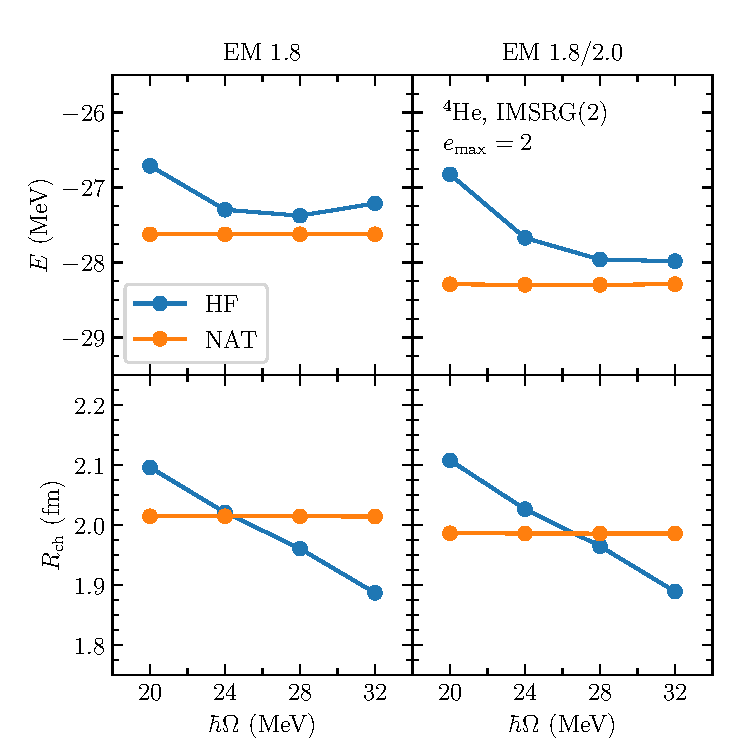
\includegraphics{thesis/doc/images/he4_imsrg2_results}
    \end{center}
    \caption{
        IMSRG(2) ground-state energies (top row) and charge radii (bottom row)
        of ${}^{4}\text{He}$
        for the NN-only EM 1.8 potential (left column)
        and the NN+3N EM 1.8/2.0 potential (right column)
        as a function of the oscillator frequency $\hbar \Omega$
        for the HF and NAT bases.
        The HF basis is constructed in $\emax=2$,
        and the NAT basis is constructed in $\emax=14$,
        with $E_{3\text{max}}=16$ for the NN+3N case,
        before being truncated to $\emax=2$ for the IMSRG(2) calculation.
    }\label{fig:he4_imsrg2_hf_nat}
\end{figure}

In this section,
we take a careful look at what happens to calculations for ${}^{4}\text{He}$
when we apply the IMSRG(3)-$N^7$ truncation.
For reference, we show in Fig.~\ref{fig:he4_imsrg2_hf_nat}
the results for the ground-state energy and charge radius
obtained via the IMSRG(2) for HF and NAT reference states
at various oscillator frequencies.
For the charge radius,
we use the
the square root
of the point-proton mean-square radius operator expectation value
and a spin-orbit correction~\cite{Ong10radius_spin_orbit}
added in quadrature.
We observe that the NAT basis
gives essentially frequency-independent results
for energies and radii
in both the NN-only and NN+3N cases.
The relatively strong frequency dependence
of the HF results is a consequence
of the construction of the HF basis in $\emax=2$.
The correlation energy
\begin{equation}
    E_{\text{corr}}\equiv E(s \rightarrow \infty) - E(s=0)\,,
\end{equation}
which is the contribution to the ground-state energy generated
by the many-body expansion,
is around 4 MeV for the NN-only calculations
and around 5 MeV for the NN+3N calculations.
When we compare the IMSRG(2) and IMSRG(3)-$N^7$ results,
it is sometimes illustrative to consider
their differences relative to $E_{\text{corr}}$,
since $E(s=0)$ is the same in both truncations
and they only differ in their many-body expansion order.
As a concrete example,
for the HF NN+3N case at $\hbar \Omega = 28\mev$,
$E(s=0) = -22.8145\mev$.
For the IMSRG(2) calculation,
$E(s \rightarrow \infty) = -27.9606\mev$
giving a correlation energy of
$E_{\text{corr}} = -5.1461\mev$.

\begin{figure}[t!]
    \begin{center}
        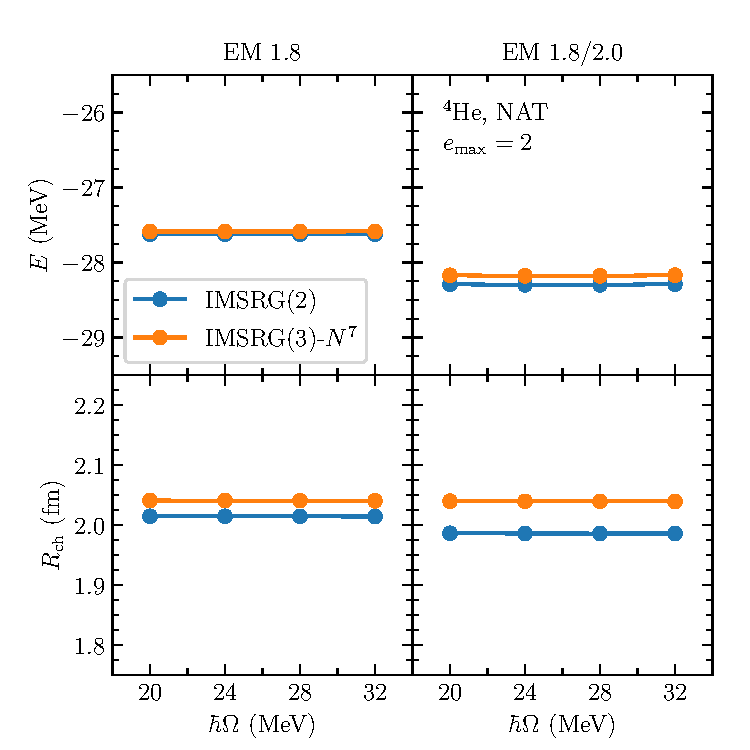
\includegraphics{thesis/doc/images/he4_NAT_results}
    \end{center}
    \caption{
        Ground-state energies (top row) and charge radii (bottom row)
        of ${}^{4}\text{He}$
        for the NN-only EM 1.8 potential (left column)
        and the NN+3N EM 1.8/2.0 potential (right column)
        as a function of the oscillator frequency $\hbar \Omega$
        for the NAT basis
        obtained via IMSRG(2) and IMSRG(3)-$N^7$ calulations.
        The NAT basis is constructed in $\emax=14$,
        with $E_{3\text{max}}=16$ for the NN+3N case,
        before being truncated to $\emax=2$ for the IMSRG calculations.
    }\label{fig:he4_imsrg3_nat}
\end{figure}

\begin{figure}[t!]
    \begin{center}
        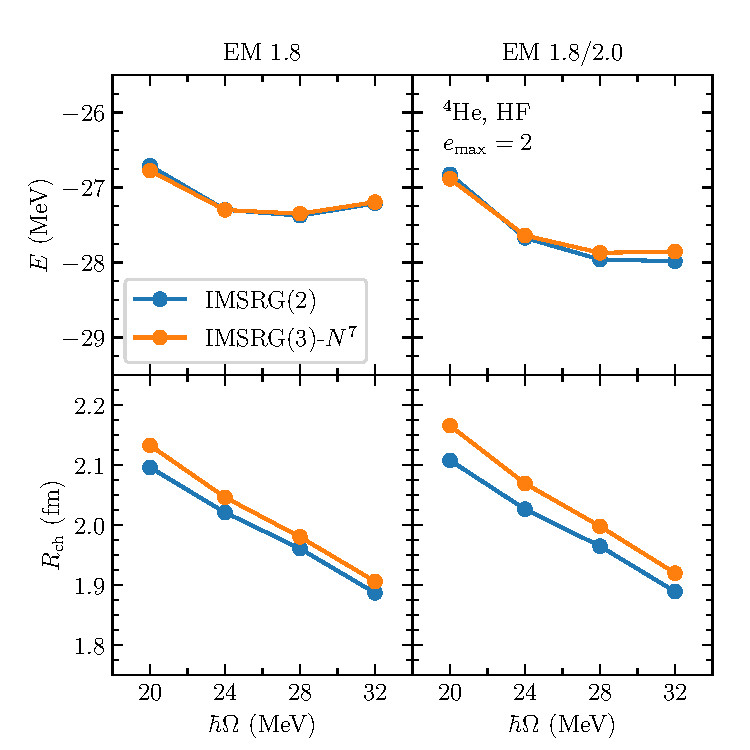
\includegraphics{thesis/doc/images/he4_HF_results}
    \end{center}
    \caption{
        Ground-state energies (top row) and charge radii (bottom row)
        of ${}^{4}\text{He}$
        for the NN-only EM 1.8 potential (left column)
        and the NN+3N EM 1.8/2.0 potential (right column)
        as a function of the oscillator frequency $\hbar \Omega$
        for the HF basis
        obtained via IMSRG(2) and IMSRG(3)-$N^7$ calulations.
        The HF basis is constructed in $\emax=2$.
    }\label{fig:he4_imsrg3_hf}
\end{figure}

The inclusion of 3N forces at the NO2B level gives
(in this system and for this model space)
a slightly larger binding energy
and accordingly a slightly smaller radius.
We emphasize that just the results from $\emax=2$
are not sufficient to make a statement
about the effect of 3N forces in ${}^{4}\text{He}$.
This is because in this model space
the Hamiltonian is not fully converged
with respect to model-space size
and so parts of the Hamiltonian could be cut out by the truncation
that would change the effect of 3N forces.
Thus, to make a concrete claim,
one must also do calculations for larger model spaces (currently out of reach)
and observe that the converged energies
change little as a function of $\emax=2$ to draw conclusions
about the contributions of 3N forces.

Incidentally,
in Jacobi-NCSM calculations, shown in Table~\ref{tab:ncsm_he4_results},
one sees that 3N forces do in fact
give a little bit more binding in ${}^{4}\text{He}$~\cite{Hebe20jac_nscm_he4}.
These values should not be compared with those from our IMSRG calculations
as the extrapolated values are converged with respect to model-space size
while our $\emax=2$ IMSRG results are not,
the $N_{\text{max}}$ truncation used in NCSM calculations
is different from the $\emax$ truncation used in many-body expansion methods,
and the calculation is based additonally on a Jacobi HO basis
instead of a single-particle basis like the single-particle NCSM and the IMSRG.
Additionally,
we use the NO2B approximation here,
which was seen to perform relatively poorly in ${}^{4}\text{He}$
in NCSM calculations~\cite{Roth11nonb_approx}
and is not present in the Jacobi-NCSM calulations discussed above.

In Fig.~\ref{fig:he4_imsrg3_nat},
we compare the results for
the ground-state energy and charge radius of ${}^{4}\text{He}$
for IMSRG(2) and IMSRG(3)-$N^7$ calculations
based on NAT reference states.
The frequency independence of the IMSRG(2) results
is preserved in the IMSRG(3)-$N^7$ results.
The three-body contributions to the ground-state energy
in the IMSRG(3)-$N^7$ are small,
37 keV in the NN-only case
and 120 keV in the NN+3N case.
The effect on the charge radius is more pronounced,
with a shift of 0.026 fm in the NN-only case
and 0.054 fm in the NN+3N case.

In Fig.~\ref{fig:he4_imsrg3_hf},
we see that the same trends are generally seen
for calculations based on HF reference states.
We see that the IMSRG(3)-$N^7$ results
for the energy are slightly flatter
as a function of oscillator frequency
than the IMSRG(2) results.
This may be a sign that the inclusion of three-body operators
in the IMSRG(3)-$N^7$ makes the IMSRG evolution
less sensitive to reference-state deficiencies.
However, to be able to conclude this,
this trend must be seen also for larger model spaces,
for other bases,
and for other closed-shell systems.


\section{Approximate IMSRG(3) truncation-scheme analysis}

\begin{figure}[t!]
    \begin{center}
        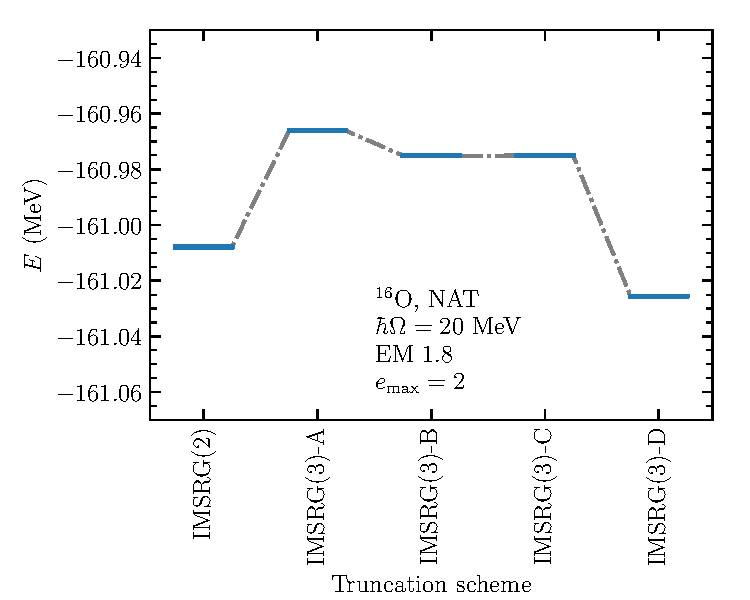
\includegraphics{thesis/doc/images/term_by_term_o16_plot}
    \end{center}
    \caption{
        Ground-state energies
        of ${}^{16}\text{O}$
        for the NN-only EM 1.8 potential
        resulting from IMSRG calculations
        using the IMSRG(2)
        and various approximated IMSRG(3) truncation schemes (see text for details).
        Calculations were done at an oscillator frequency of 20 MeV,
        and a NAT reference state was used.
        The NAT basis is constructed in $\emax=14$
        before being truncated to $\emax=2$ for the various many-body calculations.
    }\label{fig:term_by_term_o16}
\end{figure}

Now we turn our attention to what happens
when we turn on selected fundamental commutators
from the IMSRG(3) relative to the IMSRG(2) starting point.
For the purposes of this first exploration,
we consider ${}^{16}\text{O}$ in an $\emax=2$ model space.
We use the optimized NAT basis,
which delivers essentially frequency-independent results
for IMSRG(2) calculations of ${}^{16}\text{O}$.

In Fig.~\ref{fig:term_by_term_o16},
we show the ground-state energy of
${}^{16}\text{O}$
for various different truncation schemes
(see Sec.~\ref{sec:imsrg3_truncation_schemes} for details).
For all of these calculations, $E_{\text{corr}} \sim 10$ MeV.
We see that the first stable IMSRG(3) approximation,
the IMSRG(3)-A truncation,
produces a sizable shift in the energy of 42 keV.
This is to be contrasted with the next two truncations,
IMSRG(3)-B,
which adds all $\mathcal{O}(N^6)$ IMSRG(3) fundamental commutators
to IMSRG(3)-A,
and IMSRG(3)-C (or IMSRG(3)-$N^7$),
which adds the final remaining $\mathcal{O}(N^7)$ IMSRG(3) fundamental commutator
to IMSRG(3)-B,
where the energy shifts by 9 keV and 0.2 keV respectively.
In this sense,
it seems as though the IMSRG(3)-$N^7$ truncation
is dominated by the commutators included in the IMSRG(3)-A truncation
and the commutators included in the IMSRG(3)-B and IMSRG(3)-C truncations
do relatively little.
We note that for the three commutators added in the IMSRG(3)-B truncation
each commutator separately has a small contribution,
and it is not the case that two commutators have relatively large contributions
that cancel to give an overall small contribution.

The organization outlined in Section~\ref{sec:imsrg3_truncation_schemes}
is primarily based on computational cost.
In light of this organization,
it is interesting that the contribution from the first
$\mathcal{O}(N^8)$ commutator included in the IMSRG(3)-D truncation scheme
is quite large,
producing a 51 keV shift in the ground-state energy.
This suggests that the organization by cost may not be not well motivated
and in practice does not behave desirably when
going from IMSRG(2) to IMSRG(3).
To develop better approximated IMSRG(3) truncation schemes,
one could perform a perturbative analysis as is done in Chapter 7 of Ref.~\cite{Herg15imsrgphysrep}
for IMSRG(2),
where it is shown that IMSRG(2) is exact up to third order in MBPT.
Doing this for IMSRG(3)
would allow one to determine which commutators
to include to make an approximate IMSRG(3) truncation complete
up to some order in MBPT.


\chapter{Summary and outlook}\label{ch:summary}

The aim of this thesis was to investigate
the contributions of induced three-body operators
in the IMSRG.
To this end,
we studied the IMSRG(3) truncation
of the IMSRG.
The uncoupled ($m$-scheme) implementation of the IMSRG(3)
is too expensive for nuclear applications,
so we exploited the spherical symmetry
of the IMSRG
when applied to closed-shell nuclei
to arrive at the $J$-scheme IMSRG(3)
fundamental commutators.
We implemented an IMSRG(2)/(3) solver
using these fundamental commutators
that is more performant than
the previous $m$-scheme implementation.
With this implementation in hand,
we were able to do first explorations
of the effects of approximations to the IMSRG(3) truncation
when compared with the IMSRG(2) truncation in ${}^{4}\text{He}$
and ${}^{16}\text{O}$.

To allow for the exploration of different single-particle bases,
Hamiltonians, and oscillator frequencies,
we introduced several approximate IMSRG(3) truncation schemes
that leave out the most expensive fundamental commutators,
one of which was the IMSRG(3)-$N^7$.
We find that in ${}^{4}\text{He}$,
the IMSRG(3)-$N^7$ truncation
offers a small correction at the sub-percent level
to the IMSRG(2) result
for the ground-state energy
in the $\emax=2$ model space considered.
The corrections to the charge radius are larger,
on the order of a few percent.
We see that the IMSRG(3)-$N^7$
performs somewhat better than the IMSRG(2)
away from the optimal HF oscillator frequency,
a trend that needs to be verified
for larger model spaces and different systems.

For ${}^{16}\text{O}$,
we considered
various approximate IMSRG(3) truncation schemes.
These schemes were set up to include
one or several fundamental commutators
on top of the previous truncation scheme,
starting from the IMSRG(2).
The organization of these schemes was
partially physically motivated
(in particular the IMSRG(3)-A scheme),
but most commutator inclusions
were organized by computational cost.
We found that this organization
did not deliver the desired results.
While the IMSRG(3)-A truncation
provided a relatively significant shift
from the IMSRG(2) results,
the inclusion of the remaining
$\mathcal{O}(N^6)$ and
$\mathcal{O}(N^7)$ commutators
provided only small corrections
to the ground-state energy of ${}^{16}\text{O}$.
The final truncation scheme we considered,
which included the first $\mathcal{O}(N^8)$
commutator,
produced another large shift over the previous truncation.
This suggests that computational cost
is not a good proxy for importance in the formation of
an approximate IMSRG(3) truncation.

Looking to the future,
there are clear objectives for our IMSRG(3) implementation.
The first is tuning the performance of the implementation
to put full IMSRG(3) $\emax=6$ and hopefully $\emax=8$
within reach.
Additional restrictions can be placed on
for example the range of three-body channels,
potentially allowing IMSRG(3) calculations
to reach even larger single-particle model space sizes.
This will allow us to perform converged IMSRG(3) calculations
for medium-mass nuclei
and investigate what effects it has on observables.
Parallel to this,
obtaining exact (full configuration interaction) results
in $\emax=2$
would allow us to see how IMSRG(3)
compares with IMSRG(2)
relative to the exact solution
of the Schr{\"o}dinger equation
in $\emax=2$.
A secondary implementation goal
is the support of tensor operators,
which would give our implementation access to many more observables,
such as low-lying spectroscopy.

A key result of this thesis is that the organization by computational cost,
at least for the limited calcuations discussed here
for which we lack exact results
provided by full configuration interaction calculations,
is not a good strategy for developing an IMSRG(3) approximation.
To develop the IMSRG(3) further,
a more careful look into the behavior and structure of the fundamental commutators
is important
to understand the deficiencies in the naive organization by cost.
One path to doing this is the perturbative analysis
of the IMSRG(3) flow equations.
This could allow one to develop an approximate IMSRG(3) truncation
that is potentially fourth- or fifth-order exact in MBPT.
This analysis will need to be adapted
to account for non-HF reference states
and also cases beyond the NO2B approximation
where the residual normal-ordered three-body Hamiltonian
is included at the start of the IMSRG calculation.
In this analysis of the IMSRG(3),
it will be interesting to look at how the IMSRG(3)
performs relative to the IMSRG(2) under variation of the reference state.
If one finds that the IMSRG(3) is more successful
for sub-optimal reference states,
understanding this feature of the IMSRG(3)
may allow for constructions of IMSRG(3) approximations
that share this behavior.

This thesis represents a first step
towards full IMSRG(3) calculations
of light and medium-mass nuclei
and the systematic development and testing
of approximate IMSRG(3) truncation schemes.
Accessing full IMSRG(3) calculations
will provide access to high-precision many-body results,
hopefully bringing the many-body uncertainty error
for ground-state energies robustly into the per-mille range.
Well-motivated approximations of the IMSRG(3)
will make most of the accuracy benefits of the IMSRG(3)
available at a lower computational cost,
necessary for calculations where large model spaces
are required to converge calculations,
for example for heavy nuclei or hard, unevolved nuclear Hamiltonians.


\begin{appendices}

  \chapter{\texorpdfstring{$m$-scheme}{M-scheme} fundamental commutators for the IMSRG(3)}\label{app:mscheme_fundamental_commutators}

We list the $m$-scheme fundamental commutators needed for the IMSRG(3),
taken from Ref.~\cite{Herg15imsrgphysrep}.
The commutator of a $K$-body and an $L$-body operator
gives $|K-L|$- to $(K+L-1)$-body terms:
\begin{equation}
  \left[A^{(K)}, B^{(L)}\right] = \sum_{M=|K - L|}^{K + L - 1} C^{(M)}\,.
\end{equation}
Note that the expressions we give below are
for the matrix elements of the different $M$-body terms.
Also note that expressions for two- and three-body matrix elements
are not antisymmetrized,
so the appropriate antisymmetrizer must be applied
to the matrix elements after evaluating the commutator.
We use the convention that the index labels $i$,~$j$,~$k$,~\ldots\
are reserved for external indices,
that is, indices appearing on the matrix elements of the resulting operator,
and the index labels $a$,~$b$,~$c$,~\ldots\
are reserved for contracted indices,
that is, indices that are summed over in the matrix elements of the input operators.
$n_a$ are the occupation numbers,
and $\bar{n}_a = 1 - n_a$.

\section{
  \texorpdfstring{$[\onebodyop{A}, \onebodyop{B}]$}{[1, 1]}
 }

The commutator of two one-body operators
has a zero-body part,
\begin{equation}
  C = \sum_{ab} (n_a - n_b) A_{ab} B_{ba}\,,
\end{equation}
and a one-body part
\begin{equation}
  C_{ij} = \sum_{a}(A_{ia} B_{aj} - B_{ia} A_{aj})\,.
\end{equation}

\section{
  \texorpdfstring{$[\onebodyop{A}, \twobodyop{B}]$}{[1, 2]}
 }

The commutator of a one-body operator and a two-body operator
has a one-body part,
\begin{equation}
  C_{ij} = \sum_{ab} (n_a - n_b) A_{ab} B_{biaj}\,,
\end{equation}
and a two-body part,
\begin{equation}
  C_{ijkl} = 2 \sum_{a} (A_{ia} B_{ajkl} - A_{ak} B_{ijal})\,.
\end{equation}

\section{
  \texorpdfstring{$[\twobodyop{A}, \twobodyop{B}]$}{[2, 2]}
 }

The commutator of two two-body operators
has a zero-body part,
\begin{equation}
  C = \frac{1}{4} \sum_{abcd}
  (n_a n_b \bar{n}_c \bar{n}_d - \bar{n}_a \bar{n}_b n_c n_d)
  A_{abcd} B_{cdab}\,,
\end{equation}
a one-body part,
\begin{equation}
  C_{ij} = \frac{1}{2} \sum_{abc}
  (\bar{n}_a \bar{n}_b n_c + n_a n_b \bar{n}_c)
  (A_{ciab} B_{abcj} - B_{ciab} A_{abcj})\,,
\end{equation}
a two-body part,
\begin{equation}
  C_{ijkl} = D_{ijkl} + E_{ijkl}\,,
\end{equation}
with
\begin{align}
  D_{ijkl} & \equiv \frac{1}{2} \sum_{ab} (\bar{n}_a - n_b)
  (A_{ijab} B_{abkl} - B_{ijab} A_{abkl})\,,                     \\
  E_{ijkl} & \equiv 4 \sum_{ab} (n_a - n_b) A_{aibk} B_{bjal}\,,
\end{align}
and a three-body part,
\begin{equation}
  C_{ijklmn} = 9 \sum_{a} (A_{ijla} B_{akmn} - B_{ijla} A_{akmn})\,.
\end{equation}

\section{
  \texorpdfstring{$[\onebodyop{A}, \threebodyop{B}]$}{[1, 3]}
 }

The commutator of a one-body operator and a three-body operator
has a two-body part,
\begin{equation}
  C_{ijkl} = \sum_{ab} (n_a - n_b) A_{ab} B_{bijakl}\,,
\end{equation}
and a three-body part,
\begin{equation}
  C_{ijklmn} = 3 \sum_{a} (
  A_{ia} B_{ajklmn} - A_{al} B_{ijkamn}
  )\,.
\end{equation}

\section{
  \texorpdfstring{$[\twobodyop{A}, \threebodyop{B}]$}{[2, 3]}
 }

The commutator of a two-body operator and a three-body operator
has a one-body part,
\begin{equation}
  C_{ij} = -\frac{1}{4} \sum_{abcd}
  (n_a n_b \bar{n}_c \bar{n}_d - \bar{n}_a \bar{n}_b n_c n_d)
  A_{cdab} B_{abijcd}\,,
\end{equation}
a two-body part,
\begin{equation}
  C_{ijkl} = - \sum_{ab}
  (n_a \bar{n}_b \bar{n}_c + \bar{n}_a n_b n_c)
  (A_{bcak} B_{aijbcl} + A_{bcai} B_{aklbcj})\,,
\end{equation}
and a three-body part,
\begin{equation}
  C_{ijklmn} = \frac{3}{2} \sum_{ab} (\bar{n}_a - n_b)
  (A_{ijab} B_{abklmn} - A_{abmn} B_{ijklab})\,.
\end{equation}

\section{
  \texorpdfstring{$[\threebodyop{A}, \threebodyop{B}]$}{[3, 3]}
 }

The commutator of two three-body operators
has a zero-body part,
\begin{equation}
  C = \frac{1}{36} \sum_{abcdef}
  (
  n_a n_b n_c \bar{n}_d \bar{n}_e \bar{n}_f
  - \bar{n}_a \bar{n}_b \bar{n}_c n_d n_e n_f
  )
  A_{abcdef} B_{defabc}\,,
\end{equation}
a one-body part,
\begin{equation}
  C_{ij} = \frac{1}{12}
  \sum_{abcde} (
  n_a n_b \bar{n}_c \bar{n}_d \bar{n}_e
  + \bar{n}_a \bar{n}_b n_c n_d n_e
  )
  (
  A_{abicde} B_{cdeabj}
  - B_{abicde} A_{cdeabj}
  )\,,
\end{equation}
a two-body part,
\begin{equation}
  C_{ijkl} = D_{ijkl} + E_{ijkl}\,,
\end{equation}
with
\begin{align}
  D_{ijkl} & \equiv \frac{1}{6} \sum_{abcd}
  (
  n_a \bar{n}_b \bar{n}_c \bar{n}_d
  - \bar{n}_a n_b n_c n_d
  )
  (
  A_{aijbcd} B_{bcdakl}
  - B_{aijbcd} A_{bcdakl}
  )\,,                                      \\
  E_{ijkl} & \equiv \sum_{abcd}
  (
  \bar{n}_a \bar{n}_b n_c n_d
  - n_a n_b \bar{n}_c \bar{n}_d
  )
  A_{abicdl} B_{cdjabk}\,,
\end{align}
and a three-body part,
\begin{equation}
  C_{ijklmn} = D_{ijklmn} + E_{ijklmn} + F_{ijklmn}\,,
\end{equation}
with
\begin{align}
  D_{ijklmn} & \equiv \frac{1}{6} \sum_{abc}
  (n_a n_b n_c + \bar{n}_a \bar{n}_b \bar{n}_c)
  (A_{ijkabc} B_{abclmn} - B_{ijkabc} A_{abclmn})\,, \\
  E_{ijklmn} & \equiv \frac{9}{2} \sum_{abc}
  (n_a n_b \bar{n}_c +  \bar{n}_a \bar{n}_b n_c)
  A_{abkcmn} B_{cijabl}\,,                           \\
  F_{ijklmn} & \equiv -\frac{9}{2} \sum_{abc}
  (n_a n_b \bar{n}_c +  \bar{n}_a \bar{n}_b n_c)
  A_{cjkabn} B_{iablmc}\,.
\end{align}

  \chapter{Simplification strategies for coupled fundamental commutators}\label{app:jscheme_commutator_tricks}

For the coupled fundamental commutators,
the key to arriving at the simplest expressions
is to avoid unnecessary recoupling.
Recoupling,
where bra or ket couplings have to be broken and recreated
to relate matrix elements on both sides of the expression,
is unnecessary when symmetries of the matrix elements
or of the expression can be exploited
to bring the uncoupled expression into a form
where its coupled analog no longer requires recoupling.
Recoupling comes at the cost of an additional sum over an angular momentum
and the inclusion of a Wigner $6j$ or $9j$ symbol.
Thus avoiding unnecessary recoupling is essential for achieving better performance
for implementations of the coupled expressions.
In the following,
we discuss two strategies for avoiding recoupling
and apply them each to one example.

\section{Using antisymmetry of input operator matrix elements}

The uncoupled matrix elements are antisymmetric under exchange
of any two bra or ket indices.
This symmetry can easily be exploited to permute indices into a form
that minimizes recoupling.

Consider the $[\onebodyop{A}, \threebodyop{B}] \rightarrow \twobodyop{C}$ fundamental commutator.
The uncoupled expression for the matrix elements of $C$ is
\begin{equation}
    C_{ijkl} = \sum_{ab} (n_a - n_b) A_{ab} B_{bijakl}\,,
\end{equation}
and the coupled expression is
\begin{equation}
    \begin{split}
        C_{ijkl}^{J_C} &= (-1)^{j_i + j_j + j_k + j_l}
        \sum_{j_a} \sum_{(J_{B,3}, J_{B,pq}, J_{B,st})} \hat{J}_{B,pq}\hat{J}_{B,st}\hat{J}_{B,3}^2 \\
        &\quad\sum_{ab} (n_a \bar{n}_b - \bar{n}_a n_b)
        \sixj{j_j}{j_i}{J_C}{j_a}{J_{B,3}}{J_{B,pq}}
        \sixj{j_l}{j_k}{J_C}{j_a}{J_{B,3}}{J_{B,st}} \\
        &\quad A_{ab}^{j_a} B_{bijakl}^{(J_{B,3}, J_{B,pq}, J_{B,st})}\,.
    \end{split}
\end{equation}

The appearance of 6$j$ symbols is a result of
breaking the $bi$ coupling on the right to form the $ij$ coupling on the left
and breaking the $ak$ coupling on the right to form the $kl$ coupling on the left.
By exploiting antisymmetry in the uncoupled matrix elements of $B$,
we can arrive at the uncoupled expression
\begin{equation}
    C_{ijkl} = \sum_{ab} (n_a \bar{n}_b - \bar{n}_a n_b) A_{ab} B_{ijbkla}\,,
\end{equation}
which yields the coupled expression
\begin{equation}
    C_{ijkl}^{J_C} = \frac{1}{\hat{J}_{C}^2}
    \sum_{j_a}
    \sum_{J_{B,3}} \hat{J}_{B,3}^2
    \sum_{ab} (n_a \bar{n}_b - \bar{n}_a n_b)
    A_{ab}^{j_a} B_{ijbkla}^{(J_{B,3}, J_{C}, J_{C})}\,.
\end{equation}

\section{Using antisymmetry of output operator matrix elements}

As a reminder, in this work we typically work with
non-antisymmetrized expressions for the fundamental commutators,
so one can not simply permute the indices on the output matrix elements.
However, one can exploit that the output matrix elements
will at some point be antisymmetrized
and choose the term that contributes to the antisymmetrized result
with the minimal recoupling.

To make this clear, consider the following example:
Suppose the three-body uncoupled matrix elements $O_{pqrstu}$
are already antisymmetric in $stu$, but not in $pqr$.
Thus to get the final antisymmetrized matrix elements $O^{\text{as}}_{pqrstu}$,
one needs to evaluate
\begin{equation}\label{eq:antisymmetrize_short}
    O^{\text{as}}_{pqrstu} = \mathcal{A}_{pqr} O_{pqrstu}\,,
\end{equation}
with
\begin{equation}
    \mathcal{A}_{pqr} = \frac{1}{6} (1 + P_{prq} + P_{prq}^2) (1 - P_{pq})\,,
\end{equation}
where $P_{prq}$ cyclically permutes the indices $p$, $q$, and $r$
and $P_{pq}$ exchanges the indices $p$ and $q$
as discussed in Section~\ref{sec:jscheme_many_body_expressions}.

Writing Eq.~\eqref{eq:antisymmetrize_short} out, one gets
\begin{equation}\label{eq:antisymmetrize_long_normal}
    O^{\text{as}}_{pqrstu} = \frac{1}{6} (O_{pqrstu} + O_{qrpstu} + O_{rpqstu} - O_{qprstu} - O_{rqpstu} - O_{prqstu})\,.
\end{equation}
Now consider
\begin{equation}
    \overline{O}_{pqrstu} \equiv O_{qrpstu}\,.
\end{equation}
Antisymmetrizing $\overline{O}_{pqrstu}$ gives
\begin{equation}
    \overline{O}^{\text{as}}_{pqrstu} = \frac{1}{6} (\overline{O}_{pqrstu} + \overline{O}_{qrpstu} + \overline{O}_{rpqstu}
    - \overline{O}_{qprstu} - \overline{O}_{rqpstu} - \overline{O}_{prqstu})\,,
\end{equation}
which one can rewrite in terms of the original matrix elements $O_{pqrstu}$:
\begin{equation}\label{eq:antisymmetrize_long_alternate}
    \overline{O}^{\text{as}}_{pqrstu} = \frac{1}{6} (O_{qrpstu} + O_{rpqstu} + O_{pqrstu}
    - O_{rqpstu} - O_{prqstu} - O_{qprstu})\,.
\end{equation}
One can quickly see that Eqs.~\eqref{eq:antisymmetrize_long_normal} and~\eqref{eq:antisymmetrize_long_alternate}
contain the exact same terms, making them equal.
Thus if $O_{pqrstu}$ is given by some many-body expression,
one can permute the indices $p$, $q$, and $r$ on the right-hand (or left-hand) side of the expression,
including an overall minus sign if the permutation is odd,
and know that it will give the same result after antisymmetrization.

Again, it is useful to consider a concrete application to illustrate how this strategy can be applied.
Consider the $[\twobodyop{A}, \twobodyop{B}] \rightarrow \threebodyop{C}$ fundamental commutator.
The uncoupled non-antisymmetrized expression is
\begin{equation}
    C_{ijklmn} = 9 \sum_{a} (A_{ijla} B_{akmn} - B_{ijla} A_{akmn})\,.
\end{equation}
which gives the coupled expression
\begin{equation}\label{eq:comm_223_bad}
    \begin{split}
        C_{ijklmn}^{(J_{C,3}, J_{C,ij}, J_{C,lm})} & =
        9 \hat{J}_{C,ij} \hat{J}_{C,lm}
        (-1)^{j_m + j_n}
        \sum_{J_{mn}}
        \hat{J}_{mn}^2
        \sum_{a} (-1)^{j_a + j_k} \\
        & \quad \quad \times
        \sixj{j_k}{j_a}{J_{mn}}{j_{l}}{J_{C,3}}{J_{C,ij}}
        \sixj{j_l}{j_m}{J_{C,lm}}{j_{n}}{J_{C,3}}{J_{mn}} \\
        & \quad \quad \times \left(
        A_{ijla}^{J_{C,ij}} B_{akmn}^{J_{mn}}
        - B_{ijla}^{J_{C,ij}} A_{akmn}^{J_{mn}}
        \right).
    \end{split}
\end{equation}
One can immediately see that
the $mn$ coupling on the right in $B$ and $A$ needs to be broken up
to form the $lm$ coupling on the left,
leading to some of the recoupling.

However, the uncoupled expression
\begin{equation}
    D_{ijklmn} \equiv 9 \sum_{a} (A_{ijna} B_{aklm} - B_{ijna} A_{aklm})
\end{equation}
has the indices $l$, $m$, and $n$ on the right-hand side permuted cyclically,
and it will no longer have this recoupling problem when the expression is coupled.
The antisymmetrized matrix elements of $C$ and $D$ are equal,
so one might as well simply calculate $D$ instead of $C$ and antisymmetrize that.
The coupled expression for $D$ is
\begin{equation}\label{eq:comm_223_good}
    \begin{split}
        D_{ijklmn}^{(J_{C,3}, J_{C,ij}, J_{C,lm})} & =
        -9 (-1)^{J_{C,lm}} \hat{J}_{C,ij} \hat{J}_{C,lm}
        \sum_{a} (-1)^{j_a + j_k}
        \sixj{j_k}{j_a}{J_{C,lm}}{j_{n}}{J_{C,3}}{J_{C,ij}} \\
        & \quad \quad \times \left(
        A_{ijna}^{J_{C,ij}} B_{aklm}^{J_{C,lm}}
        - B_{ijna}^{J_{C,ij}} A_{aklm}^{J_{C,lm}}
        \right).
    \end{split}
\end{equation}
The final $6j$ symbol cannot be avoided
as it forms the three-body angular-momentum coupling
that is not present on the right-hand side.
Comparing Eq.~\eqref{eq:comm_223_bad} and Eq.~\eqref{eq:comm_223_good},
one can see the simplification afforded by carefully considering
which quantity one actually wants to calculate.

  \chapter{IMSRG(3) for the pairing Hamiltonian}\label{app:pairing_hamiltonian_imsrg3}

The pairing Hamiltonian is given by
\begin{equation}\label{eq:pairing_hamiltonian}
    H = \delta \sum_{p\sigma} (p - 1) \crea{p\sigma} \annih{p\sigma}
    - \frac{g}{2} \sum_{p q} \crea{p+}\crea{p-} \annih{q-} \annih{q+}\,,
\end{equation}
where we have equally-spaced two-fold degenerate levels indexed by the quantum number $p$
and an attractive (for $g > 0$) pairing interaction.
Cooper first considered this Hamiltonian in 1956~\cite{Coop56pairing_hamiltonian},
which led to the successful Bardeen-Cooper-Schreifer (BCS) theory of superconductivity~\cite{Bard57bcs}.
The exact eigenvalues of the pairing Hamiltonian were given by Richardson in 1963,
where the solutions are obtained via the solution of the non-linear coupled Richardson equations~\cite{Rich63pairing_hamiltonian}.

We focus on a restricted case where $p=1,\ldots,4$ and $\delta=1\mev$,
and we vary the strength of the pairing interaction $g$.
We are interested in the ground state of four fermions,
for which our reference state is the state with the two lowest levels completely filled,
\begin{equation}\label{eq:pairing_hamiltonian_reference}
    \refgnd = \crea{2-}\crea{2+}\crea{1-}\crea{1+}\ket{0}\,.
\end{equation}
This system has a couple of useful properties:
First, the number of single-particle states is only eight,
making the IMSRG(3) calculation relatively tractable.
Additionally, one can increase the number of levels $p_{\text{max}}$ easily
to get a handle on the performance for larger single-particle basis sizes.
Second, in addition to the available exact solution,
this system is easy to construct and diagonalize in the basis
of the reference state and its particle-hole excitations,
\begin{equation}
    \{\refgnd, \refhp{ij}{ab}, \refhp{ijkl}{abcd} \}\,,
\end{equation}
where the odd number particle-hole excitations do not contribute
as Eq.~\eqref{eq:pairing_hamiltonian} only couples pairs.
This makes it easy to obtain an exact solution with which to compare the IMSRG(2)
and IMSRG(3) solutions.
Finally, after normal ordering the Hamiltonian with respect to our reference state,
we find that $\hnoone$ is diagonal,
meaning our reference state is the canonical Hartree-Fock reference state
with the Hartree-Fock energy $\hnozero=E_{\text{HF}}=2 - g$.
This means the IMSRG evolution must only bring in correlation corrections to the energy
without needing to overcome any reference state deficiencies.

\begin{figure}[t]
    \centering
    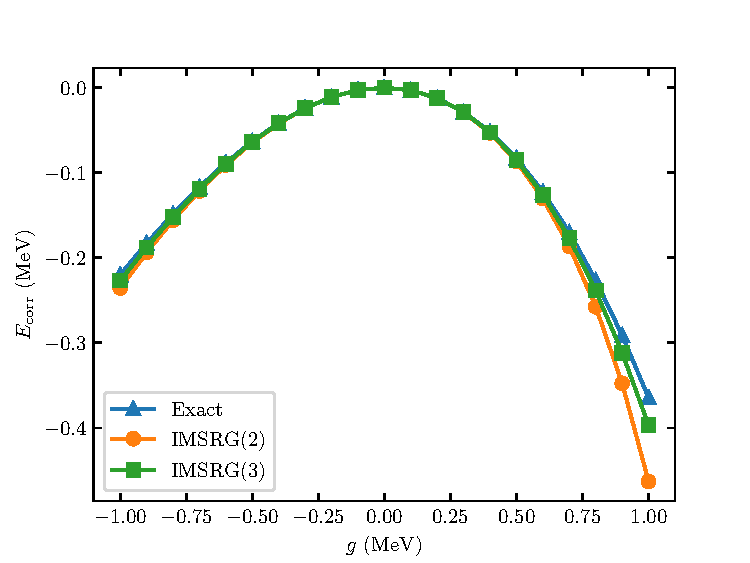
\includegraphics[width=0.9\textwidth]{thesis/doc/images/pairing_ham_imsrg3.pdf}
    \caption[
        The correlation energy $E_{\text{corr}}$ for the solution of the pairing Hamiltonian
        obtained via exact diagonalization,
        IMSRG(2), and IMSRG(3)
        for $-1 \le g \le 1$.
    ]{
        The correlation energy $E_{\text{corr}}$ for the solution of the pairing Hamiltonian
        obtained via exact diagonalization,
        IMSRG(2), and IMSRG(3)
        for $-1 \le g \le 1$.
        Exact diagonalization results obtained using code published with Ref.~\cite{Liet16lecnotesphysics}.
    }\label{fig:pairing_hamiltonian_fig}
\end{figure}

Thus, we are interested in the correlation energy obtained by the IMSRG(2) and IMSRG(3) solutions,
defined as
\begin{equation}
    E_{\text{corr}} \equiv E(s \rightarrow \infty) - E(s= 0)\,.
\end{equation}
This is plotted in Fig.~\ref{fig:pairing_hamiltonian_fig} for $-1 \le g \le 1$.
We find generally good agreement between the IMSRG correlation energy
and the exact correlation energy,
with the exception of the region for $0.5 \le g \le 1$.
Here, the IMSRG(3) calculation improves upon the relatively large error in the IMSRG(2)
correlation energy,
which in Ref.~\cite{Herg16imsrglecnotes}
was explained as being due to an overcounting in the fourth-order diagrams in MBPT
by a factor of 1/2 present in the IMSRG(2) truncation.
It seems that this overcounting at fourth-order is lifted in the IMSRG(3).
We note here that our results for IMSRG(2) match exactly with those from Ref.~\cite{Herg16imsrglecnotes}.


\end{appendices}

\backmatter{}

\bibliographystyle{apsrev4-1-mh-mod} % use your favorite BIBTeX style
% \nocite{*} % To display all refs, even uncited refs (useful when editting)
\bibliography{sources}

\end{document}

